\documentclass[a4paper,twoside,openright,12pt]{report}

\usepackage[T1]{fontenc}
\usepackage[utf8]{inputenc}
\usepackage{lmodern}
\usepackage{layout}
\usepackage{emptypage}
\usepackage{fancyhdr}
\usepackage[activeacute,spanish]{babel}
\usepackage{graphicx}
\usepackage{caption}
\usepackage{subcaption}
\usepackage{mathtools}
\usepackage[Lenny]{fncychap}
\usepackage{hyperref}
\usepackage[a4paper,top=3.5cm, bottom=3cm, inner=3cm, outer=2.5cm]{geometry}
\usepackage{listings}
\usepackage{enumerate}
\usepackage{cite}

%For inserting pretty code
\usepackage{color}
\definecolor{gray97}{gray}{.97}
\definecolor{gray75}{gray}{.75}
\definecolor{gray45}{gray}{.45}

\usepackage{listings}
\lstset{ frame=Ltb,
framerule=0pt,
aboveskip=0.5cm,
framextopmargin=3pt,
framexbottommargin=3pt,
framexleftmargin=0.4cm,
framesep=0pt,
rulesep=.4pt,
backgroundcolor=\color{gray97},
rulesepcolor=\color{black},
%
stringstyle=\ttfamily,
showstringspaces = false,
basicstyle=\small\ttfamily,
commentstyle=\color{gray45},
keywordstyle=\bfseries,
%
numbers=left,
numbersep=15pt,
numberstyle=\tiny,
numberfirstline = false,
breaklines=true,
}

% minimizar fragmentado de listados
\lstnewenvironment{listing}[1][]
{\lstset{#1}\pagebreak[0]}{\pagebreak[0]}

\lstdefinestyle{consola}
{basicstyle=\scriptsize\bf\ttfamily,
backgroundcolor=\color{gray75},
}
\lstdefinestyle{python}
{language=python,
}
\lstdefinestyle{C}
{language=C,
}

\headheight=16pt
\pretolerance=10000
\renewcommand{\lstlistingname}{Código}

\pagestyle{fancy}
\renewcommand{\chaptermark}[1]{\markboth{\chaptername	\ \thechapter.\ #1}{}}
\renewcommand{\sectionmark}[1]{\markright{\thesection.\ #1}}

\fancyhf{}
%\fancyhead[LO,RE]{\leftmark} % Nombre de capítulo
\fancyhead[LE,RO]{\rightmark} % Nombre de sección
\fancyfoot[C]{\thepage}

\pagestyle{empty}

\title{VisualHFSM 5.0}
\author{Samuel Rey Escudero}

\lstset{
	float=hbp,
	basicstyle=\ttfamily\small,
	columns=flexible,
	tabsize=4,
	frame=single,
	extendedchars=true,
	showspaces=false,
	showstringspaces=false,
	numbers=none,
	numberstyle=\tiny,
	breaklines=false,
	breakautoindent=true,
	captionpos=b
}

\begin{document}

%%%%%%%%%%%%%%% Portada %%%%%%%%%%%%%%%%%%%%
\hypersetup{pageanchor=false}
\begin{titlepage}
	\centering
	
\includegraphics[width=0.6\linewidth]{imgs/logoURJC}\par
	\vspace{2.5cm}
	{\scshape\LARGE Ingeniería en Tecnologías de la Telecomunicación\par}
	\vspace{2cm}
	{\scshape\Large Trabajo fin de grado\par}
	\vspace{1.5cm}
	{\huge\bfseries VisualHFSM 5.0\par}
	\vspace{2.5cm}
	\vfill
	\textbf{Autor:} Samuel Rey Escudero\par
	\textbf{Tutor:} Prof. José María Cañas\par
	\vspace{2.5cm}
	{\large Curso académico 2015/2016}
\end{titlepage}

\pagebreak
\thispagestyle{empty}
\vspace*{14cm}

\begin{flushright}
	
\includegraphics[height=1.0cm]{imgs/by-sa}\par
\vspace*{0.5cm}
\copyright 2016 Samuel Rey Escudero\par
\vspace*{0.3cm}
Esta obra está distribuida bajo la licencia de ``Reconocimiento-CompartirIgual 4.0 Internacional (CC BY-SA 4.0)'' de Creative Commons.\par
\vspace{0.2cm}
Para ver una copia de esta licencia, visite http://creativecommons.org/licenses/by-sa/4.0/ o envíe una carta a Creative Commons, 171 Second Street, Suite 300, San Francisco, California 94105, USA.
\end{flushright}

%\layout % Imprime un esquema con el layout.

\pagenumbering{Roman} % para comenzar la numeración de paginas en números romanos
\hypersetup{pageanchor=true}

%%%%%%%%%%%%%%% Agradecimientos %%%%%%%%%%%%
\clearpage
\chapter* {Agradecimientos}
En primer lugar, me alegro mucho de haber escogido este tema como trabajo de fin de grado. Gracias a él he descubierto el apasionante mundo de la robótica, y me ha servido tanto a nivel académico, pues al ser un tema que no se toca en mi grado, me ha servido para conseguir una formación más completa, como a nivel personal, pues ha despertado en mi un fuerte interés por este tema. \\

Quiero darles las gracias a Rubén y Borja, pues sus anteriores trabajos\cite{salamanques2012, borja2014} han supuesto una enorme cantidad de información para mi y me ha facilitado mucho la elaboración del trabajo, ayudándome especialmente a entender somo funcionaba mientras daba mis primeros pasos con VisualHFSM. \\

También quiero darle las gracias a Carlos Bazaga, pues ha aportado el código para seguir la carretera, con el que he estado atascado bastante tiempo. \\

Por supuesto, gracias a Jose María por su labor como tutor, cuya paciencia y consejos han ayudado a llevar este trabajo siempre un poco más allá. \\

Por último, quiero aprovechar esta ocasión para darle las gracias a mi familia y mis amigos, por estar siempre ahí cuando los he necesitado, ofreciéndome apoyo y distracciones. \\

Y por su puesto, muchas gracias a mi novia, Celia, que ha hecho posible que esté siempre positivo y seguro de mi mismo, apoyándome para seguir avanzando y ayudándome a olvidarme de todo cuando más lo he necesitado.
\clearpage
%%%%%%%%%%%%%%% Resumen %%%%%%%%%%%%%%%%%%%%
\chapter* {Resumen}

La robótica es un campo que está experimentando una expansión y desarrollo nunca antes visto, utilizándose cada vez en más aplicaciones y más variadas. Uno de los factores determinantes para esto radica en la inteligencia de los robots, su programación, por lo que muchos lenguajes han ido adaptándose a esta rama facilitando cada vez más su uso en la programación de robots. Además, han aparecido alternativas distintas a la programación tradicional, como los lenguajes de programación visual o el uso de máquinas de estados para representar fácilmente el comportamiento de los robots. \\

En estos dos pilares se apoya nuestra herramienta, VisualHFSM. esta herramienta se sitúa dentro de la plataforma JdeRobot y facilita la programación de comportamientos de robots generando gran parte del código. Para esto, el flujo de control se representa visualmente mediante un diagrama de estados, de forma que el desarrollador únicamente tiene que introducir el código que realmente necesita. Se trata de un generador automático de código basado en un lenguaje semi-visual y en las máquinas de estados. \\

Este trabajo tiene como objetivo alcanzar una nueva versión de esta herramienta, más robusta, flexible y potente, facilitando que pueda ser utilizada por terceros. Para esto, nos hemos centrado en dos mejoras principales: crear una interfaz de usuario que muestre dinámicamente los estados activos en tiempo de ejecución facilitando la depuración de los componentes, y añadir la posibilidad de crear componentes en Python, incrementando enormemente la potencia y flexibilidad de la herramienta. \\

Además, hemos hecho un esfuerzo de difusión para dar a conocer la herramienta y hemos mejorado la usabilidad y robustez del editor gráfico.
\clearpage
%%%%%%%%%%%%%%% Índices %%%%%%%%%%%%%%%%%%%%
\tableofcontents
\cleardoublepage
\listoffigures % índice de figuras
\cleardoublepage

%%%%%%%%%%%%%%% Capítulos %%%%%%%%%%%%%%%%%%
\pagenumbering{arabic}
\pagestyle{fancy}
%\setlength{\parskip}{10pt}
\chapter{Introducción}\label{chap:Introduccion}
El objetivo principal de este trabajo de fin de grado (TFG) es mejorar la funcionalidad de VisualHFSM, una herramienta ya existente dentro de la plataforma JdeRobot\footnote{\url{http://jderobot.org}}\cite{peredadocencia, canas2013recent}, con la intención de conseguir una versión robusta y cómoda de utilizar que facilite la depuración de sus componentes, que finalmente pueda ser utilizada por terceros. En esta memoria haremos una pequeña introducción sobre la motivación para utilizar esta herramienta, los objetivos que nos hemos propuesto y los principales problemas a los que nos hemos tenido que enfrentar para conseguirlos. Además, explicaremos el estado en el que se encontraba anteriormente VisualHFSM y los cambios que ha sufrido durante sus distintas versiones, así como los cambios más significativos que vienen de la mano de esta nueva versión, que comentaremos en mayor detalle, ofreciendo una visión de cómo ha quedado finalmente esta herramienta. \\

A continuación, en este primer capítulo de introducción, hablaremos un poco sobre la robótica, situándola brevemente en la sociedad e industria actual, así como comentando las posibilidades que ofrecerá en un futuro, de los principales métodos utilizados para dotar a los robots de inteligencia, centrándonos en la programación visual y los autómatas de estado finito, y, por último, hablaremos de las características de VisualHFSM y de los cambios que ha experimentado en sus diferentes versiones, hasta llegar a su versión inmediatamente anterior a la expuesta en este TFG. \\

%%%%%%%%%%%%%%% Robótica %%%%%%%%%%%%%%%
\section{Robótica}
Coincidiendo con la explicación ofrecida en \cite{salamanques2012}, la robótica es la disciplina que se encarga del diseño, la construcción y la programación de los robots, y en ella se combinan diferentes disciplinas como la mecánica, la electrónica, la informática, la inteligencia artificial o la ingeniería del control, entre otras. Robot Industriesl Association (RIA) define el término robot como: \\

\begin{center}
``\textit{Un dispositivo multifuncional y reprogramable, diseñado para manipular y/o transportar material mediante movimientos programados para la ejecución de tareas diversas.}''\\
\end{center}

Además, un robot también puede definirse como toda aquella máquina o sistema informático dotado de sensores para obtener información del mundo que le rodea, actuadores que interactúan con el entorno y uno o más computadores. Dichos computadores ejecutan el software, el cual analiza la información recogida por los sensores y en función de ésta, envían las órdenes correspondientes, en forma de señales, a los actuadores, adaptándose así a diversas situaciones. A pesar de que el software no es un elemento físico, es precisamente en él donde reside toda la inteligencia del robot. \\

Adicionalmente, suele utilizarse como sinónimo de robot la palabra “autómata”, que puede definirse como:

\begin{center}
``\textit{Máquina automática programable capaz de realizar determinadas operaciones de manera autónoma y sustituir a los seres humanos en algunas tareas, en especial las pesadas, repetitivas o peligrosas. Puede estar dotada de sensores que le permiten adaptarse a las nuevas situaciones.}''
\end{center}

Aunque el término robot lleva presente en ciencia ficción desde mucho antes, es en la década de los ’50 cuando se desarrollan los primeros robots comerciales. Más concretamente, las primeras patentes aparecieron en 1946 con robots muy primitivos para el traslado de maquinaria de George Devol, coincidiendo con la aparición de las primeras computadoras. En 1954, Devol y Joseph Engelberger diseñaron el primer robot programable, que acuñó el término \textit{autómata universal}, posteriormente recortado a \textit{Unimate}. Este robot fue instalado por primera vez en 1961 en la Ford Motors Company, para atender una máquina de fundición de troquel. Podemos observar una imagen de este robot en la figura \ref{fig:unimate}. Con esto empezó la participación de los robots en uno de los principales usos a los que estas máquinas han estado destinadas hasta la actualidad: las tareas industriales.  \\

Con el paso del tiempo, los robots fueron irrumpiendo con mayor fuerza cada vez para realizar tareas sucias, peligrosas, difíciles o extremadamente repetitivas para ser realizadas por un ser humano, cobrando una especial importancia en las cadenas de montaje, donde por ejemplo, en el caso de la industria automovilística, el proceso se encuentra altamente automatizado, con robots que se encargan desde tareas como soldar el chasis hasta pintar la carrocería, pasando por tareas de logística relacionadas con el servicio y transporte de piezas por los almacenes. Un ejemplo de lo automatizado que está todo este proceso se ve en la figura \ref{fig:robotsCars}. \\

\begin{figure}[htbp]
	\begin{subfigure}{0.45\textwidth}
	\centering	
	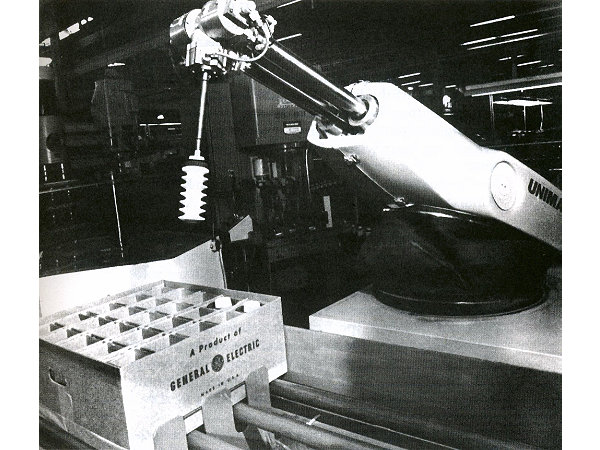
\includegraphics[height=4cm]{imgs/1_introduction/unimate.jpeg}
	\caption{Robot Unimate}
	\label{fig:unimate}
	\end{subfigure}
	\hfill
	\begin{subfigure}{0.45\textwidth}
	\centering	
	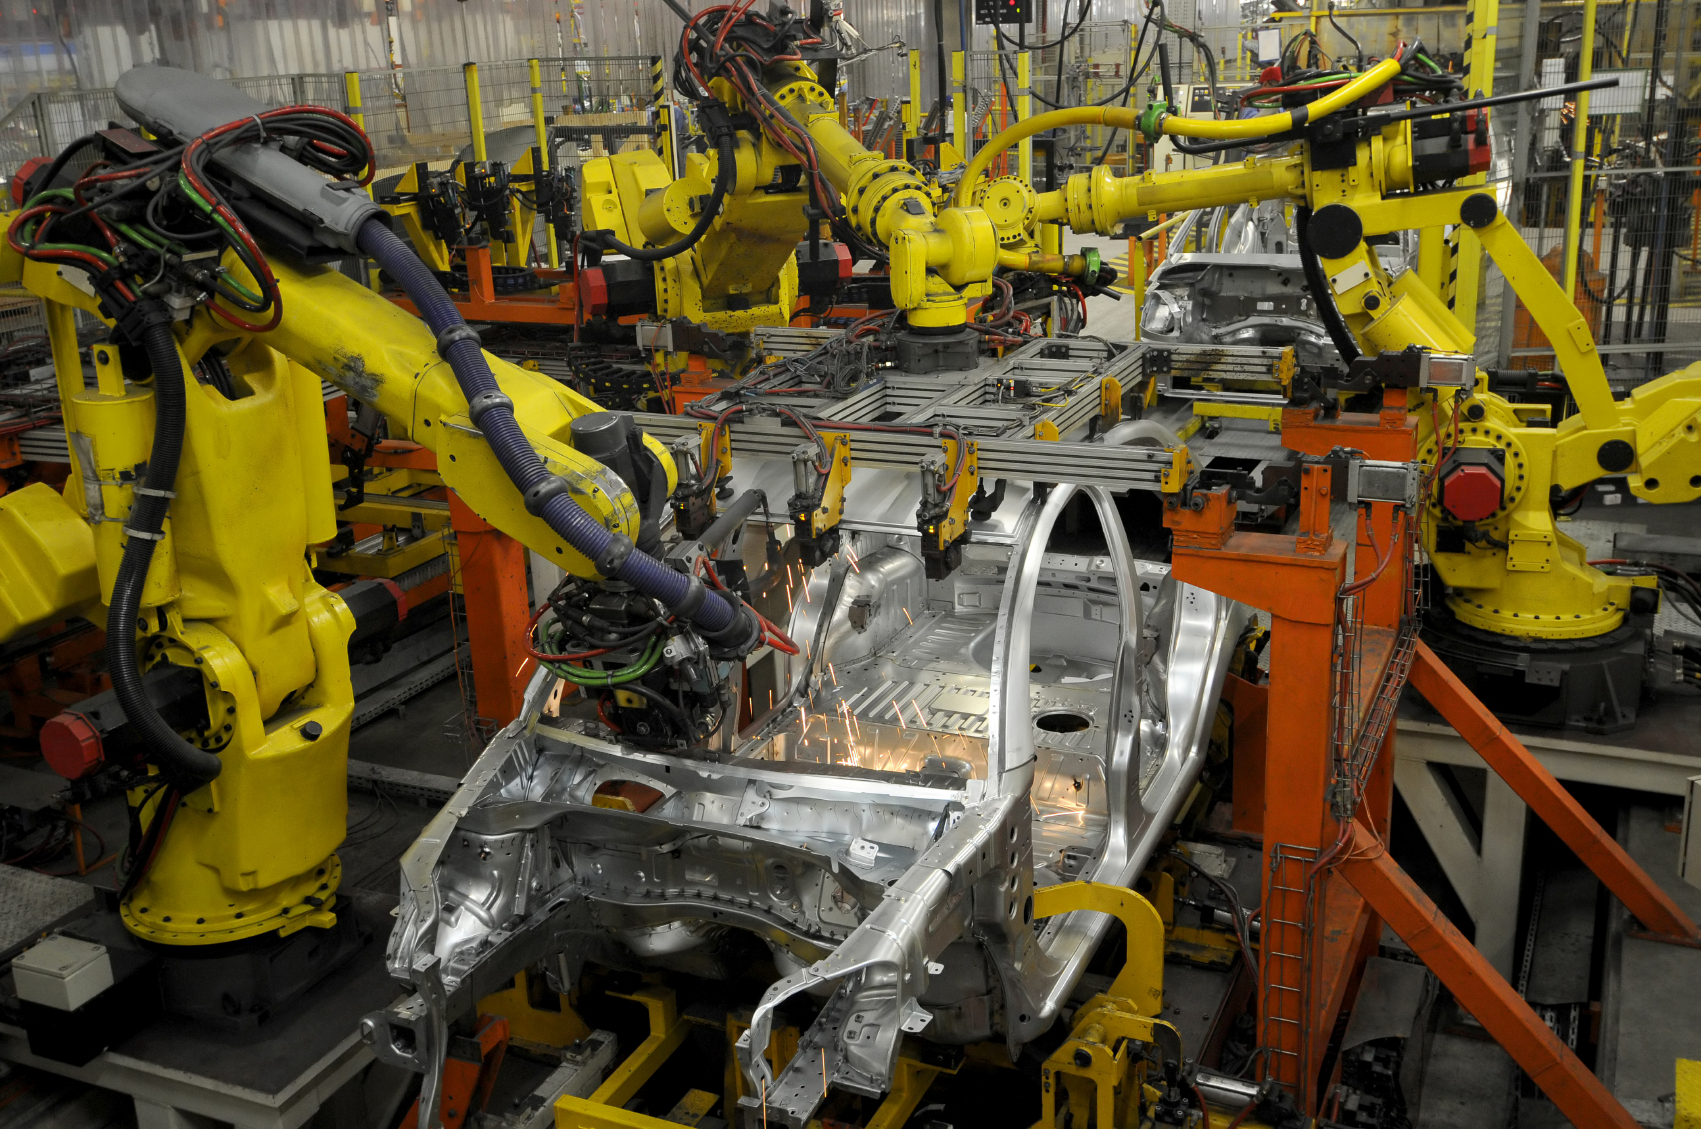
\includegraphics[height=4cm]{imgs/1_introduction/robotsCars.jpg}
	\caption{Brazos robóticos montando coches.}
	\label{fig:robotsCars}
	\end{subfigure}
\caption{Aplicaciones de robots en la industria.}
\end{figure}

Otra muestra del uso cada vez más común en la industria es el embalaje de productos, como sucede en el caso de la empresa ABB\footnote{\url{http://www.abb.es}}, dónde unos brazos robóticos dotados de visión son capaces de organizar y colocar distintos tipos de productos que van pasando delante de ellos por una cinta transportadora. \\

Otro ejemplo de aplicaciones para robots es la empresa Kiva Systems\footnote{\url{http://www.kivasystems.com}}, recientemente comprada por Amazon, el gran gigante de la venta de productos por internet. En esta empresa tienen robots encargados de mover y reubicar estanterías de varios pisos de alturas llenas de paquetes. Realizan esta tarea de manera completamente autónoma y son, además, capaces de coordinarse entre ellos para elegir la manera más óptima de realizar estos movimientos, ahorrando así una gran cantidad de recursos en la tarea (figura \ref{fig:amazonRobots}). 
	
\begin{figure}[htbp]
	\centering
	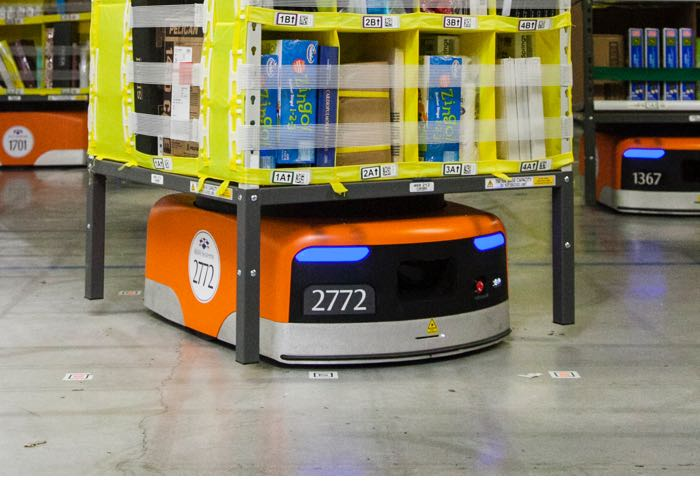
\includegraphics[height=5cm]{imgs/1_introduction/robotsAmazon.jpg}
	\caption{Robots de Amazon.}
	\label{fig:amazonRobots}
\end{figure}
	
Pero los robots no se limitan a realizar tareas industriales. También aparecen realizando actividades como limpieza de residuos tóxicos, localización y desactivación de explosivos (figura \ref{fig:robotExplosives}), búsqueda y rescate de personas, exploración de volcanes activos o fondos marinos (figura \ref{fig:robotSea}), por citar algunos ejemplos. También presentan un uso muy destacado en la exploración espacial, donde multitud de distintos robots han aportado la posibilidad de realizar misiones como la exploración de Marte mediante las sondas gemelas Spirit y Opportunity, o la construcción y mantenimiento de la ISS o EES (Estación Espacial Internacional) gracias al complejo brazo robótico ERA. \\

Otro de los campos donde el uso de robots se está haciendo cada vez más popular es la medicina, especialmente en la cirugía laparoscópica, que busca realizar las mínimas incisiones posibles. Actualmente empieza a emplearse equipamiento robótico teledirigido que permita a los cirujanos realizar operaciones muy delicadas, como por ejemplo de cirugía ocular o neurocirugía, con una precisión altísima y sin temor a que el pulso les tiemble. También se emplean robots en los laboratorios médicos para poder manejar sustancias biológicas potencialmente dañinas con el mínimo riesgo. Un claro ejemplo de estos robots es el robot "Da Vinci", creado por la empresa norteamericana Intuitive Surgical \footnote{\url{http://www.intuitivesurgical.com/}} y aprobado en el año 2000. Este sistema quirúrjico es teleoperado y se usa en múltiples procedimientos quirúrjicos con la idea de conseguir un enfoque mínimamente invasivo. Este robot puede verse en la figura \ref{fig:davinci}. \\

Observando esta gran expansión que está experimentando la robótica en campos tan diversos, no es de extrañar que actualmente también podamos encontrar robots domésticos al alcance de cualquiera. El caso más común en este ámbito es el de los robots aspiradora, actualmente comercializados por multitud de empresas, capaces de ser manejados por cualquier tipo de persona, y que gracias a sus comportamientos autónomos son capaces de limpiar pisos enteros sin necesidad de ser programados por el usuario final. Y aprovechando que hablamos de robots más económicos al alcance de todos, merece la pena mencionar que también han surgido otro tipo de robots, destinados a la generalidad del público con el fin de proporcionar entretenimiento: los robots de ocio. En los últimos años han surgido varios productos consistentes en robots que aunque técnicamente son muy avanzados si nos fijamos en los estándares de hace tan solo 30 años, no son más que “juguetes” para gran parte de la población actual. Este es el caso del robot mascota de Sony, el Robot Aibo, o el Ev3 de Lego (figura \ref{fig:ev3Lego}), un “juguete” que permite construir, programar y controlar tus propios robots. \\

\begin{figure}[htbp]
	\begin{subfigure}{0.45\textwidth}
	\centering
	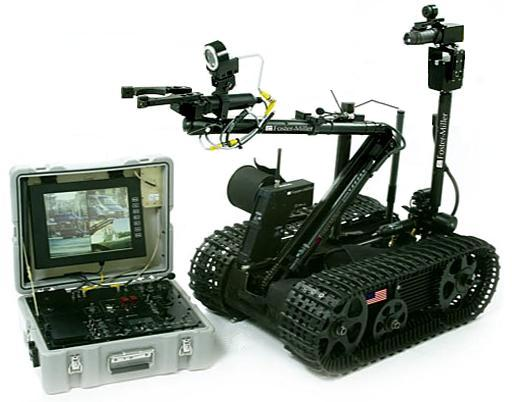
\includegraphics[height=3cm]{imgs/1_introduction/robotExplosives.jpg}
	\caption{Robot artificiero teleoperado.}
	\label{fig:robotExplosives}
	\end{subfigure}
	\hfill
	\begin{subfigure}{0.45\textwidth}
	\centering
	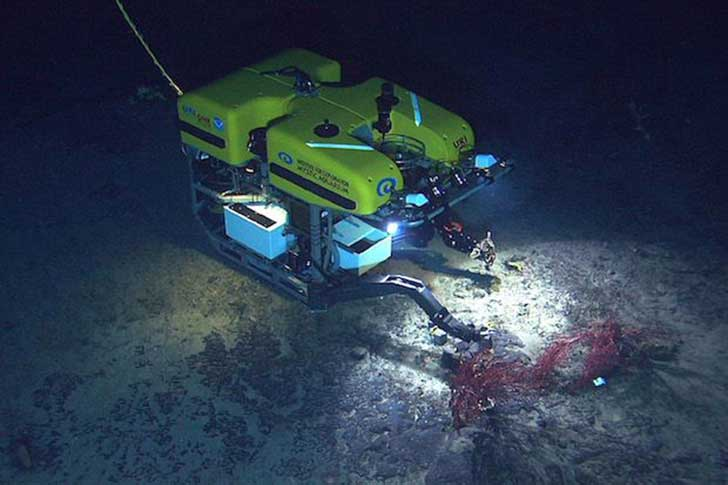
\includegraphics[height=3cm]{imgs/1_introduction/robotSea.jpg}
	\caption{Robot explorador de fondos marinos.}
	\label{fig:robotSea}
	\end{subfigure}
	\hfill
	\begin{subfigure}{0.45\textwidth}
	\centering
	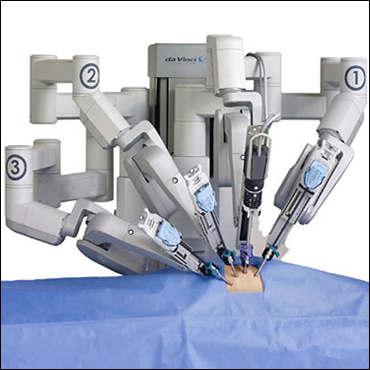
\includegraphics[height=3cm]{imgs/1_introduction/davinci.jpg}
	\caption{Robot cirujano Da Vinciteleoperado.}
	\label{fig:davinci}
	\end{subfigure}
	\hfill
	\begin{subfigure}{0.45\textwidth}
	\centering
	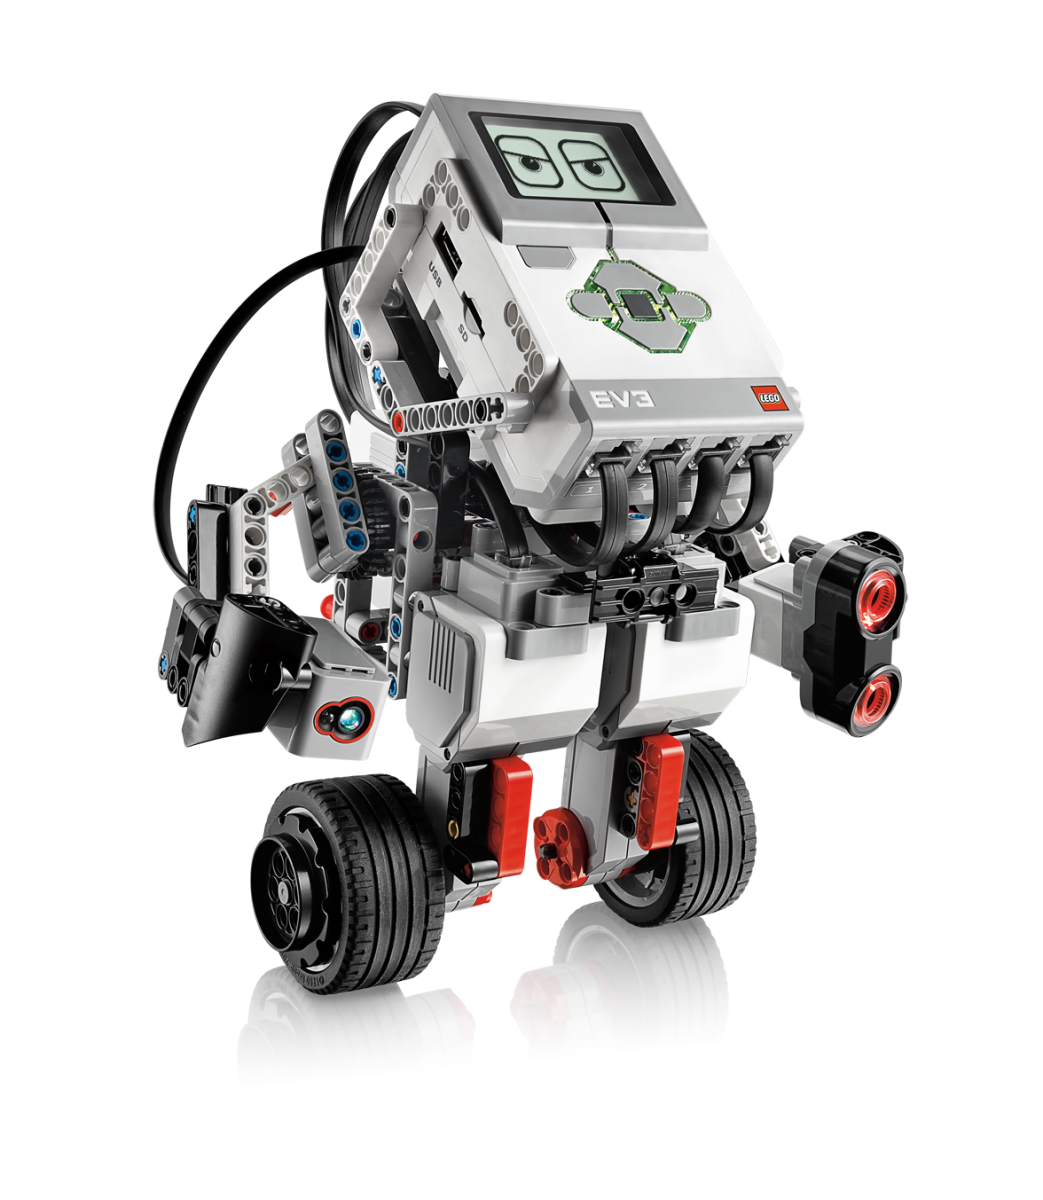
\includegraphics[height=3cm]{imgs/1_introduction/ev3Lego.png}
	\caption{Ev3 de Lego.}
	\label{fig:ev3Lego}
	\end{subfigure}
\caption{Aplicaciones de robots fuera de la industria.}
\end{figure}

Otra aplicación cada vez más extendida es el uso de UAVs (Unmanned Aerial Vehicle o vehículo aéreo no tripulado), o más comúnmente conocidos como drones. En Alemania usan este tipo de robots para vigilar los trenes, protegiéndolos así de grafiteros y vándalos. Con esta medida están ahorrar dinero, pues se estima en 10 millones de dólares anuales el gasto que supone limpiar los grafitis. Actualmente, en la Comunidad de Madrid, se está estudiando el uso de robots de este estilo, equipados con cámaras y sensores que detectan gases y agentes radiactivos, para ayudar a los servicios de emergencia en labores de rescate, reduciendo así no sólo costes económicos, sino también riesgos humanos. Además, en España, Endesa ha desplegado 14 drones equipados con cámaras de alta resolución y termográficas para revisar las líneas eléctricas. También la empresa Amazon, de la que ya hemos hablado anteriormente, ha comunicado recientemente que quiere usar drones para hacer repartos a domicilio de sus productos, llevando así el paquete hasta el comprador en el mismo día en el que éste adquirió el producto. También se está haciendo especialmente popular el uso de drones para la agricultura de precisión, dado que facilitan a los agricultores la capacidad de observar sus campos desde el aire, permitiéndoles observar las incidencias en cada campaña agrícola, ofreciendo información sobre el estado hídrico, el grado de desarrollo vegetativo y su estado sanitario en tiempo real. Ofrecen también la posibilidad de realizar riegos, fertilizaciones o tratamientos sanitarios en las zonas que los necesiten en función a la información recogida. En la figura \ref{fig:agriculturaPrecision} se puede observar un drone utilizado en este campo. Sin embargo, existen todavía muchas más aplicaciones en las que estos robots resultan útiles, como la prevención y el control de incendios, para fotografía, vídeo y cartografía aérea, buscar personas desaparecidas, etc.

\begin{figure}[htbp]
	\begin{subfigure}{0.45\textwidth}
	\centering
	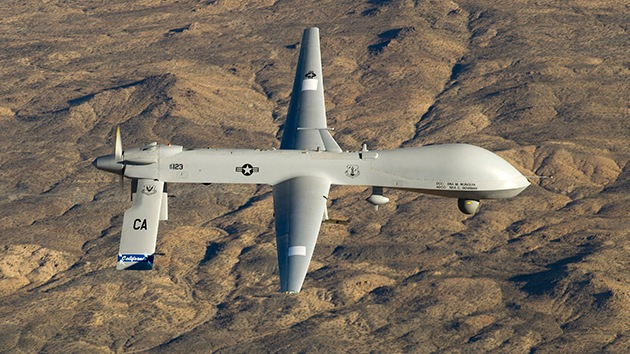
\includegraphics[height=4cm]{imgs/1_introduction/uav.jpg}
	\caption{Drone militar.}
	\label{fig:militarDrone}
	\end{subfigure}
	\hfill
	\begin{subfigure}{0.45\textwidth}
	\centering
	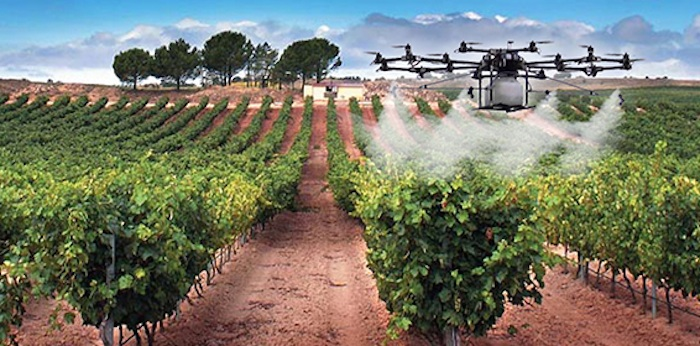
\includegraphics[height=4cm]{imgs/1_introduction/agriculturaPrecision.jpg}
	\caption{Drone en la agricultura de precisión.}
	\label{fig:agriculturaPrecision}
	\end{subfigure}
\caption{Distintos ejemplos de drones.}
\end{figure}

Otro área que se ha beneficiado de los avances de la róbotica es la industría del automóvil. Uno de los ejemplos más habituales de esta influencia son los sistemas de aparcamiento autónomo (figura \ref{fig:autoParking}), y es que cada vez son más los coches que ofrecen la posibilidad de aparcar con sólo pulsar un botón. Sin embargo, hay ejemplos más sofisticados de esta influencia, como los Model S de Tesla, que puede observarse en la figura \ref{fig:modelS}. Estos vehículos disponen de una actualización que les dotará de una función de piloto asistido y casi-automático que permitirá al conductor relajarse un rato durante las horas de más tráfico. Aunque estos coches no serán capaces de llegar autónomamente de un sitio A a otro B, son capaces de circular por la calle en la que se encuentran por si solos. Con esto nos acercamos al auténtico objetivo que se persigue con estra mezcla de robots y vehículos: los coches autónomos. Se trata de vehículos dotados de sensores e inteligencia suficiente como para conducirse por sí mismos. Aunque esta tecnología aún no está disponible, está sufriendo un gran desarrollo y una fuerte investigación y apoyo por parte de diversos sectores, destacando el fuerte impulso otorgado por Google. \\

\begin{figure}[htbp]
	\centering
	\begin{subfigure}{0.45\textwidth}
	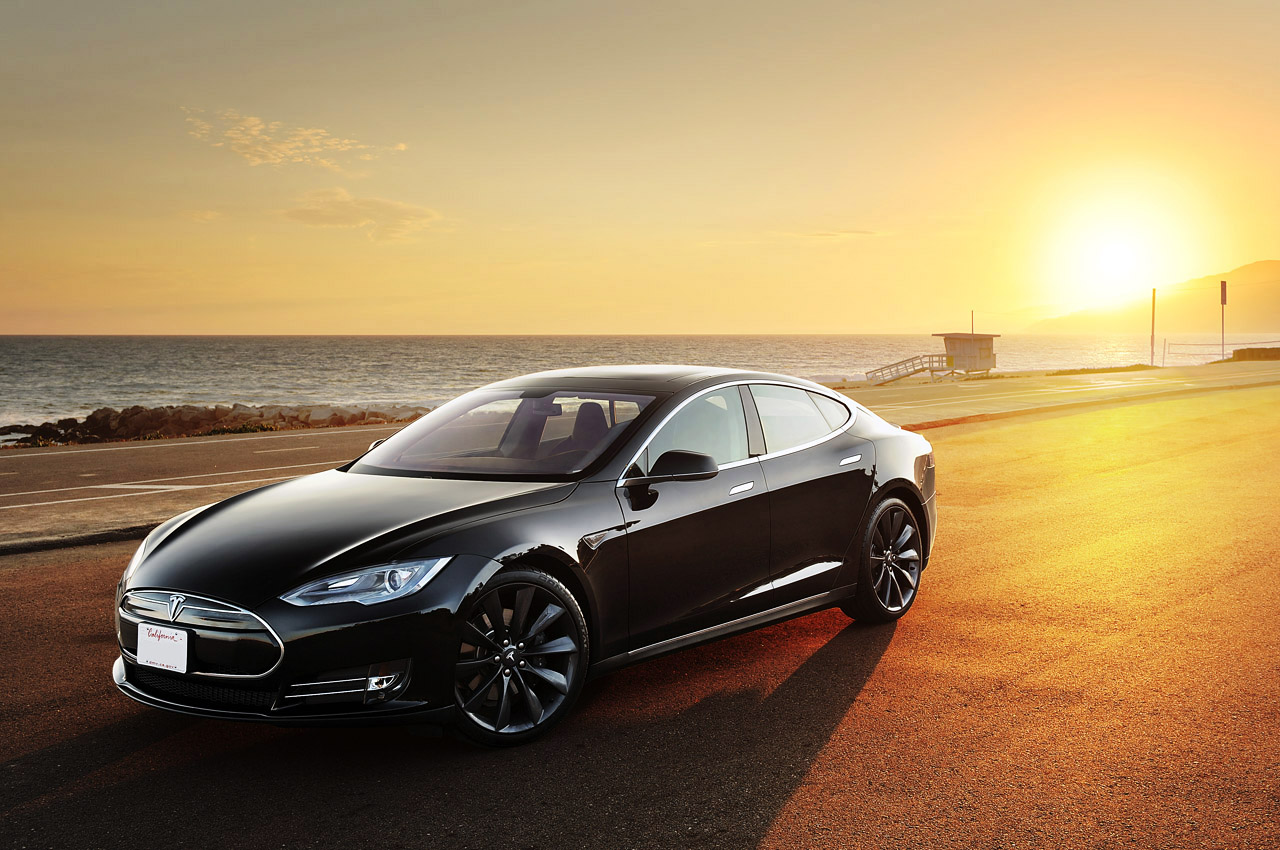
\includegraphics[height=4cm]{imgs/1_introduction/modelS.jpg}
	\caption{Model S deTesla.}
	\label{fig:modelS}
	\end{subfigure}
	\hfill
	\centering
	\begin{subfigure}{0.45\textwidth}
	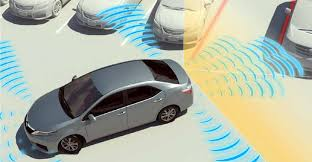
\includegraphics[height=4cm]{imgs/1_introduction/autoparking.jpeg}
	\caption{Aparcamiento autónomo.}
	\label{fig:autoParking}
	\end{subfigure}
\caption{Avances robóticos en automóviles.}
\end{figure}



En resumen, la robótica es un campo que ha sufrido una gran evolución en los últimos años, pero que aún puede evolucionar mucho más. Cada vez son más las aplicaciones comerciales robóticas, y esta tendencia continúa intensificándose. Se trata, por lo tanto, de un sector con una gran perspectiva de futuro y casi ilimitadas posibilidades y aplicaciones, que van aumentando a la vez que aumenta nuestra tecnología actual.

%%%%%%%%%%%%%%% Programación en robots %%%%%%%%%%%%%%%
\section{Programación en robots}
Ya hemos comentado el gran desarrollo que han sufrido los robots en una gran variedad de campos. Este desarrollo se debe en gran medida a su inteligencia, que no reside en los sensores encargados de captar la información del exterior o del interior propio robot, si no que radica en su software. El software es el encargado de decidir qué debe hacerse en función de toda la información que han recogido los distintos sensores. Al igual que nuestro cerebro, el software de los robots es el encargado de analizar las diversas situaciones que se le presenten, y dar una respuesta, activando los actuadores correspondientes para reaccionar de la forma más conveniente posible. La funcionalidad del robot reside fundamentalmente en su programación, en el software que maneja los recursos hardware como los sensores y actuadores.

\subsection{Plataformas}
Aunque la inteligencia de los robots reside en su software, su programación no es sencilla, principalmente debido a que no existe una metodología universal estandarizada para programar robots. Históricamente, lo único que se utilizaban eran los \textit{drivers} proporcionados por su fabricante, siendo el sistema operativo casi inexistente, consistente únicamente en una colección de \textit{drivers} con rutinas para leer valores de los sensores y escribir valores en los actuadores. Esta forma de programar se refleja en la figura \ref{fig:onDrivers}.

\begin{figure}[htbp]
	\begin{subfigure}{0.45\textwidth}
	\centering
	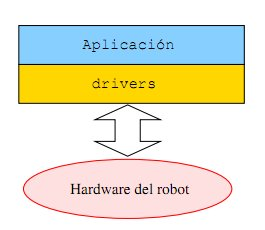
\includegraphics[height=5cm]{imgs/1_introduction/progRobots1.jpg}
	\caption{Sobre drivers de sensores y actuadores}
	\label{fig:onDrivers}
	\end{subfigure}
	\hfill
	\begin{subfigure}{0.45\textwidth}
	\centering
	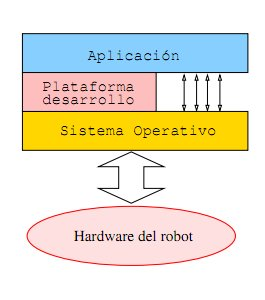
\includegraphics[height=5cm]{imgs/1_introduction/progRobots2.jpg}
	\caption{Sobre una plataforma.}
	\label{fig:onPlatform}
	\end{subfigure}
\caption{Distintos esquemas de programación de robots.}
\end{figure}

El principal problema de esta forma de desarrollar software es que resulta complicada, costosa, y, sobre todo, muy poco reutilizable. Es por esto que se hizo necesario que el desarrollo del software empezara a simplificarse, añadiendo una capa entre el sistema operativo y las aplicaciones robóticas: las plataformas de desarrollo (figura \ref{fig:onPlatform}). Añadiendo esta capa se consigue un acceso más sencillo y estandarizado a los sensores y actuadores, haciendo que a la aplicación robótica no le importe si el sensor láser que tiene el robot tiene unas características específicas u otras, ya que le ofrecerá la información en el mismo modo. \\

En los últimos años la comunidad robótica ha empezado a aplicar conceptos y metodologías de la ingeniería del software a este campo, haciendo un mayor énfasis en la reutilización del código, diseños de software distribuido, etc., y han aparecido varias plataformas de desarrollo de aplicaciones, siendo sus principales características las siguientes:

\begin{itemize}
\item Proveen de una capa de acceso al hardware (HAL, por sus siglas en inglés \textit{Hardware Access Layer}) más o menos portable.
\item Ofrecen una arquitectura de software concreta a las aplicaciones.
\item Incluyen herramientas y bibliotecas con funcionalidad lista para ser utilizada.
\end{itemize}

Muchas de estas plataformas surgidas en los últimos años estás orientadas a componentes. Son sistemas conformados en diferentes componentes lógicos o funcionales con interfaces que se usan para la comunicación entre dichos componentes. Entre estas plataformas se pueden destacar \emph{ROS}\footnote{\url{http://www.ros.org/}} (Quigley et al., 2009), \emph{Orca}  (Brooks et al., 2007, Makarenko et al., 2006), \emph{Microsoft Robotics Studio}, \emph{RoboComp} y \emph{JdeRobot} (Cañas Plaza, 2003), entre otras.

\subsection{Lenguajes Visuales}
Como se explica en \cite{borja2014}, existen también diferentes formas de programar un robot. La primera de ellas consiste en escribir directamente su código fuente, pudiendo utilizarse lenguajes como Java, C/C++ o Python, entre otros, igual que en la programación de cualquier otra aplicación informática. Lo que hace que un lenguaje pueda ser usado para programar robots son las bibliotecas que estén desarrolladas para él. \\

A parte de estos lenguajes “tradicionales” de programación, ha habido intentos de crear lenguajes específicos para programar robots que contasen con primitivas propias de la robótica. En este tipo de lenguajes se encuentran los \textit{Taks Descrition Language} (TDL) o \textit{Reaction Active Packages} (RAP). Pero lo que realmente se puede considerar un avance en la programación específica es el surgimiento de los \emph{lenguajes de programación visual} (LPV). Estos lenguajes se caracterizan por utilizar únicamente elementos gráficos para programar, de forma que no es necesario introducir código escrito “a mano”, como se hace tradicionalmente. Este tipo de lenguajes ofrecen una programación muy intuitiva y didáctica, pudiéndose observar además de manera muy clara  aspectos esenciales en un programa informático, como el flujo de ejecución, sus condiciones, bucles, etc. En resumen, podríamos definir un LPV como:

\begin{itemize}
\item Un lenguaje de programación que utiliza una representación visual como gráficos, dibujos, iconos o animaciones.
\item Un lenguaje que manipula información visual o soporta interacción visual, o permite programar utilizando expresiones visuales.
\item Un conjunto de símbolos de texto y gráficos con una interpretación semántica que es utilizada para comunicar acciones en un entorno.
\item Lenguaje de programación donde se usan técnicas visuales para expresar relaciones o transformaciones en la información.
\end{itemize}

Hay que aclarar que un LPV no es un entorno integrado de desarrollo (IDE). La diferencia es que un LPV debe ser capaz de llevar a cabo todas las tareas de programación de forma visual, sin tener que recurrir a la representación textual. \\

Entonces, ¿por qué insistimos en comunicarnos con los ordenadores y las máquinas mediante lenguajes de programación textuales? ¿No sería mejor hacerlo mediante una programación que aproveche nuestra naturaleza visual? Los autores de los LPV discuten que la respuesta a esta pregunta es sí, siendo algunas de las principales motivaciones:

\begin{itemize}
\item Mucha gente piensa y recuerda cosas en términos de esquemas y cuadrados.
\item Las personas nos relacionamos con el mundo de forma intrínsecamente gráfica y utilizamos imágenes como el componente primario del pensamiento creativo.
\end{itemize}

Sin embargo, los LPV también presentan algunas limitaciones, siendo la más importante que, al no poder introducir código textualmente, el programador se encuentra limitado a utilizar los recursos que éste le brinde. \\

Un ejemplo muy ilustrativo de LPV en robótica es el lenguaje RCX de Lego. Fue creado inicialmente para niños, caracterizándose por su simplicidad y legibilidad. Se empleó para la programación de su juguete RCX, siendo utilizado más tarde también en su evolución, el NXT. Estaba pensado para poder ser utilizado por niños, y consta de bloques visuales que representan acciones o condiciones, permitiendo, mediante el apilamiento de dichos bloques, componer un comportamiento más o menos complejo de  manera sencilla. Mediante estos bloques puede lograrse que el robot se mueva, emita un sonido, o reaccione a distintos eventos. En la figura \ref{fig:lego} se puede ver el aspecto de este lenguaje.

\begin{figure}[htbp]
	\centering
	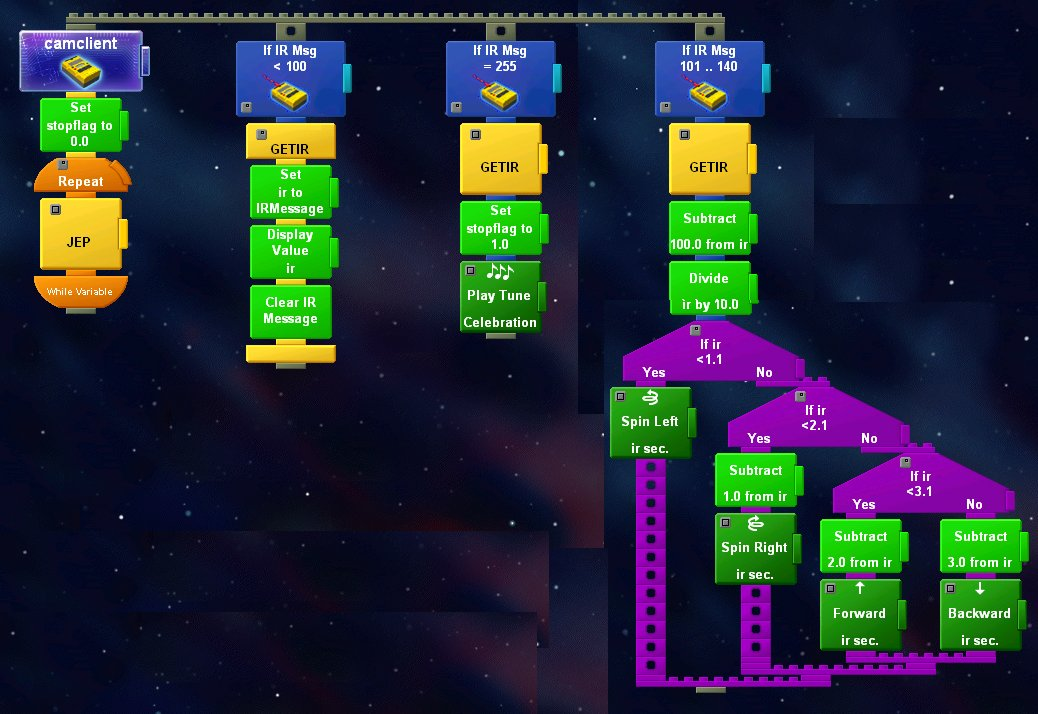
\includegraphics[height=6cm]{imgs/1_introduction/rcxCode.jpg}
	\caption{Imagen RCX code de Lego.}
	\label{fig:lego}	
\end{figure}

Otro de los puntos fuertes de los LPV es que, gracias a su aspecto fácilmente legible, se convierten en elementos didácticos ideales, permitiendo así un primer y sencillo contacto para los niños con el mundo de la programación. Aunque no tengan que escribir código directamente, estos lenguajes les permiten acostumbrarse y empezar a entender distintas estructuras empleadas en la programación, como los condicionales o los bucles, entres otros. Precisamente dentro de este enfoque entran los dos ejemplos que vamos a citar a continuación: \emph{Scratch} y \emph{Blockly}. \\

\emph{Scratch}\footnote{\url{https://scratch.mit.edu/}}\cite{scratchEducativo} es un lenguaje pensado para que los pequeños aprendan a pensar de forma creativa, razonar de forma sistemática, y además, tengan un primer contacto con la programación. Este lenguaje permite programar historias interactivas, juegos, animaciones, y compartirlos con los demás en la comunidad online. Y, por supuesto, toda la programación se realiza de forma visual, concatenando distintos bloques, tal y como podemos ver en la figura \ref{fig:scratch}. \\

\emph{Blockly}\footnote{\url{https://developers.google.com/blockly/}}\cite{learningWithBlockly} es una librería de JavaScript que también utiliza bloques para programar. Es un proyecto open source de Google similar a Scratch que apareció por primera vez en 2012. Esta librería está siendo ampliamente utilizada sobre todo para aplicaciones educativas como \textit{Blockly Games}\footnote{\url{https://blockly-games.appspot.com/?lang=es}}, pero no reduciéndose a este campo, dado que también está siendo utilizado como IDE para desarrollar aplicaciones para Android, entre otros usos. Si observamos la figura \ref{fig:blockly} podremos ver un ejemplo resuelto de uno de los distintos juegos educativos que se ha hecho con esta librería. \\

\begin{figure}[htbp]
	\centering
	\begin{subfigure}{0.49\textwidth}
	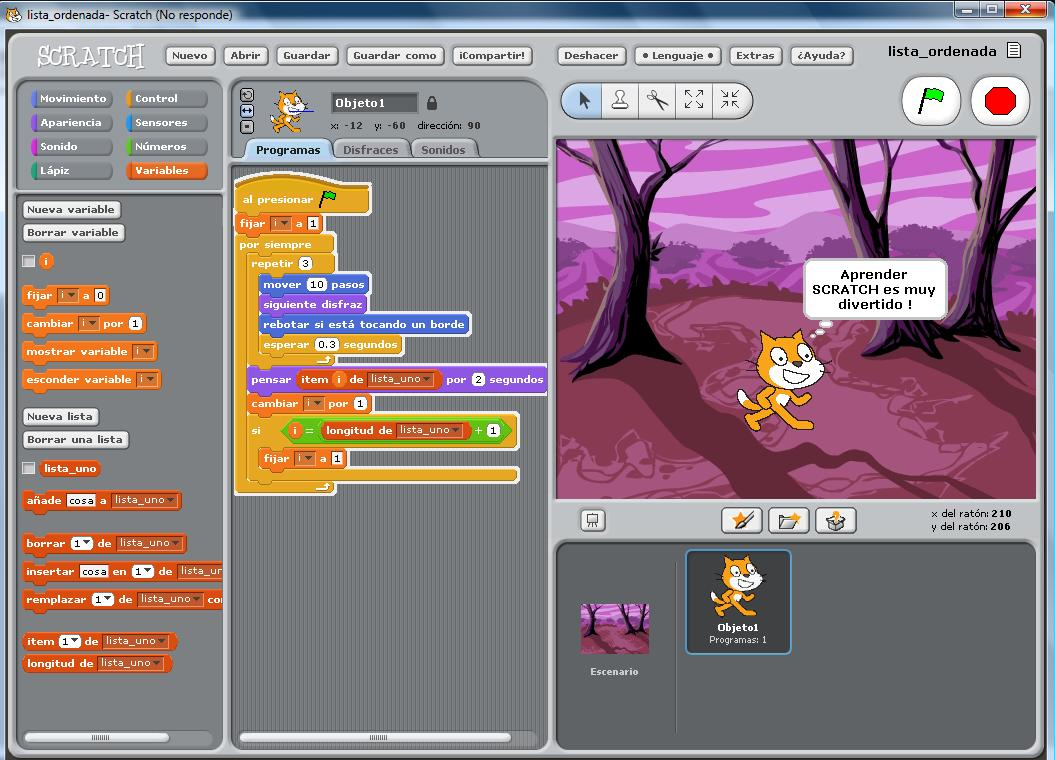
\includegraphics[height=6cm]{imgs/1_introduction/scratch.jpg}
	\caption{Ejemplo de uso de Scratch.}
	\label{fig:scratch}
	\end{subfigure}
	\hfill
	\centering
	\begin{subfigure}{0.49\textwidth}
	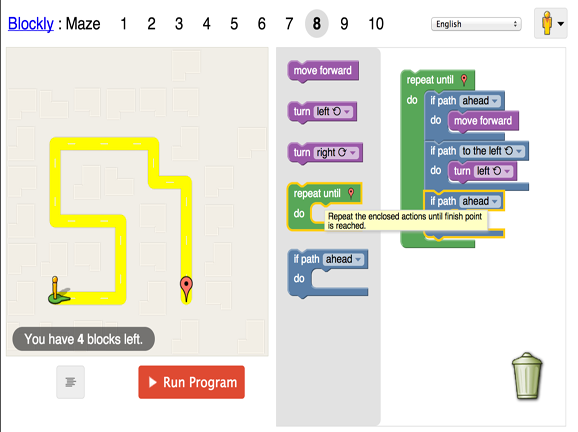
\includegraphics[height=6cm]{imgs/1_introduction/blockly.png}
	\caption{Ejemplo de uso de Blockly.}
	\label{fig:blockly}
	\end{subfigure}
\caption{Aplicaciones educativas de los LPV.}
\end{figure}

\subsection{Autómatas}
Los autómatas finitos o Máquinas de Estado Finito (FSM, \textit{Finite State Machines}) se han utilizado exitosamente para representar comportamientos de robots\cite{foukarakis2014combining}, representándolos de manera compacta y abstracta. Con estos autómatas el comportamiento es representado mediante un conjunto de \textit{estados}, cada uno de los cuales está encargado de realizar una tarea particular. El sistema puede cambiar de un estado a otro mediante \textit{transiciones}, que son las condiciones de cambio que dependen de ciertos eventos o cambios producidos en los sensores del robot, ya sean internos o externos. \\

Los autómatas de estados finitos ofrecen una forma inteligente y sencilla de organizar el código de control y de percepción dentro de un robot móvil. Han sido explorados en investigación y también incorporados en plataformas de desarrollo robóticas recientes, con herramientas que le dan al programador la capacidad de abstraerse un poco más de los detalles de la implementación y centrarse en la lógica del comportamiento que está interesado en programar. De esta forma, la mayor parte del código es autogenerado en base al comportamiento programado, lo que hace disminuir en gran medida la aparición de errores y reducir el tiempo de desarrollo de forma considerable, permitiendo, además, programar comportamientos complejos de forma robusta. \\

\begin{figure}
	\centering
	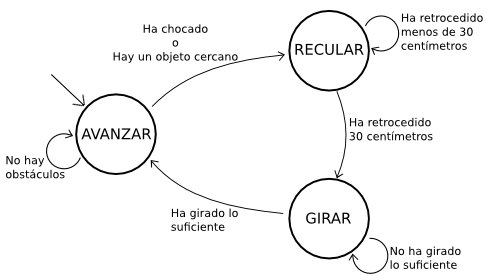
\includegraphics[height=5cm]{imgs/1_introduction/AutomataRobot.jpg}
	\caption{Ejemplo de autómata que define un comportamiento sencillo para un robot.}
	\label{fig:simpleAutomata}
\end{figure}

Conviene añadir también, que esta forma de representar el comportamiento de los robots utilizando autómatas de estado finito combina a la perfección con el uso de un LPV, o, al menos, con una aproximación más gráfica que los lenguajes de programación puramente textuales, dado que el flujo de control puede ser perfectamente representado gráficamente mediante un esquema de estados y transiciones, tal cómo hemos se ve en la figura \ref{fig:simpleAutomata}. \\

Una herramienta comercial que utiliza programación visual en base a autómatas jerárquicos es \textit{XaitControl}, de la empresa Xaitment, empleada en videojuegos para programar la inteligencia artificial de los jugadores automáticos. Como se aprecia en la figura \ref{fig:xaitControl}, este programa cuenta con una zona principal donde se pinta el autómata, una vista lateral que muestra toda la estructura creada, y otros paneles con distintas informaciones sobre procedimientos auxiliares, control de flujo de ejecución, etc.  Esta herramienta cuenta además con ciertas características muy avanzadas, como por ejemplo la capacidad de diseñar un autómata finito no determinista (AFND). Un AFND es un autómata en el que, por ejemplo, se pueda transitar por dos caminos diferentes entre un estado origen y un estado final. Permite también la creación de proyectos compuestos por uno o varios autómatas jerárquicos cada uno, pudiendo ver todas las dependencias existentes entre ellos gracias a la vista en forma de árbol. Cuenta con un compilador que le permite lanzar la aplicación programada, utilizando la misma interfaz para ver los progresos, pudiendo establecer puntos de parada en el flujo de ejecución, avance instrucción a instrucción y otras funcionalidades comunes a cualquier depurador. \\

\begin{figure}
	\centering
	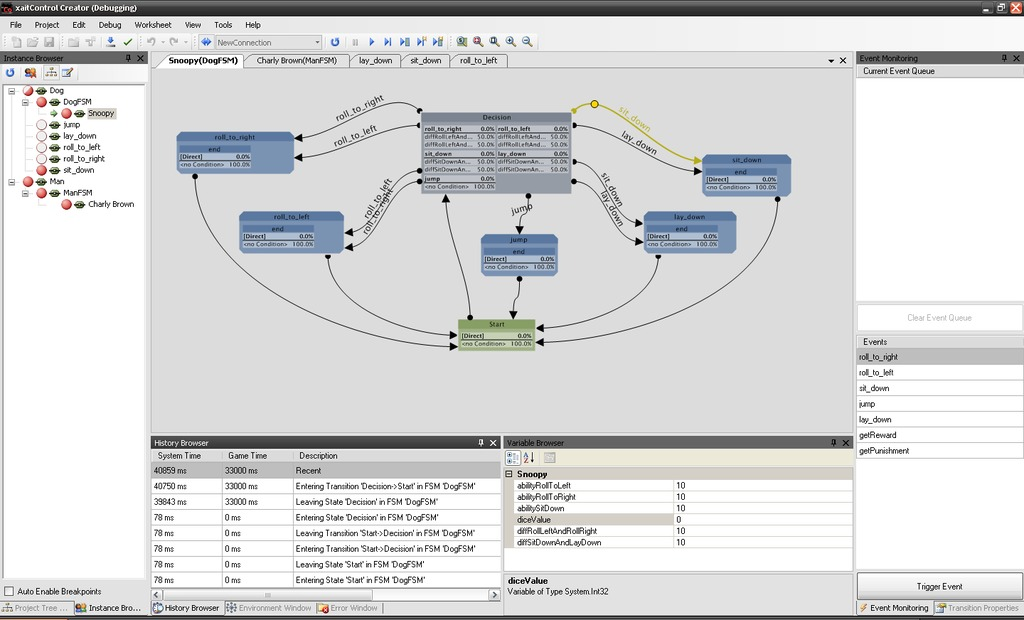
\includegraphics[height=5cm]{imgs/1_introduction/xaitControl.jpg}
	\caption{Captura de XaitControl.}
	\label{fig:xaitControl}
\end{figure}

Otra herramienta que utiliza esta aproximación de autómatas finitos es \textit{SMACH}\footnote{\url{http://www.ros.org/wiki/smach}}\cite{bohren2011towards, smach2013}, una herramienta de la plataforma ROS que consiste en una arquitectura a nivel de tarea que permite crear comportamientos complejos para robots de forma rápida. En su núcleo, SMACH es una librería de Python que permite construir máquinas de estado finito jerárquicas. Para esto, hay que escribir el código  necesario para crear y describir cada estado y transición, por lo que no puede considerarse un LPV, dado que la programación no se realiza de forma gráfica sino introduciendo el código. Sin embargo, esta librería viene también con el \textit{SMACH viewer} (figura \ref{fig:smach}), una herramienta que muestra la máquina de estados desarrollada en tiempo de ejecución, de forma que podemos ver el gráfico o la vista de árbol de nuestro autómata aunque no los dos a la vez. También muestra todos los estados y transiciones, así como aquellos que estén activos y una ventana de ayuda dónde se pueden ver los datos relativos a este estado activo. \\

\begin{figure}
	\centering
	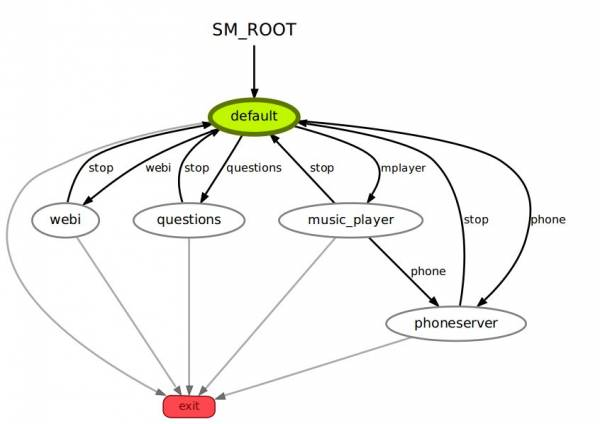
\includegraphics[height=5cm]{imgs/1_introduction/smach.jpg}
	\caption{Captura de SMACH viewer.}
	\label{fig:smach}
\end{figure}

Actualmente, herramientas similares a estas que acabamos de describir están siendo ampliamente utilizadas en la programación de Inteligencia Artificial (IA), especialmente para adversarios en los videojuegos. Vemos con esto que estas herramientas no tienen por qué estar ligadas necesariamente a robots, si no que tienen más aplicaciones. \\

\begin{figure}[htbp!]
	\centering
	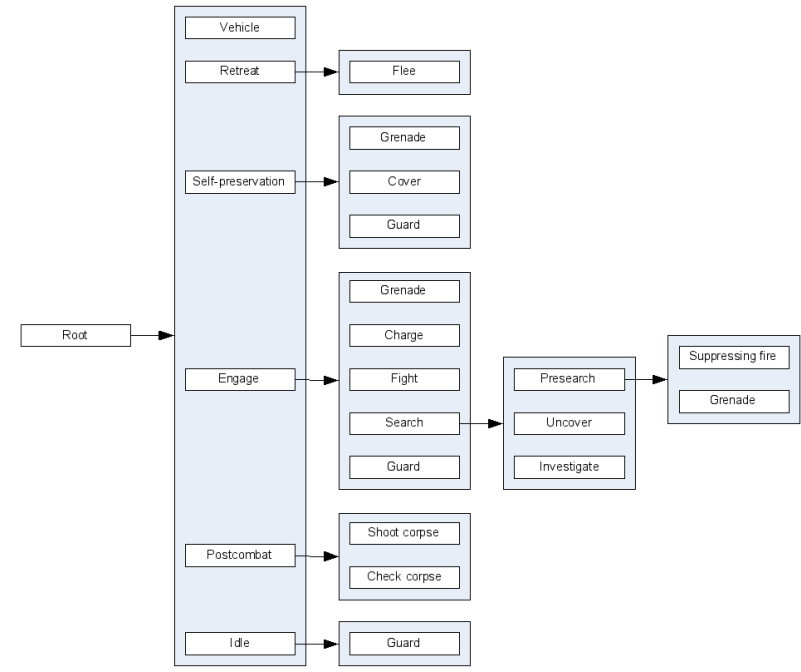
\includegraphics[width=11.5cm]{imgs/1_introduction/halo_2.png}
	\caption{Ejemplo de autómata del videojuego Halo 2.}
	\label{fig:halo2}
\end{figure}

En la figura \ref{fig:halo2} se puede observar un comportamiento programado mediante un autómata finito y jerárquico, similar a los que hemos estado describiendo. Este ejemplo proviene del videojuego Halo 2, y representa la inteligencia de los jugadores automáticos. Cada acción del primer nivel despliega uno o más niveles, especializando con cada paso las acciones a ejecutar. \\

\enspace
Con estos temas principales en los que hemos centrado esta sección, las plataformas, los LPV, y el uso de autómatas finitos para la programación del comportamiento, hemos introducido los dos pilares fundamentales sobre los que se apoya nuestra herramienta, VisualHFSM, de la que hablaremos a continuación.

%%%%%%%%%%%%%%% VisualHFSM %%%%%%%%%%%%%%%
\section{VisualHFSM}
Para terminar con este capítulo de introducción, vamos a hablar a continuación de la herramienta de la plataforma JdeRobot en la que se centra este TFG: VisualHFSM (\textit{Visual Hierarchy Finit State Machine}). VisualHFSM es una herramienta que combina ventajas de los LPV y del uso de las máquinas de estados finitos jerárquicos para desarrollar el comportamiento de robots de forma sencilla, haciendo que el desarrollador tenga que preocuparse de programar sólo el código imprescindible. Para crear un autómata bastará con \textit{dibujar} los estados y transiciones que van a definir su comportamiento en la ventana del editor gráfico. Esto definirá el flujo de control del autómata, y, a continuación, se puede añadir el código que se desee que se ejecute en cada estado o en las transiciones. \\

Se puede usar el editor gráfico además para generar el archivo de configuración necesario para conectar el componente creado con sus interfaces ICE (lo explicaremos más adelante), si se desean incluir librerías adicionales, e incluso compilar el autómata mediante CMake\footnote{\url{https://cmake.org/}}, también generado automáticamente. El proyecto se guardará utilizando un archivo XML, en el que se escribirán todos los datos necesarios para reconstruirlo a la hora de abrirlo para seguir trabajando con él. Todo esto se materializa en código que el autómata ejecuta en rápidas iteraciones periódicas, comprobando en cada iteración en que estado se encuentra, si se debe transitar o no a otro estado, y ejecutando el código del estado correspondiente. La velocidad con la que estas iteraciones se producen  también puede modificarse mediante VisualHFSM. \\

Es importante tener en cuenta que esta no es una herramienta nueva creada en este TFG, sino que proviene de la evolución que ha ido sufriendo a lo largo de los años durante sus diferentes versiones. Es un proyecto complejo y potente que ha sufrido un largo proceso de maduración para llegar a su estado actual. \\

La primera versión de esta herramienta fue desarrollada por Carlos Iván\footnote{\url{http://jderobot.org/Cmartin-pfc-itis}} en su TFG\cite{martin2010herramienta} en el año 2010. Todavía no recibió el nombre de VisualHFSM y fue el primer acercamiento desarrollado en la Universidad Rey Juan Carlos dentro de la plataforma JdeRobot, siendo compatible con su versión 4.3. Permitía la programación de robots mediante autómatas mononivel que funcionaban sobre el componente básico de dicha versión. Contaba con todo lo esencial para diseñar los autómatas de estado finito de manera visual y autogenerar código en C, incluyendo una versión inicial de la GUI y cómo guardar el proyecto en un archivo XML. \\

La siguiente versión de esta herramienta la realizó David Yunta\footnote{\url{http://jderobot.org/Dyunta-pfc-itis}} en el año 2011\cite{yunta2012herramienta, paperDavidYunta}], y su principal mejora introducida fue la migración de la aplicación a a nueva versión de JdeRobot, la 5.0. Esta versión de VisualHFSM nos permitía seguir desarrollando autómatas mononivel y generaba el código inspirado en el componente \textit{Introrob}, también perteneciente a la misma plataforma. Contaba con una interfaz gráfica nueva y con una gran mejora en los componentes generados, dado que éstos incluían una GUI en tiempo de ejecución. Esta GUI mostraba los estados por los que el robot iba transitando a medida que ejecutaba su comportamiento programado. Esto era una poderosa característica que facilitaba mucho las tareas de depuración del código, permitiendo controlar en todo momento si el robot se estaba comportando como el desarrollador esperaba que lo hiciese. Además, el código que generaba la aplicación era C++. \\

Visual HFSM 3.0\cite{salamanques2012} fue realizada por Rubén Salamanqués\footnote{\url{http://jderobot.org/Rubensb-pfc-itis}} en el año 2012. Con esta versión Rubén dotó a la herramienta de mayor poder, al hacer posible que trabajase con autómatas jerárquicos, permitiendo que dentro de un estado pudiese haber subautómatas. Con esto se consiguió que la herramienta sirviese para programar comportamientos más complejos de una manera más sencilla. La única pega que esta mejora tuvo fue que supuso la pérdida de la GUI en tiempo de ejecución, pues esta GUI sólo estaba planteada para soportar autómatas mononivel. El código que generaba también era C++ y seguía siendo compatible con la versión de JdeRobot 5.0. \\

La cuarta y última versión hasta la fecha, VisualHFSM 4.0\cite{borja2014, menendezprogramming}, fue desarrollada por Borja Menéndez\footnote{\url{http://jderobot.org/Bmenendez-tfm}}. Las principales mejoras son que incluyó ejemplos usando el robot \textit{Nao}, mientras que hasta ahora sólo se había podido usar VisualHFSM con el robot \textit{Pioneer}. Además renovó la GUI, haciendo que el canvas para dibujar el autómata fuese más espacioso y añadió el \textit{Tree View}, donde se podía ver la representación textual del autómata entero, mostrando sus distintos subniveles debajo de su nodo padre para ver todos los estados del autómata, algo muy útil para trabajar con autómatas multinivel. Sin embargo, la herramienta seguía sin recuperar la GUI en ejecución.

\begin{figure}[htbp]
	\begin{subfigure}{0.4\textwidth}
	\centering
	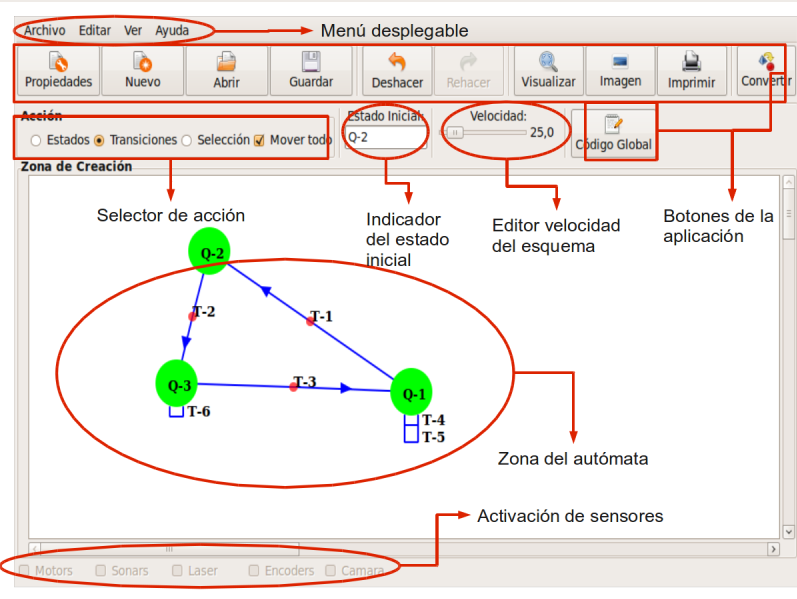
\includegraphics[height=4cm]{imgs/1_introduction/visualHFSM1.png}
	\caption{VisualHFSM 1.0}
	\label{fig:visualHFSM1}
	\end{subfigure}
	\hfill
	\begin{subfigure}{0.4\textwidth}
	\centering
	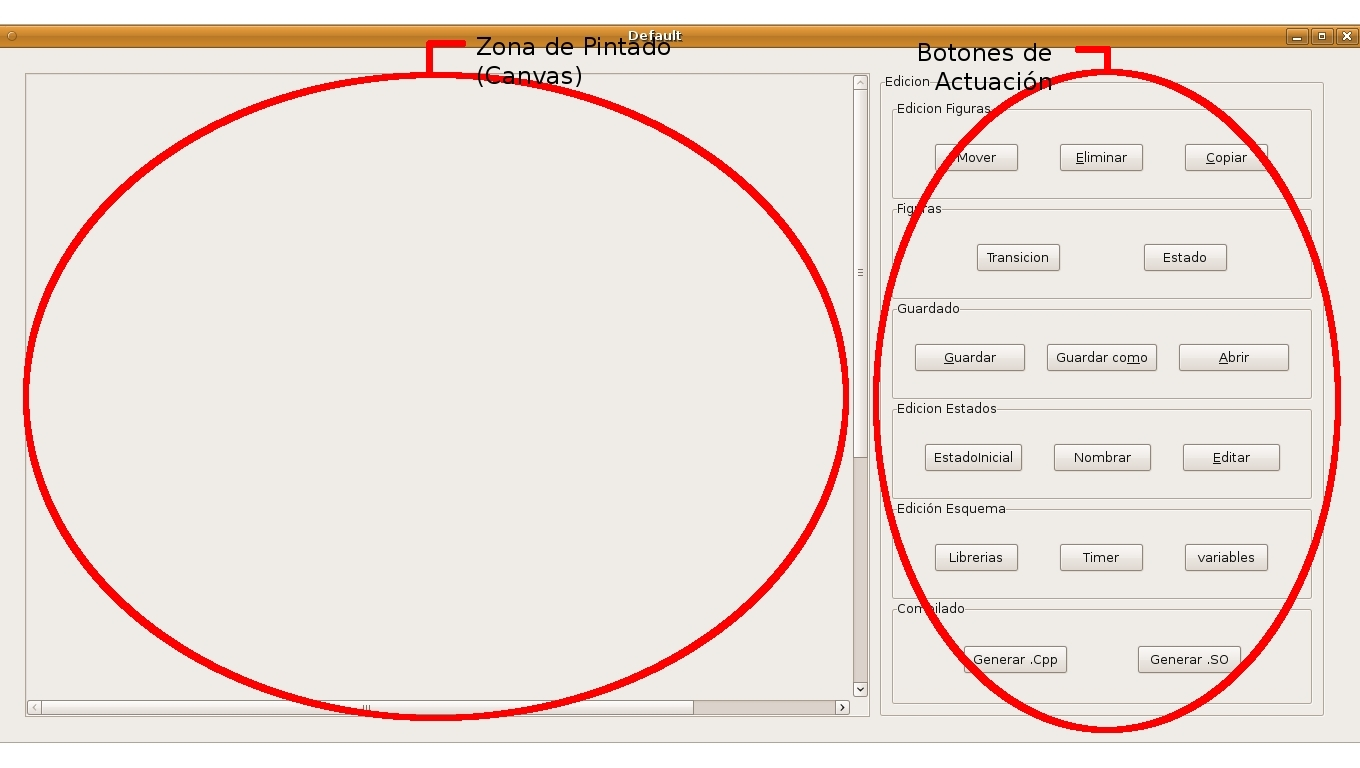
\includegraphics[height=4cm]{imgs/1_introduction/visualHFSM2.jpg}
	\caption{VisualHFSM 2.0}
	\label{fig:visualHFSM2}
	\end{subfigure}
	\hfill
	\begin{subfigure}{0.4\textwidth}
	\centering
	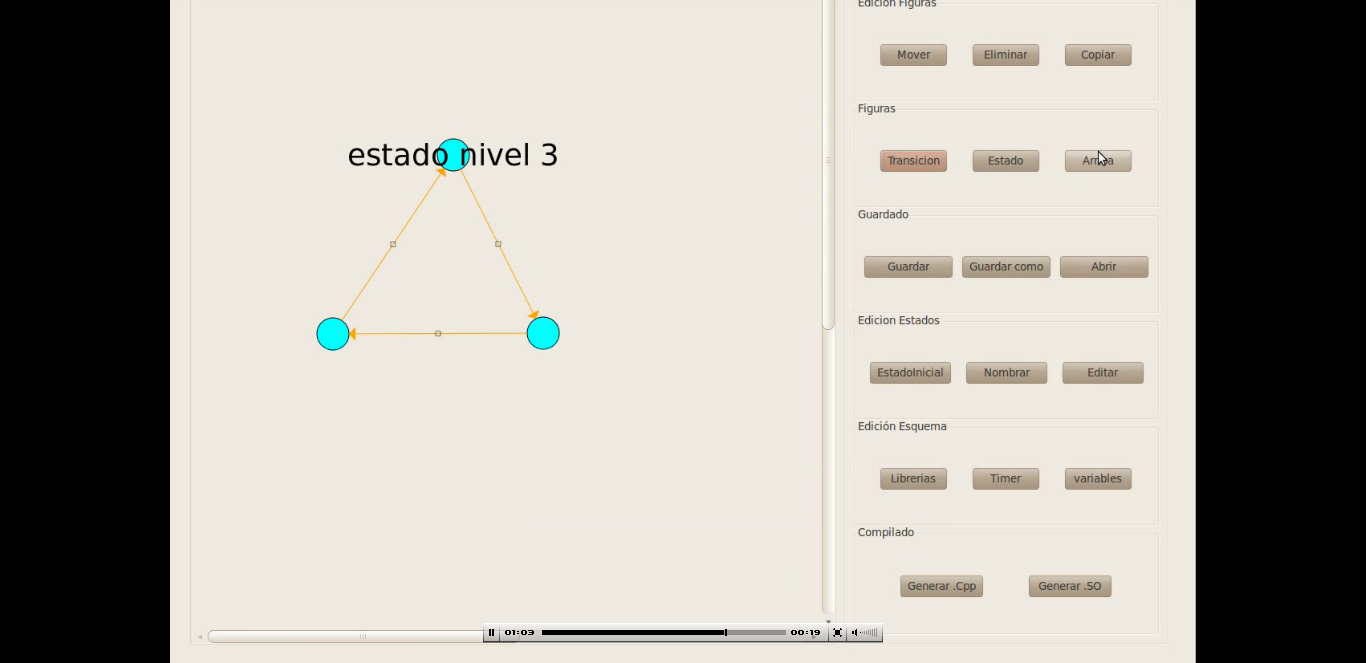
\includegraphics[height=4cm]{imgs/1_introduction/visualhfsm3.png}
	\caption{VisualHFSM 3.0}
	\label{fig:visualHFSM3}
	\end{subfigure}
	\hfill
	\begin{subfigure}{0.4\textwidth}
	\centering
	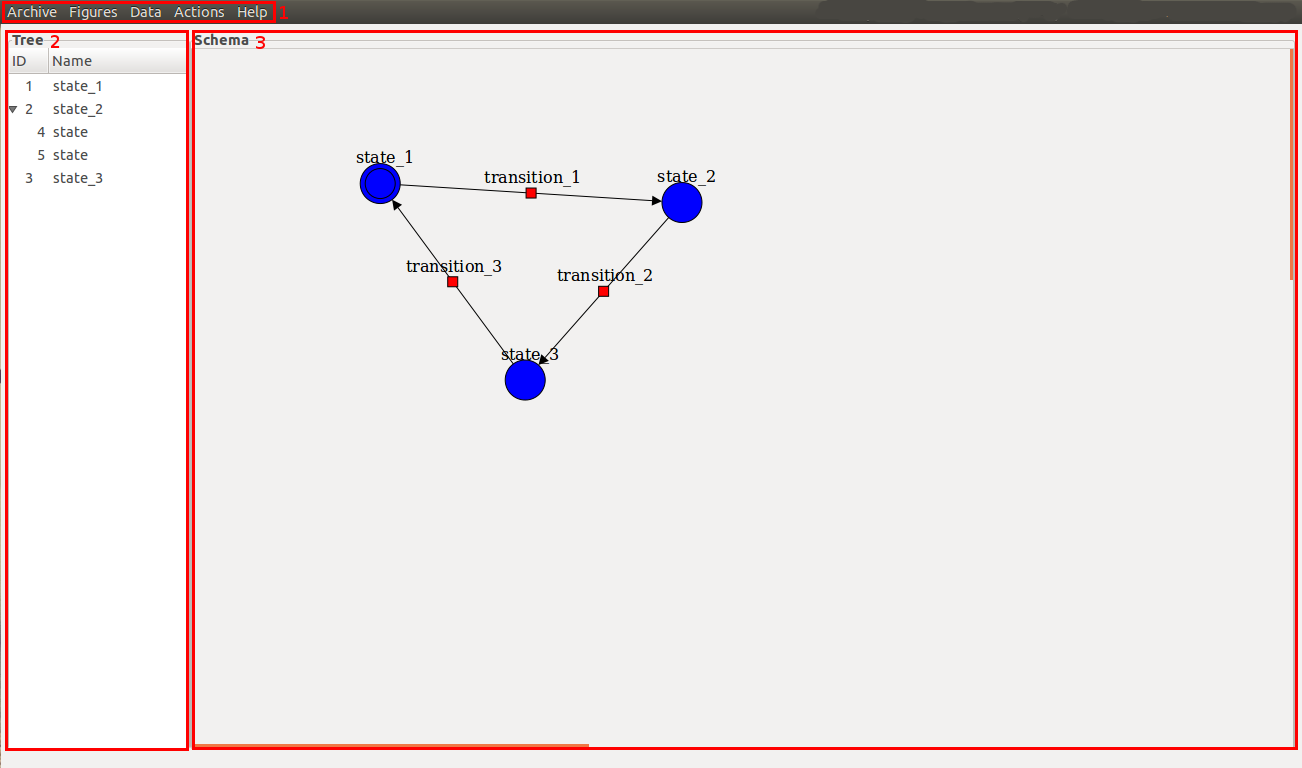
\includegraphics[height=4cm]{imgs/1_introduction/visualHFSM4.png}
	\caption{VisualHFSM 4.0}
	\label{fig:visualHFSM4}
	\end{subfigure}
\caption{Evolución de la GUI a lo largo de las distintas versiones de VisualHFSM}
\label{fig:visualHFSMGUIs}
\end{figure}

A la hora de ejecutar los autómatas creados por esta herramienta hay que tener en cuenta que, desde que soportan jerarquía, es un código \textit{multi-hilo}, dado que cada subautómata supone un hilo de ejecución distinto. El componente generado está preparado para soportar esto, pero si el código que se inyecta en los estados y transiciones es sensible a las condiciones de carrera, el programador deberá ser consciente de esta situación y utilizar las medidas necesarias para solventarlo. Aunque, cómo acabamos de explicar, hay un hilo de ejecución por cada subautómata, no todos están activos a la vez. Cada hilo sólo está ejecutando el código de su estado activo y comprobando si tiene que transitar a otros estados cuando su padre está activo. En caso contrario, el hilo estará esperando a que su padre se active sin hacer nada. \\

En cuánto al hilo de ejecución que sigue cada subautómata, la idea es sencilla. En un primer lugar entra en un \textit{switch-case} de control. Aquí cada subautómata se encarga de evaluar si su padre está activo (en caso de tenerlo), y de ser así, comprueba cuál es su estado activo, y si se cumple alguna de las condiciones necesarias para que se active una de sus transiciones. Si éste es el caso, se ejecutará el código de la transición (en caso de haberlo), y se pondrá como estado activo de este subautómata el nuevo estado. En caso de que no sea necesario realizar ninguna transición, el estado activo seguirá siendo el mismo. A continuación, hay un \textit{switch-case} de acción. Ahora, si el padre está activo, se comprueba cuál es el estado actual y se ejecuta su código. Todo esto se encuentra dentro de un bucle infinito, y se repite periódicamente en función de la frecuencia que el programador haya establecido mediante el editor.

\vspace{1.5cm}
En el segundo capítulo describiremos los objetivos concretos y fijaremos los requisitos que debe cumplir esta nueva versión de VisualHFSM a desarrollar en este proyecto. En el capítulo de infraestructura se analizarán en detalle las herramientas software que se han empleado. En el cuarto capítulo describiremos de forma detallada las soluciones que se han programado para conseguir los objetivos propuestos. En el siguiente, comprobaremos experimentalmente el funcionamiento de la estructura conseguida, montando distintos comportamientos para drones, todos generados con VisualHFSM 5.0. Por último, esta memoria terminará describiendo las conclusiones a las que hemos llegado, y las posibles líneas futuras de trabajo a partir de este proyecto.
\chapter{Objetivos}\label{chap:Objetivos}
Tras haber presentado en el capítulo anterior el contexto general del proyecto, con sus motivaciones, y los dos pilares principales sobre los que se apoya, nos disponemos a fijar sus objetivos, sus requisitos mínimos, y el plan de trabajo para llevarlo a cabo.

%%%%%%%%%%%%%%% Descripción del problema %%%%%%%%%%%%%%%
\section{Descripción del problema}
El objetivo general de este proyecto es conseguir una versión mejorada de la herramienta VisualHFSM, que sea lo suficientemente madura como para ser utilizada cómodamente por terceros. \\

Al dar a conocer la herramienta pretendemos que los desarrolladores de aplicaciones robóticas descubran una potente herramienta que puede ahorrarles tiempo al permitirles programar el comportamiento de robots de forma más rápida y sencilla utilizando una representación de estados y transiciones. Además, nos servirá para saber cómo es percibida la herramienta por los usuarios, recibir realimentación y descubrir nuevas formas de mejorar aún más su usabilidad, para conseguir una aplicación lo más cómoda y amigable posible. \\

VisualHFSM seguirá siendo una herramienta que se aproxima a los LPV, con una interfaz gráfica que permitirá programar el comportamiento del autómata mediante un diagrama de estados, reduciendo al mínimo el código que el usuario necesita introducir. \\

Para conseguir esto, hemos separado el problema en varios subobjetivos:

\begin{itemize}
\item \textbf{Mejorar la usabilidad del editor gráfico}: Aunque el editor gráfico ya está bastante maduro, aún tiene aspectos que conviene mejorar, como la navegación entre niveles o la flexibilidad al crear archivos de configuración. Además, nos hemos encontrado con algunos errores que perjudican la usabilidad de la herramienta.
\item \textbf{Recuperar la GUI en ejecución para autómatas multinivel}: Esta característica permite visualizar en tiempo de ejecución qué estados están activos, actualizándose éstos dinámicamente. Aunque esta funcionalidad resulta muy útil para la depuración de los componentes, se perdió cuando se añadió soporte para autómatas \textit{jerárquicos} en anteriores versiones de VisualHFSM, y con esta versión nos hemos propuesto como objetivo recuperar dicha funcionalidad.
\item \textbf{Generar componentes en Python}: Con el fin de incrementar la flexibilidad que VisualHFSM ofrece, otro de los objetivos es añadir la posibilidad de generar componentes en Python, además del generador de código C++ ya existente. Es importante que también pueda utilizarse la GUI en ejecución para estos componentes.
\item \textbf{Difusión}: Además de centrarnos en mejorar la herramienta, también consideramos necesario realizar un esfuerzo en cuanto a su difusión, dándola a conocer a la comunidad robótica y facilitando su uso.
\end{itemize}


%%%%%%%%%%%%%%% Requisitos %%%%%%%%%%%%%%%
\section{Requisitos}
Tras haber explicado los objetivos propuestos, los requisitos de partida a los que deberá ajustarse el proyecto son:

\begin{itemize}
\item La herramienta no puede perder funcionalidad ya existente.
\item Tiene que ser capaz de representar gráficamente el autómata en tiempo de ejecución de forma que sea fácilmente comprensible.
\item La GUI en tiempo de ejecución debe soportar una gran número de estados, transiciones y subautómatas, permitiendo una navegación cómoda entre ellos.
\item Cuando el autómata se genere con código Python, VisualHFSM debe mantener todas las funcionalidades que tenía para autómatas de C++. Estas funcionalidades incluyen el GUI en tiempo de ejecución.
\item El código generado debe ser compatible con la plataforma robótica \emph{JdeRobot 5.3.2.}
\end{itemize}

%%%%%%%%%%%%%%% Plan de trabajo %%%%%%%%%%%%%%%
\section{Metodología y plan de trabajo}
El desarrollo de este proyecto seguirá el modelo en espiral, basado en la necesidad de separar el comportamiento final en varias subtareas más sencillas que luego se juntarán. Cada tarea finalizada aporta los requisitos y la información necesaria para abordar la siguiente iteración del modelo de desarrollo, creándose además puntos de control cada vez que se finaliza una de estas tareas. \\

Además, durante toda la realización del proyecto se mantendrán reuniones con el tutor cada semana o cada dos semanas, con el fin de monitorizar los avances obtenidos, el estado global del proyecto, y plantear nuevos objetivos. Así mismo, todos los logros y avances se registrarán y comentarán en la MediaWiki\footnote{\url{http://jderobot.org/S.rey-tfg}}, pudiendo encontrarse el código en mi repositorio de GitHub\footnote{\url{https://github.com/reysam93/TFG}}, el cuál se irá actualizando. \\

El desarrollo de este TFG seguirá los siguientes pasos:
\begin{enumerate}
\item \textbf{Familiarización con la plataforma JdeRobot y el simulador Gazebo:} Empezaremos el proyecto con la instalación de la plataforma JdeRobot y sus dependencias, probando distintos componentes simples y haciéndoles pequeñas modificaciones para jugar un poco con el entorno y acostumbrarnos a él.

\item \textbf{Familiarización con VisualHFSM:} VisualHFSM es una herramienta compleja que cuenta con una gran cantidad de código. Crearemos comportamientos sencillos para robots utilizando la versión existente para ver cómo se comporta, detectar posibles flecos a mejorar, y comprender su código fuente.

\item \textbf{Realización del GUI en en tiempo de ejecución para C++:} Tras tener claro como funciona la herramienta, nos encargaremos de utilizar GTK+ y Glade para diseñar la GUI en tiempo de ejecución, que debe ser lo más similar posible al editor gráfico. Para esto, primero se elaborará la GUI en tiempo de ejecución para autómatas mononivel, y después para autómatas jerárquicos, siendo necesario modificar el generador de código para que cree un hilo adicional que relacionado con el GUI en tiempo de ejecución, que añadirá a la plantilla el código necesario para actualizar el estado en el que se encuentra el autómata.

\item \textbf{Generador de código en Python:} Crearemos un nuevo generador automático de código en Python que utilizará una nueva plantilla y creará el autómata siguiendo un modelo de programación orientado a objetos.

\item \textbf{GUI en tiempo de ejecución para Python:} Esta vez, se creará con PyQt4 y contará con alguna funcionalidad adicional que no está disponible en la GUI de C++. Su realización seguirá el mismo planteamiento que en C++: primero se realizará para autómatas mononivel y después para autómatas jerárquicos.

\item \textbf{Realización de experimentos:} Para comprobar el correcto funcionamiento de las mejoras introducidas, todo el proceso irá acompañado de la realización de experimentos simples, creando algún escenario más complejo para la validación final.

\item \textbf{Crear una documentación detallada:} Una vez que la herramienta esté lista, será necesario crear una documentación fácil y clara para que los usuarios interesados en utilizar la herramienta tengan un primer contacto lo más sencillo posible.
\end{enumerate}


\chapter{Infraestructura}\label{chap:Infraestructura}
En este capítulo vamos a hablar de la infraestructura que da soporte a este proyecto, y las diversas herramientas que se han utilizado para realizarlo. Para esto, empezaremos explicando qué es JdeRobot, la plataforma en la que se enmarca VisualHFSM. A continuación, hablaremos de Gazebo y comentaremos la importancia de los simuladores en robótica. Después detallaremos qué es ICE, y finalizaremos comentando las distintas librerías gráficas utilizadas para elaborar la GUI, principalmente GTK+ y PyQt4, y la herramienta Glade.

%%%%%%%%%%%%%%% JdeRobot %%%%%%%%%%%%%%%
\section{JdeRobot}
Inicialmente la plataforma JdeRobot\footnote{\url{http://jderobot.org}}\cite{peredadocencia, canas2013recent} fue creada como resultado de una tesis doctoral, y ha sido mantenida y mejorada a largo de los años por el laboratorio de Robótica de la Universidad Rey Juan Carlos, un grupo voluntario de desarrolladores.  \\

JdeRobot es una plataforma de código libre pensada para facilitar la programación de aplicaciones de robótica y visión artificial. Es una plataforma orientada a componentes, con distintos elementos independientes. Estos componentes se ejecutan siguiendo un modelo cliente-servidor, en el que cada aplicación es ejecutada como un proceso, ofreciendo una interfaz para programar sistemas de tiempo real y resolver problemas que estén relacionados con la sincronización de procesos y la adquisición de datos. Tradicionalmente, los componentes estaban principalmente programados en C/C++, aunque en la actualidad la tendencia es utilizar el lenguaje Python. Sin embargo, hay programas en otros lenguajes, como por ejemplo, JavaScript. \\

JdeRobot simplifica el acceso a los sensores y actuadores (a los dispositivos hardware), permitiendo obtener valores y enviar datos de forma sencilla. Para esta interacción, utiliza como puente los interfaces de comunicación ICE. \\

Por último, comentar que todo el código y los componentes que se encuadran en esta plataforma puede encontrarse en GitHub\footnote{\url{https://github.com/RoboticsURJC/JdeRobot}}. La arquitectura se encuentra dividida en componentes, drivers, interfaces, librerías y herramientas. VisualHFSM se sitúa dentro de esta plataforma en la sección de herramientas, y es compatible con su última versión, JdeRobot 5.3.2.


%%%%%%%%%%%%%%% Gazebo %%%%%%%%%%%%%%%
\section{Gazebo}
A pesar de que la robótica es un campo que genera un gran interés, en ocasiones, la gran inversión necesaria para acceder al hardware puede resultar prohibitiva. Es por esto que la simulación por ordenador se plantea como una alternativa válida y de bajo coste. Sin embargo, la simulación ofrece otras ventajas adicionales que justifican su uso:

\begin{itemize}
\item \textsl{Gestión de recursos:} Utilizar un simulador combinado con una capa de abstracción al hardware (HAL), permite desarrollar código para robots existentes pero a los que no se tiene acceso en un determinado momento. Esto resulta especialmente útil cuando hay varios desarrolladores trabajando con un único robot.
\item \textsl{Control del tiempo:} Algunos simuladores (entre ellos, Gazebo), permiten modificar el tiempo, parándolo o acelerándolo, tanto negativa como positivamente. Esto resulta especialmente útil, por ejemplo, a la hora de hacer pruebas de durabilidad o para inspeccionar el estado de los robots en cierto momento.
\item \textsl{Prototipado:} Gracias a la simulación existe la posibilidad de crear software para robots que aún no han sido contruidos.
\item \textsl{Reusabilidad:} Como el uso de simuladores suele combinarse con algún tipo de capa de abstracción, el código generado puede ser compartido con otras personas.
\end{itemize}

Gazebo\footnote{\url{www.gazebosim.org}} es un simulador 3D que ofrece un entorno para desarrollar y probar sistemas multirrobot de manera sencilla\cite{koenig2004design}. Permite la simulación realista de gran variedad de sensores y actuadores como cámaras, láser, GPS, etc., gracias, en parte, al motor de física que utiliza, ODE (\textit{Open Dynamics Engine}), y a la librería gráfica OpenGL (\textit{Open Graphics Library}). Además, Gazebo da soporte a una gran variedad de robots comerciales como \emph{Turtlebot}, el \emph{Pioneer 2-DX} o el \emph{Ar Drone}, y es también una herramienta de software libre. \\

Este simulador nació dentro del proyecto Player/Stage, pero se acabó separando y está siendo mantenido por Open Source Robotics Foundation\footnote{\url{http://www.osrfoundation.org/}}, una empresa de I+D sin ánimo de lucro e independiente encargada de apoyar el desarrollo, la distribución y la adopción del código abierto en investigación con robots, educación y desarrollo de productos. Además, Gazebo ha recibido financiación de DARPA (\textit{Defense Advanced Research Projects Agency}), convirtiéndose así en el simulador estándar \textit{de facto} dentro de la comunidad robótica, siendo empleado también para el \textit{DARPA Robotics Challenge}. \\

Otra de las principales características de Gazebo es que permite crear nuevos modelos y mundos robóticos. Un mundo simulado en Gazebo es un conjunto de todos los modelos y factores ambientales, como al luz o la gravedad. Los modelos se componen de al menos un cuerpo, con las articulaciones que éste pueda necesitar. Cuando el modelo está listo, las aplicaciones robóticas se conectan al simulador mediante los \textit{plugins} o bibliotecas dinámicas. Es necesario implementar estas bibliotecas utilizando la API de Gazebo. En la figura \ref{fig:gazeboWorld} podemos observar uno de los mundos de Gazebo creados para un experimento.

\begin{figure}[htbp]
	\centering
	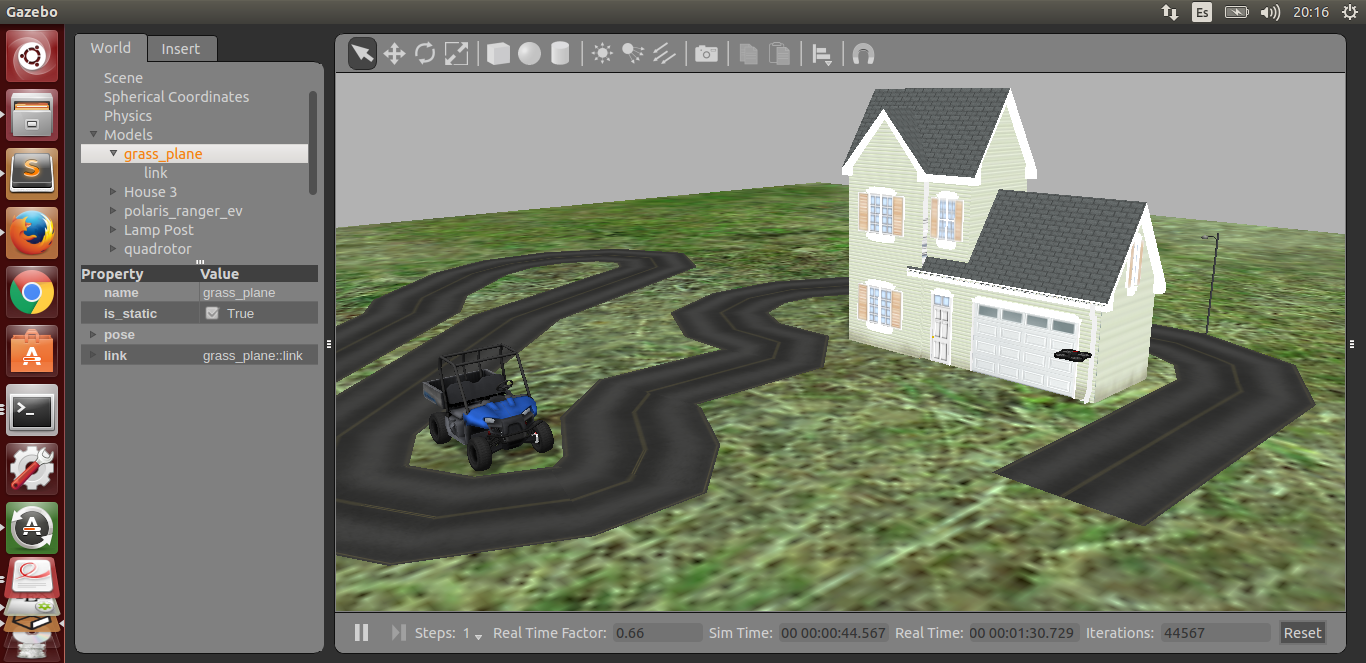
\includegraphics[height=7cm]{imgs/3_infrastructure/gazeboWorld.png}
	\caption{Mundo de Gazebo creado para realizar pruebas.}
	\label{fig:gazeboWorld}
\end{figure}

En este TFG hemos utilizado Gazebo 5.3 para simular los mundos de los experimentos y los robots que han ejecutado los componentes generados mediante VisualHFSM para comprobar su correcto funcionamiento.

%%%%%%%%%%%%%%% ICE %%%%%%%%%%%%%%%
\section{ICE}
ICE\footnote{\url{https://zeroc.com/}} es un \textit{middleware} desarrollado por ZeroC empleado por JdeRobot para la intercomunicación de componentes, especialmente importante para comunicarse con los \textit{drivers} que permiten la relación con los sensores y actuadores del robot. Es un entorno RPC (\textit{Remote Procedure Call}) orientado a objetos que provee de una capa de abstración sobre la red y sus conexiones, con una doble licencia GNU GPL y una licencia propietaria. \\

ICE permite utilizar aplicaciones de Internet sin la necesidad de usar los protocolos HTTP, y además, es capaz de atravesar cortafuegos, una característica que lo diferencia de la mayoría de los \textit{middleware} similares. Soporta  distintos sistemas operativos como Windows, MAC OS X, Linux y Solaris, y provee un IDE (\textit{Interface Definition Language}): SLICE (\textit{Specification Language for ICE}), que ayuda a definir la manera de comunicación y los parámetros utilizados entre los componentes. Una vez que dicho interfaz de comunicación está definido, se puede compilar en distintos lenguajes, dando así soporte a Python, C++, C\#, Java o JavaScript, entre otros. Además, esto hace que el cliente y el servidor puedan estar programados en distintos lenguajes. \\

Existe también una variante, ICE-E, que permite utilizar ICE dentro de teléfonos móviles. \\

Para nuestra herramienta hemos utilizado ICE 3.6 para que los componentes generados con VisualHFSM puedan comunicarse con los sensores y actuadores del robot.


%%%%%%%%%%%%%%% GTK+, Glade %%%%%%%%%%%%%%%
\section{GTK+}
Para la realización de este proyecto hemos utilizado diferentes librerías gráficas para diseñar la GUI en tiempo de ejecución. Para el componente generado en C/C++ hemos empleado la tercera versión de \emph{GTK+}. El principal motivo por el que hemos empleado esta librería, ha sido porque queríamos que el aspecto de la GUI en tiempo de ejecución fuese lo más parecido posible a la GUI del editor gráfico, y con la idea también de reutilizar y reestructurar todo el código posible del editor. \\

GTK+\footnote{\url{http://www.gtk.org}} o \textit{TheGIMP ToolKit} es un conjunto de bibliotecas multiplataforma que permiten desarrollar interfaces gráficas de usuario (GUI, \textit{Graphic User Interface}). GTK es una interfaz orientada a objetos para programadores de aplicaciones (API, \textit{Application Programming Interface}), escrita principalmente en C, aunque cuenta con enlaces a otros lenguajes de programación como C++, Python y C\#. \\

GTK+ se basa en las bibliotecas desarrolladas por el equipo de GTK+ y por el equipo de GNOME\footnote{\url{http://www.gnome.org}}:

\begin{itemize}
\item \textbf{GLib:} Se trata de una biblioteca de bajo nivel que envuelve la mayor parte de las funciones de la biblioteca estándar de C para manejar estructuras de datos, portabilidad, interfaces para funcionalidades de tiempo de ejecución como ciclos, hilos de carga dinámica o un sistema de objetos.
\item \textbf{GDK:} Es una biblioteca que actúa como intermediaria entre gráficos de bajo nivel y gráficos de alto nivel.
\item \textbf{ATK:} Una biblioteca que permite la creación de interfaces accesibles para gente discapacitada.
\item \textbf{Pango:} Permite el diseño y renderizado de texto, siendo esta biblioteca el núcleo para mejorar las fuentes y el texto en GTK+2.
\item \textbf{Cairo:} Biblioteca de renderizado avanzado de controles de aplicación.
\item \textbf{GTK:} La biblioteca principal que contiene los objetos y funciones necesarios para crear e interaccionar con la interfaz de usuario.
\end{itemize}

Con GTK+ cada elemento de la interfaz gráfica recibe el nombre de \textit{Widget}. Los \textit{widgtets} pueden representar botones, cuadros de diálogos, barras de deslizamiento, etc. Existe una gran multitud de \textit{widgets} distintos, pero todos ellos heredan de una misma clase, tal como se observa en la figura \ref{fig:treeViewHeritage}, en la cual podemos observar el esquema de herencia de la clase Gtk::TreeView.

\begin{figure}[htbp]
	\centering
	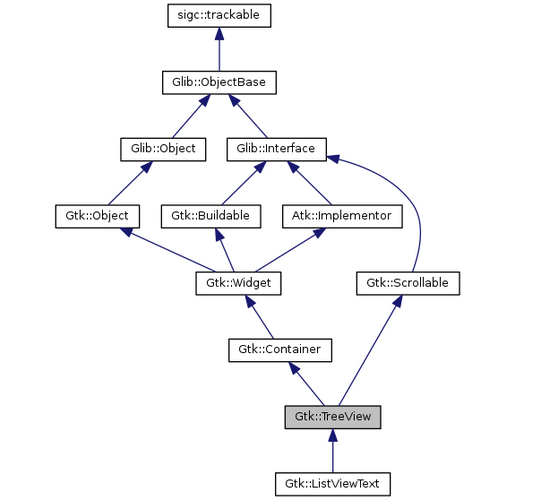
\includegraphics[height=6cm]{imgs/3_infrastructure/herenciaTreeView.png}
	\caption{Esquema de la herencia de la clase Gtk::TreeView.}
	\label{fig:treeViewHeritage}
\end{figure}

La forma de  interactuar con los \textit{widgets} es utilizando eventos. Cuando tiene lugar un evento, como hacer click en un \textit{widget} o cerrar una ventana, se emitirá una señal concreta. Esta señal puede ser conectada a una función (\textit{manejador} o \textit{callback}), de forma que cuando se emita dicha señal, se activará su manejador y se ejecutará el código que se haya programado dentro de él. De esta forma, para realizar una acción concreta cuando se pulse un botón, sólo es necesario programar dicha acción dentro de una función, y conectar la señal con ella. \\

\begin{figure}[htbp]
	\centering
	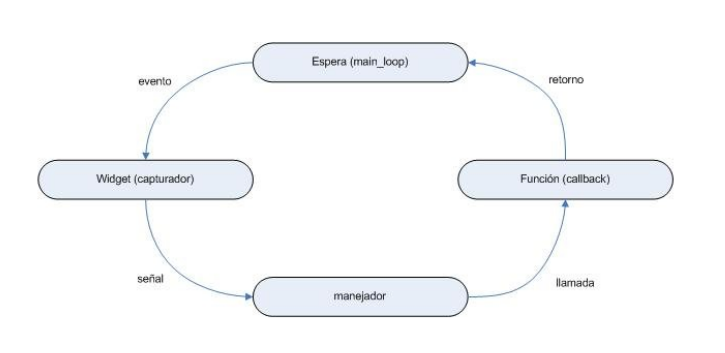
\includegraphics[height=6cm]{imgs/3_infrastructure/bucleGTK.png}
	\caption{Diagrama de flujo de GTK+.}
	\label{fig:gtkMain}
\end{figure}

Al trabajar con eventos, el diagrama de flujo de una aplicación GTK+ es como el que se observa en la figura \ref{fig:gtkMain}. Una vez arrancada, la interfaz gráfica se queda en un bucle a la espera de que se produzca un evento. Cuando esto sucede, el control lo recibe el \textit{callback} apropiado, y una vez que éste ha terminado, el control vuelve al bucle principal, que vuelve a quedar a la espera de que se produzca un evento nuevo. \\

Para el desarrollo de la interfaz gráfica con la librería GTK+ hemos utilizado \emph{Glade Interface Designer}\footnote{\url{https://glade.gnome.org/}}. Esta herramienta permite diseñar la interfaz gráficamente, guardándola en un fichero XML que puede cargarse dinámicamente en tiempo de ejecución gracias a los objetos \textit{GtkBuilder}. En la figura \ref{fig:gladeDesigner} podemos observar una captura de esta herramienta. \\

%Glade 
\begin{figure}[htbp]
	\centering
	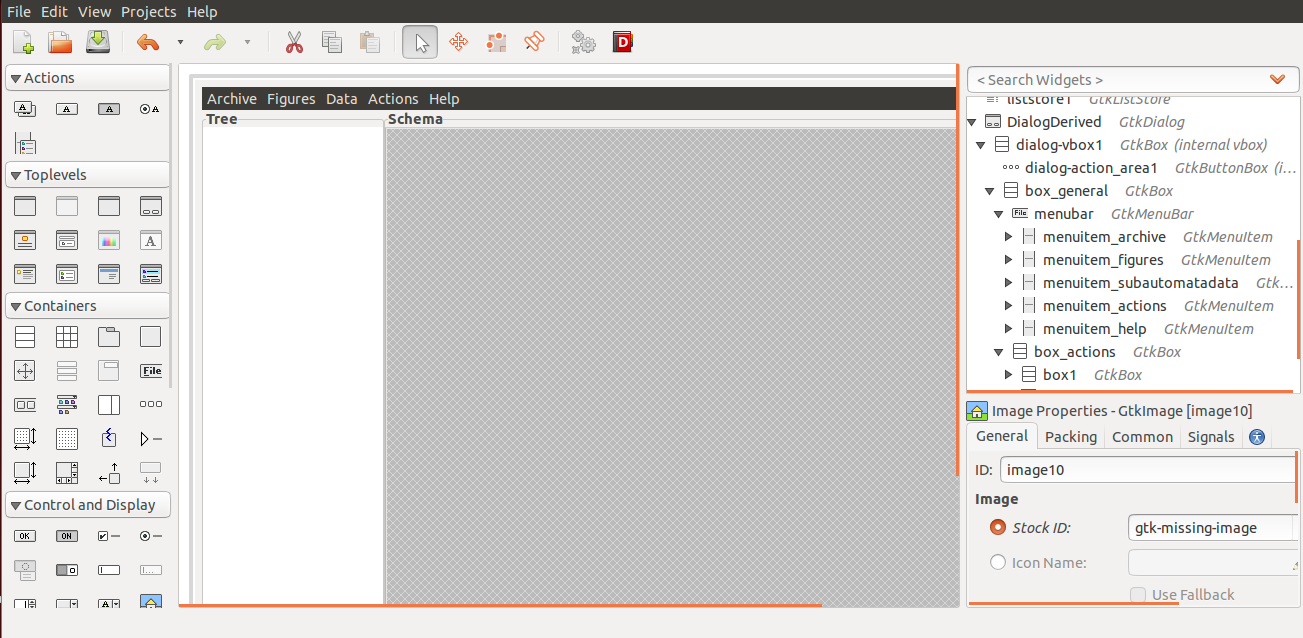
\includegraphics[height=6cm]{imgs/3_infrastructure/gladeEditor.png}
	\caption{Glade Interface Designer.}
	\label{fig:gladeDesigner}
\end{figure}


%%%%%%%%%%%%%%% PyQt4 y PyQt 4 Designer%%%%%%%%%%%%%%%
\section{PyQt4}
%PyQt4
Para el componente en Python, hemos optado por utilizar la versión 4 de PyQt, un \textit{binding} de la biblioteca gráfica Qt, desarrollada por Riverbank Computing\footnote{\url{https://riverbankcomputing.com/}} y disponible para Windows, GNU/Linux y Mac OS X bajo diferentes licencias. Este cambio de librería gráfica se debe principalmente a que al trabajar ahora con aplicaciones en Python, la reutilización del código del editor original, escrito en C++, ya no resulta importante. \\

Qt\footnote{\url{http://www.qt.io/}} es una biblioteca multiplataforma ampliamente utilizada para desarrollar aplicaciones con GUI, desarrollada como un software libre y de código abierto a través de Qt Project, donde participa tanto la comunidad, como desarrolladores de Nokia y Digia, entre otras empresas. Está hecho en C++, pero adicionalmente puede ser utilizado en otros lenguajes de programación mediante \textit{bindings}, estando disponible para Python, C\#, Ruby y Java, entre otros. \\

PyQt4 se encuentra dividido en una serie de componentes que pueden ser importados individualmente como módulos de Python, de los cuales hemos utilizado:

\begin{itemize}
\item \textbf{QtCore:} Contiene las clases que no están directamente relacionadas con la GUI, incluyendo el bucle principal de la interfaz y funciones para trabajar con señales y \textit{slots}.
\item \textbf{QtGui:} Módulo que contiene la mayoría de las clases relacionadas con la GUI.
\end{itemize}

En cuanto al flujo de ejecución, PyQt4 funciona igual que GTK+, quedándose a la espera de que se produzca un evento, y pasándole el control a su manejador cuando este tiene lugar, cómo ya hemos explicado. \\

% Qt 4 Designer
Para diseñar la GUI en tiempo de ejecución con PyQt4 hemos utilizado la herramienta \emph{Qt 4 Designer}, que puede observarse en las figura \ref{fig:qtDesigner}. Al igual que \textit{Glade}, permite realizar el desarrollo de la GUI de forma gráfica guardando el diseño en un archivo XML y permitiendo su carga dinámica en tiempo de ejecución. Sin embargo, nos hemos aprovechado de una de las herramientas que ofrece PyQt4: \textit{pyuic4}. Este programa convierte el archivo XML que se ha diseñado en código Python, de forma que puede importarse como un módulo más, evitando que esta traducción tenga lugar en tiempo de ejecución y minimizando así el tiempo de carga de la GUI. \\

\begin{figure}[htbp]
	\centering
	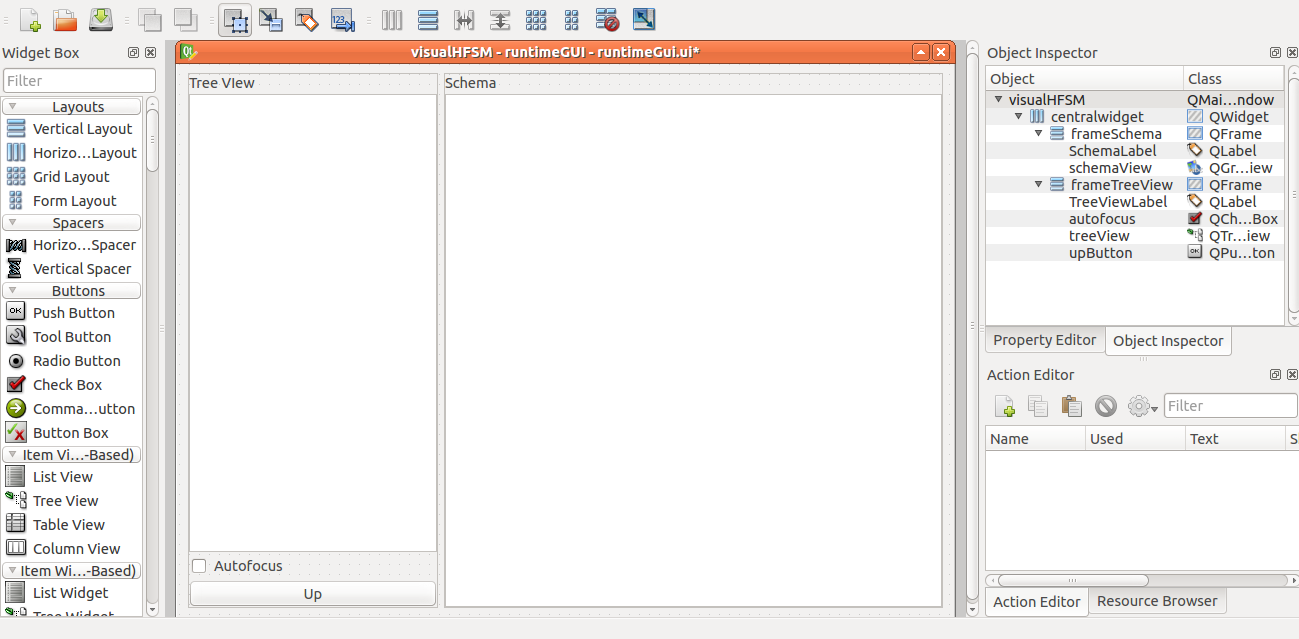
\includegraphics[height=6cm]{imgs/3_infrastructure/qtDesigner.png}
	\caption{Qt 4 Designer.}
	\label{fig:qtDesigner}
\end{figure}
\chapter{VisualHFSM 5.0}\label{chap:VisualHFSM5}
En este capítulo empezaremos comentando brevemente las características principales de la herramienta para poner en situación al lector. Después, describiremos la solución que hemos desarrollado para cumplir los objetivos y los requisitos previamente comentados. La idea es explicar en detalle todas las novedades que introduce VisualHFSM 5.0 y cómo se han llevado a cabo, terminando con las limitaciones que existían en su anterior versión. Para esto, hemos agrupado los cambios en distintas secciones. Primero, empezaremos comentando los cambios relacionados con el propio editor gráfico. Después comentaremos la GUI en ejecución para el componente de C++, para a continuación, hablar sobre la posibilidad de generar código en Python y la GUI en ejecución para estos componentes en Python, que aunque en apariencia es igual se ha realizado de forma distinta, utilizando otra librería gráfica. Por último, hablaremos de las medidas que hemos tomado para dar a conocer nuestra herramienta y facilitar que sea utilizada por terceros. \\

VisualHFSM cuenta con distintas partes bien diferenciadas, como se observa en la figura \ref{fig:partesVisualHFSM}. En primer lugar tiene el \emph{editor gráfico}, que permite crear el diagrama de estados y editar el comportamiento del robot. Todo el comportamiento generado con el editor se guarda en un \emph{archivo XML}, que se utiliza para poder retomar el proyecto más tarde. Además, cuenta con un \emph{generador de código}, que utiliza el archivo XML guardado mediante el editor gráfico y una \emph{plantilla} para generar el código del componente, el archivo de configuración de ICE y el archivo para la compilación de la aplicación, en caso de que sea necesario. En las aplicaciones en C++ el componente se genera al compilar el código fuente, que puede realizarse desde el editor gráfico también, y en las aplicaciones en Python el propio código se genera como un ejecutable, siendo el componente también. 

\begin{figure}[htbp]
	\centering
	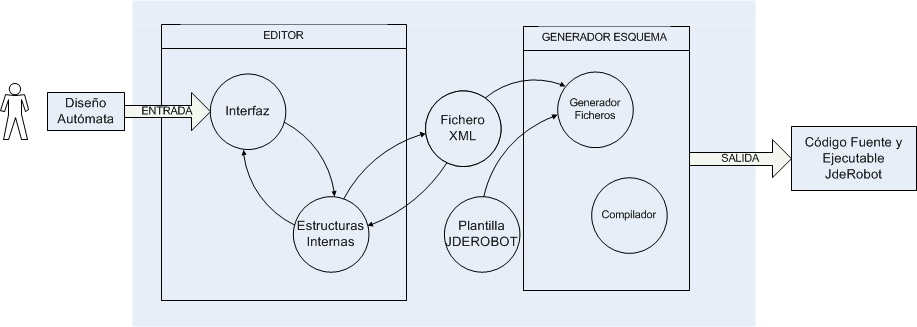
\includegraphics[height=5cm]{imgs/4_visualHFSM5/cajaBlanca.jpg}
	\caption{Esquema con los elementos de VisualHFSM}
	\label{fig:partesVisualHFSM}
\end{figure}


%%%%%%%%%% Mejoras en el editor gráfico %%%%%%%%
\section{Mejoras en el editor gráfico y de usabilidad}
El editor gráfico es el núcleo de VisualHFSM. Es la parte de la herramienta que permite al usuario crear el comportamiento de su autómata de una forma visual mediante un conjunto de estados y transiciones, con posibilidad de añadirles jerarquía. Para conseguir esto, tal y como se observa en la figura \ref{fig:editorVisualHFSM}, el editor de visualHFSM se encuentra dividido en tres partes:

\begin{enumerate}
\item \textit{Schema View:} Se sitúa en la parte de la derecha y es la sección que ocupa la mayor parte del espacio de la GUI. Es el \emph{canvas} en el que se dibujan los estados y transiciones que van a modelar el comportamiento del robot, permitiendo al desarrollador editarlos e interaccionar con ellos. En esta ventana sólo se encuentra representado el \textit{subautómata actual}, por lo que no permite ver toda la jerarquía.
\item \textit{Tree View:} Situado en la parte izquierda de la GUI, muestra la representación textual de todos los estados del autómata que se está editando, agrupados por subautómatas. La jerarquía se indica mediante tabulación. Por ejemplo, en la figura \ref{fig:editorVisualHFSM}, los estados \textit{FindRoad} y \textit{FollowingRoad} pertenecen a un subautómata hijo del estado \textit{FollowRoad}, y por lo tanto aparecen debajo de dicho estado y justificados. Además, los niveles de la jerarquía pueden colapsarse o expandirse a voluntad. Esta vista no permite editar ni interactuar con los estados, pero ofrece una visión global de todo el proyecto, complementando al \textit{Schema View}.
\item \textit{Menú:} Esta sección se sitúa en una barra horizontal en la parte superior y contiene funcionalidad adicional ocupando poco espacio, optimizando el espacio disponible para trabajar con nuestro autómata.
\end{enumerate}

\begin{figure}[htbp]
	\centering
	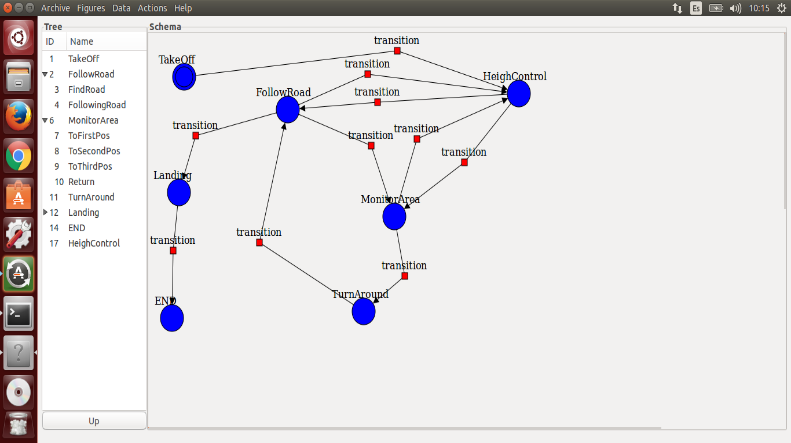
\includegraphics[height=7cm]{imgs/4_visualHFSM5/editor.png}
	\caption{Editor gráfico de VisualHFSM 5.0.}
	\label{fig:editorVisualHFSM}
\end{figure}

Visualmente, el editor gráfico se mantiene igual que en la anterior versión. Sin embargo, aunque no ha habido cambios enormes en la apariencia de la GUI, sí se han realizado distintas modificaciones para mejorar su usabilidad, y se han corregido varios errores del editor que impedían su correcto funcionamiento. \\

%%% Mejora en la navegación por la jerarquía
La modificación principal que hemos realizado al editor gráfico es una mejora de la navegación entre distintos niveles de la jerarquía, de forma que resulte mucho más sencillo cambiar el subautómata seleccionado. Para esto hemos implementado una forma sencilla de navegar hacia los niveles superiores de la jerarquía y una forma rápida de acceder a cualquier subautómata empleando el \textit{Tree View}. \\

Con las versiones anteriores, la forma de visitar el subautómata hijo de un estado era haciendo doble click en dicho estado, pero luego no había forma de volver al subautómata que contenía al estado padre. Para arreglar esto hemos añadido el botón \textit{Up}, que puede verse en la figura \ref{fig:editorVisualHFSM} justo debajo del \textit{Tree View}. Cuando se pulse este botón, los estados y transiciones que se están visualizando en el \textit{Schema View} se ocultan, se busca el subautómata que contiene al estado padre del subautómata actual, y se representan sus estados y transiciones, permitiendo de esta forma volver al nivel superior de la jerarquía. En caso de estar en el subautómata \textit{raíz}, que no tiene ningún padre, el editor simplemente pondrá un mensaje informativo en el terminal indicando que estamos en el subautómata raíz. \\

Además se ha añadido una forma más rápida y sencilla de navegar por los distintos niveles del autómata utilizando el \textit{Tree View}. Para esto, le hemos conectado un manejador a la señal que se emite cuando una fila de nuestro \textit{TreeView} se activa, tal y como se observa en el fragmento de código \ref{lst:connectingSignals}.

\begin{lstlisting}[style=C,caption={conectando un manejador a \texttt{Gtk::TreeView::signal\_row\_activated()}.},label={lst:connectingSignals}]
this->treeview->signal_row_activated().connect(
                 sigc::mem_fun(*this, &VisualHFSM::on_row_activated));
\end{lstlisting}

De esta forma, cada vez que se hace doble click en una fila del \textit{Tree View}, se llama al método \textit{on\_row\_activated}, que puede verse en el fragmento de código \ref{lst:onRowActivated}. Esta función consigue acceder a la fila en la que hemos hecho doble click, y mediante el nombre del estado encuentra el subautómata que lo contiene y lo muestra. De esta forma, se consigue una navegación más dinámica y natural a través de los distintos niveles de la jerarquía. \\

\begin{lstlisting}[style=C,caption={función \texttt{on\_row\_activated}.},label={lst:onRowActivated}]
void VisualHFSM::on_row_activated(const Gtk::TreeModel::Path& path,
                                    Gtk::TreeViewColumn* /* column */){
    Gtk::TreeModel::iterator iter = this->refTreeModel->get_iter(path);

    if (iter){
        Gtk::TreeModel::Row row = *iter;

        std::stringstream name;
        name << row[m_Columns.m_col_name];
        GuiSubautomata* gsub = this->getSubautomataByNodeName(name.str());

        if (gsub == NULL)
            return;

        if (gsub->getId() != this->currentSubautomata->getId()){
            this->currentSubautomata->hideAll();
            this->currentSubautomata = gsub;
            this->currentSubautomata->showAll();
        }
    }else{
        std::cerr << "Couldn't get the row" << std::endl;
    }
}
\end{lstlisting}

%%% Función shutDown() %%%
También hemos añadido la función \textit{shutDown()}, que nos permite finalizar la ejecución del autómata cuando la invocamos. Esto resuelve otra limitación que existía en las versiones anteriores de VisualHFSM, en la que los autómatas nunca terminaban su ejecución, si no que era necesario detener el proceso desde el terminal. Este comportamiento se debe a que los subautómatas se encuentran ejecutándose en un bucle infinito, tal como mostramos en el código a continuación (fragmento de código \ref{lst:loop}).

\begin{lstlisting}[style=C,caption={Ejemplo de un bucle infinito dentro del hilo de un subautómata.},label={lst:loop}]
void* subautomata_1 ( void* ) {
	//variable declaration
	.....

	while (true) {
		gettimeofday(&a, NULL);
		totala = a.tv_sec * 1000000 + a.tv_usec;

		// Evaluation switch
		......

		// Actuation switch
		.....

		//Frecuency Loop Control
		.... 
	}
}
\end{lstlisting}

Aunque esto podría resultar conveniente en algunos casos, definitivamente no lo es siempre, por lo que ahora cuando el generador de código escribe nuestro componente, le añade un \textit{built-in}, la función \textit{shutDown}, que provoca el fin de la ejecución. Para esto, hemos sustituido el \textit{true} de nuestro bucle while por una serie de variables, inicializadas a \textit{true}, de forma que cuando llamamos a la función \textit{shutDown}, cambiará el valor de estas variables a \textit{false}, rompiéndose así el bucle infinito y permitiendo que el código alcance el final sin necesidad de interrumpirlo externamente mediante la consola. \\


%%% Mejora archivo .cfg %%%
Con esta versión de VisualHFSM también hemos mejorado la creación de los archivos de configuración, dotándolos de mayor flexibilidad, de forma que la herramienta es compatible con cualquier robot, real o simulado, cuyas interfaces estén disponibles dentro de la plataforma JdeRobot. Para esto, hemos incluido el campo \textit{Proxy Name}, que permite al usuario elegir este parámetro, como puede observarse en la figura \ref{fig:cfgFileGeneration}. Esto supone una ventaja dado que anteriormente este nombre dependía de la interfaz que se utilizaba. Sin embargo, distintas aplicaciones pueden utilizar diferentes nombres para crear el proxy de una misma interfaz. Esto sucede por ejemplo al utilizar el simulador Gazebo, donde para conectarse a la cámara el \textit{proxy} se llamaba \emph{Camera}, mientras que al utilizar la aplicación \textit{ardrone\_server} para conectarnos al robot real, el nombre que éste recibe es \emph{ardrone\_camera}. Esta modificación permite solventar estas situaciones, haciendo la herramienta completamente compatible con robots simulados y reales, mientras que en las versiones anteriores sería necesario modificar manualmente el archivo de configuración generado para que el componente desarrollado funcionase.

\begin{figure}[htbp]
	\centering
	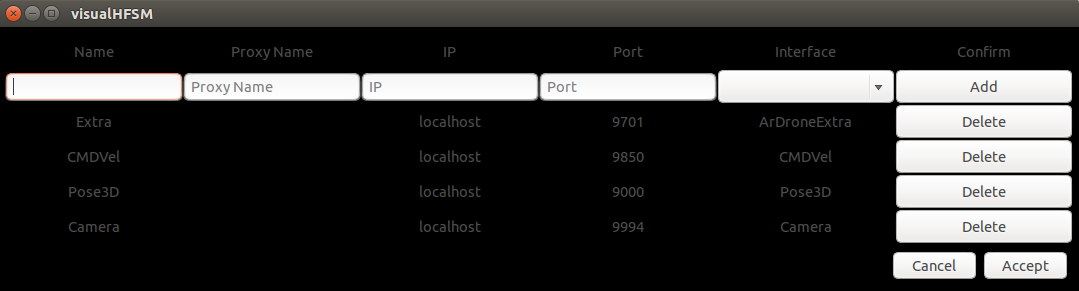
\includegraphics[height=4cm]{imgs/4_visualHFSM5/configFiles.png}
	\caption{Formulario para editar el archivo de configuración.}
	\label{fig:cfgFileGeneration}
\end{figure}


%%% Dependencias resueltas
Otra mejora añadida ha sido resolver las dependencias de la herramienta para permitir ejecutarla desde cualquier directorio. Esta era otra limitación presente en VisualHFSM, dado que sólo podía abrirse desde la carpeta visualHFSM donde estaba todo su código. Esto suponía un problema especialmente porque con la última versión de JdeRobot la instalación puede realizarse mediante paquetes debian sin necesidad de descargarte el código, por lo que para poder utilizar visualHFSM era necesario descargarte el código a parte de GitHub\footnote{\url{https://github.com/RoboticsURJC/JdeRobot/tree/master/src/stable/tools/visualHFSM}}, y compilarlo siguiendo las instrucciones del manual\footnote{\url{http://jderobot.org/index.php/Manual-5\#Installing_JdeRobot_5}}. La razón de que sólo pudiese ejecutarse desde su propia carpeta es que para ejecutar el editor gráfico, necesitaba cargar los distintos archivos \textit{.glade}, tanto del editor como de sus \textit{popups}.  \\

Para solucionar este problema, hemos creado un script para su instalación, \textit{setup.sh}, que aprovechándose de los directorios creados por JdeRobot durante su instalación, copia todos los archivos \textit{.glade} en el directorio \textit{/usr/local/share/jderobot/glade/visualHFSM/}, para los componentes en C++, en \textit{/usr/local/share/jderobot/python/visualHFSM\_py} para los componentes en Python, y en \textit{/usr/local/bin} para el script \textit{getinterfaces.sh}. Con esta nueva distribución, y al cambiar los \textit{paths} de carga de los distintos archivos, conseguimos que el ejecutable de visualHFSM (también situado en \textit{/usr/local/bin}), pueda ejecutarse desde cualquier directorio, dado que sus dependencias estarán instaladas siempre en unas direcciones por defecto. \\


%%% Bug abrir nuevos proyectos
Uno de los errores más molestos que se han solucionado está relacionado con abrir nuevos proyectos cuando estábamos trabajando con otro. El problema era que, al estar trabajando con un proyecto, y abrir otro, el \textit{Tree View} no se limpiaba, sino que pasaba a tener los estados del antiguo proyecto, y del nuevo. Esto, además de ser molesto, creaba problemas en la navegación entre niveles de la jerarquía, dado que aparecían IDs repetidos, que se correspondían a estados no existentes en el proyecto, pero sí en el \textit{Tree View}, lo que podía originar errores al programa. \\


%%% Bug IDs
Por último, otro de los fallos que se han solucionado podía ocasionar que un proyecto quedase inservible, y estaba también relacionado con los IDs. A la hora de crear nuevos estados, transiciones o subautómatas, se les asignaba un ID que debía ser único, que permitía identificarlos. Estos IDs se generaban a partir de 3 variables, como vemos en el código \ref{lst:ids}.

\begin{lstlisting}[style=C,caption={Variables utilizadas para generar los distintos ids.},label={lst:ids}]
class VisualHFSM : public Gtk::Dialog {
	.......
private:
    int id;			// ID for the subautomata created
    idguinode;		// ID for the state created
    idguitransition;// ID for the transition created
    ....
}
\end{lstlisting}

Y dichas variables se incrementaban en uno cuando se creaba un subautómata, estado o transición, respectivamente. El problema aparecía en que, al borrar un estado o subautómata, sus ID también se reducían en uno, pudiendo aparecer así identificadores repetidos que, nuevamente, ocasionaban que la herramienta no funcionase de manera adecuada.


%%%%%%%%%% GUI en ejecución para C++ %%%%%%%%%%
\section{GUI en ejecución para C++}
Como ya hemos comentado en capítulos anteriores, la GUI en ejecución es una característica que visualHFSM tenía en sus primeras versiones y que perdió al dar soporte a autómatas jerárquicos. Esta característica consiste en una GUI de aspecto muy similar a la del editor gráfico, que muestra dinámicamente qué estados están activos durante la ejecución del componente generado por VisualHFSM 5.0. Ésto resulta muy deseable, dado que ahorra mucho tiempo en la depuración al permitir comprobar si el autómata se está comportando como esperamos que haga en tiempo de ejecución, y, en caso de no hacerlo, ver qué es lo que ha pasado y por qué ha podido tener lugar este fallo. La recuperación de esta característica fue el motivo inicial de este TFG.  \\

%%% Explicación general
Para la GUI en ejecución hemos creado la clase \textit{AutomataGui}, que se ejecutará como una aplicación GTK de la clase \textit{Gtk::Application}. Esta clase se importa en el componente creado, se inicializa un objeto, se carga el \textit{glade} y el autómata, y en caso de que todo haya ido bien se ejecutará la GUI en tiempo de ejecución. Si hubiese algún problema durante estos pasos, se notificaría mediante un mensaje en la terminal, pero la ejecución del robot continuaría como si nada hubiese pasado, sin perjudicarle el hecho de que la GUI haya fallado. \\

%%% Como arrancar la GUI
Aunque esta característica es muy conveniente, sólo tiene sentido para depurar, por lo que por defecto el componente se ejecutará sin ella. Esto se debe a que, cuando sepamos que el código funciona como esperamos, y lo ejecutemos en un robot, puede que no estemos interesados en gastar recursos creando un hilo adicional para mostrar la GUI. Por lo tanto, si queremos ejecutar el componente con ella, deberá lanzarse con el argumento \textit{--displaygui=true}, tal como se ve en el ejemplo \ref{lst:executingWithGUI}

\begin{lstlisting}[style=C,caption={Comando para ejecutar un componente C++ con GUI en ejecución.},label={lst:executingWithGUI}]
	monitorArea --Ice.Config=monitorArea.cfg --displaygui=true
\end{lstlisting}

%%% Inicialización
Por lo tanto, al arrancar el componente generado con nuestra herramienta de la forma que acabamos de ver, en primer lugar se leerán los argumentos, y, al encontrar el argumento \textit{--displaygui=true} se pondrá a \textit{true} la variable \textit{displayGui}. A continuación, se conectará a las interfaces ICE que sean necesarias, y después, como \textit{displayGui} es verdad, crea un objeto de la clase \textit{AutomataGui}, pasándole como argumentos los argumentos con los que hemos lanzado el componente, y se llamará a la función \textit{showAutomataGui()}. Esta función se encarga de inicializar el objeto, crear la lista de subautómatas necesaria para su representación gráfica, y si todo ha ido bien, crear un nuevo hilo en el que se ejecutará la aplicación GTK. Esto puede verse en el fragmento de código \ref{lst:initAutomataGui}. \\

\begin{lstlisting}[style=C,caption={Código encargado de inicializar el objeto automatagui.},label={lst:initAutomataGui}]
bool showAutomataGui () {
	if (automatagui->init() < 0){
		std::cerr << "warning: could not show automatagui" << std::endl;
		return false;
	}
	automatagui->setGuiSubautomataList(createGuiSubAutomataList());
	pthread_create(&thr_automatagui, NULL, &runAutomatagui, NULL);
	automatagui->loadGuiSubautomata();
	return true;
}

int main (int argc, char* argv[]) {
	int status;
	Ice::CommunicatorPtr ic;

	try {
		ic = Ice::initialize(argc, argv);
		readArgs(&argc, argv);

		// Create proxys
		.....
		
		if (displayGui){
			automatagui = new AutomataGui(argc, argv);
			displayGui = showAutomataGui();
		}

		//create subautomatas threads
		pthread_create(&thr_sub_1, NULL,
		 &subautomata_1, NULL);

		//join subautomatas threads
		pthread_join(thr_sub_1, NULL);
		if (displayGui)
			pthread_join(thr_automatagui, NULL);
			
	} catch ( const Ice::Exception& ex ) {
		std::cerr << ex << std::endl;
		status = 1;
	} catch ( const char* msg ) {
		std::cerr << msg << std::endl;
		status = 1;
	}

	if (ic)
		ic->destroy();

	return status;
}
\end{lstlisting}

La inicialización se encarga de cargar el archivo \textit{.glade} que contiene la GUI, y de inicializar algunos de sus componentes gráficos como el \textit{Tree View} o el botón \textit{Up}, y de asignar los manejadores a las señales necesarias para poder responder de manera adecuada a los eventos que sucedan en la GUI. \\

Una vez que hemos inicializado nuestro objeto, es necesario crear la lista de subautómatas, con los nodos y transiciones que contiene cada uno para poder representarlos. Aquí nos enfrentamos a un primer problema, dado que, para construir esta lista en el editor gráfico es necesario analizar el archivo XML con el que se está trabajando, pero esto haría que los componentes generados dependiesen del fichero XML, que puede estar en cualquier sitio. Para solucionar esto, nos hemos aprovechado de que el generador de código ya tiene acceso a esta lista de subautómatas, por lo que al generar el componente, le escribe la función \textit{createGuiSubAutomataList()}, de forma que al ejecutarla va creando los subautómatas correspondientes, y les va añadiendo sus estados y transiciones, con las coordenadas en las que deberán pintarse. Para esto, el generador de código se recorre las listas de estados y transiciones de cada subautómata, de forma que sabe qué parámetros tiene que pasarle a los constructores para acabar teniendo la misma lista. Un ejemplo de esta función puede verse en el código de ejemplo \ref{lst:createGuiSubAutomataList}.

\begin{lstlisting}[style=C,caption={Función createGuiSubAutomataList() creada por el generador de código.},label={lst:createGuiSubAutomataList}]
std::list<GuiSubautomata> createGuiSubAutomataList(){
	std::list<GuiSubautomata> guiSubautomataList;
	//Creating the subautomata
	GuiSubautomata* guiSubautomata1 = new GuiSubautomata(1, 0);

	//Creating and adding nodes to this subautomata
	guiSubautomata1->newGuiNode(1, 0, 163, 201);
	guiSubautomata1->setIsInitialLastGuiNode(1);
	guiSubautomata1->setNameLastGuiNode("GO");

	guiSubautomata1->newGuiNode(2, 0, 539, 238);
	guiSubautomata1->setIsInitialLastGuiNode(0);
	guiSubautomata1->setNameLastGuiNode("wait");

	//Creating and adding nodes to this subautomata
	Point* origin11 = new Point(163, 201);
	Point* destiny11 = new Point(539, 238);
	Point* midPoint11 = new Point(357, 116);
	guiSubautomata1->newGuiTransition(*origin11,
					 *destiny11, *midPoint11, 1, 1, 2);

	Point* origin12 = new Point(539, 238);
	Point* destiny12 = new Point(163, 201);
	Point* midPoint12 = new Point(342, 308);
	guiSubautomata1->newGuiTransition(*origin12,
					 *destiny12, *midPoint12, 2, 2, 1);

	guiSubautomataList.push_back(*guiSubautomata1);

	return guiSubautomataList;
}
\end{lstlisting}

%%% Comparación GUIs
Una vez que el objeto \textit{automatagui} ha sido correctamente inicializado, la interfaz gráfica se mostrará en pantalla, tal y como se muestra en la figura \ref{fig:newRuntimeGuiCPP}, donde podemos ver que los estados activos se pintan en verde, tanto en el \textit{Schema View} como en el \textit{Tree View}, en los distintos niveles de la jerarquía. \\
 
\begin{figure}[htbp]
	\centering
	\begin{subfigure}{0.45\textwidth}
	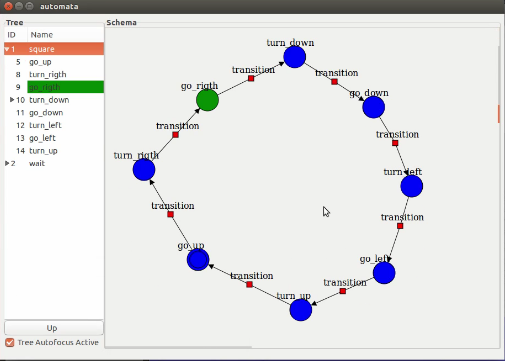
\includegraphics[height=5cm]{imgs/4_visualHFSM5/newRuntimeGuiCPP.png}
	\caption{Nueva GUI en tiempo de ejecución.}
	\label{fig:newRuntimeGuiCPP}
	\end{subfigure}
	\hfill
	\centering
	\begin{subfigure}{0.45\textwidth}
	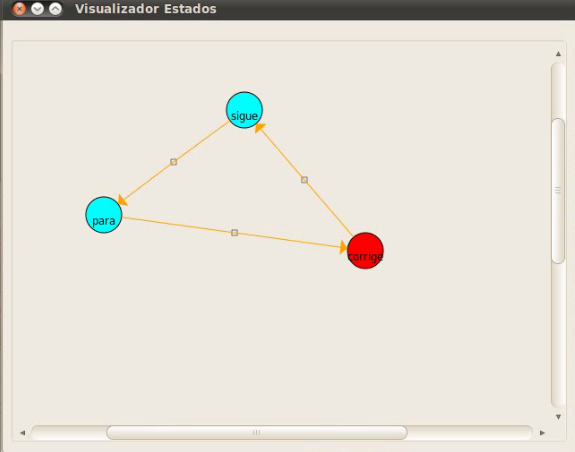
\includegraphics[height=5cm]{imgs/4_visualHFSM5/oldRuntimeGui.png}
	\caption{Antigua GUI en tiempo de ejecución.}
	\label{fig:oldRuntimeGui}
	\end{subfigure}
\caption{Comparación de la nueva y la antigua GUI en tiempo de ejecución.}
\label{oldVsNew}
\end{figure}


Al cargar la GUI por primera vez, cuando se crea un estado se comprueba si es un estado activo. Para esto, tiene que ser el estado inicial de su subautómata, y todos sus padres (en caso de tenerlos), también deben ser el estado inicial. Si esto se cumple, este estado se pintará de verde en el \textit{Schema View} y con el fondo en este mismo color en el \textit{Tree View}. En caso contrario, el estado se pintará de azul en el \textit{Schema View} y se dejará el fondo blanco en el \textit{Tree View}. Con esto se consigue que los primeros nodos activos se representen en la GUI como queremos.  \\

El siguiente paso es que cuando se produce una transición entre estados, se cambien los colores en la GUI para actualizar la representación, pero si la GUI se ejecuta desde un hilo que no sea el principal puede dar problemas y terminar su ejecución. Para arreglar esto, hemos utilizado un objeto \textit{Glib::Dispatcher dispatcher} y la función \textit{notifySetNodeAsActive(std::string nodeName)}. Cuando en un subautómata tiene lugar una transición, en su hilo se llama a esta función con el nombre del nodo que hay que marcar como activo. Esta función introduce el nombre en una cola síncrona, para evitar problemas de condiciones de carrera, y hace que el objeto \textit{dispatcher} emita una señal, que será recogida por un manejador en el hilo de la GUI. Cuando el manejador se activa, extrae el primer nombre que se ha introducido en la cola y busca el subautómata que lo contiene. Entonces, marca como no activado al anterior nodo activo y activa el nuevo estado. En el fragmento de código \ref{lst:notifySetActive} se puede ver el código que se encarga del proceso descrito.

\begin{lstlisting}[style=C,caption={Ejemplo de como se notifica a la GUI que debe cambiar el nodo activo.},label={lst:notifySetActive}]
void AutomataGui::on_notify_received(){

	pthread_mutex_lock(&this->activesNodesNames.lock);
	if (this->activesNodesNames.queue.empty()){
		std::cerr << "ERROR: actives nodes names queue is empty" << std::endl;
		return;
	}
	std::string activeName = this->activesNodesNames.queue.front();
	this->activesNodesNames.queue.pop();
	pthread_mutex_unlock(&this->activesNodesNames.lock);

	GuiSubautomata* subautomata = this->getSubautomataByNodeName(activeName);
	std::string lastActive = subautomata->getActiveNode();
	GuiNode* node;

	node = subautomata->getGuiNode(lastActive);
	this->setNodeAsActive(node, subautomata, false);

	node = subautomata->getGuiNode(activeName);
	this->setNodeAsActive(node, subautomata, true);
}


void AutomataGui::notifySetNodeAsActive(std::string nodeName){
	pthread_mutex_lock(&this->activesNodesNames.lock);
	this->activesNodesNames.queue.push(nodeName);
	pthread_mutex_unlock(&this->activesNodesNames.lock);
	this->dispatcher.emit();
}
\end{lstlisting}

Además, en el fragmento de código \ref{lst:setNodeAsActive} se observa que la función \textit{setNodeAsActive} actualiza el estado el nodo que recibe como argumento, y comprueba si tiene algún hijo, y en caso de tenerlo se llama concurrentemente a sí misma pero pasándole como nodo el nombre de su nodo hijo. De esta forma, se actualiza el estado del nodo y de todos sus hijos.

\begin{lstlisting}[style=C,caption={función setNodeAsActive},label={lst:setNodeAsActive}]
void AutomataGui::setNodeAsActive(GuiNode* node,
								 GuiSubautomata* subautomata, bool active){
	if(active){
		subautomata->setActiveNode(node->getName());
		node->changeColor(ITEM_COLOR_GREEN);
	}else{
		node->changeColor(ITEM_COLOR_BLUE);
	}

	if(!this->setActiveTreeView(node->getName(), 
		active, this->refTreeModel->children()))
 		std::cerr << "NOT FINDED " << node->getName() << std::endl;	

 	int sonId = node->getIdSubautomataSon();
 	if (sonId != 0){
 		GuiSubautomata* subSon = this->getSubautomata(sonId);
 		std::string nodeName = subSon->getActiveNode();
 		GuiNode* nodeAux = subSon->getGuiNode(nodeName);
 		this->setNodeAsActive(nodeAux, subSon, active);
 	}
}
\end{lstlisting}

Por último, en la figura \ref{oldVsNew} podemos ver una comparación de la nueva y la vieja GUI en ejecución. Como se puede observar son completamente distintas, dado que hemos optado por que la apariencia de esta GUI sea lo más similar posible a la del editor gráfico. Además, se le ha añadido el \textit{Tree View}, que permite ver el estado general del autómata, monitorizando que todos los estados activos en toda la jerarquía, no sólo en el nivel actual. \\

%%%%% EJEMPLOS DE VALIDACIÓN
Todas las funcionalidades descritas en este apartado han sido validadas experimentalmente. Para mostrar esto, hemos seleccionado una de las varias aplicaciones que hemos desarrollado utilizando componentes en C++, la aplicación \textit{Cuadrado con un Pioneer}, que será explicada en detalle en el capítulo 5.


%%%%%%%%%% Generación de código Python %%%%%%%%%%
\section{Generación de código en Python}
Otra de las grandes mejoras que tiene VisualHFSM 5.0 frente a otras versiones es que se ha ampliado el generador de código automático de forma que ahora permite generar código en Python también. Esto aumenta en gran medida la flexibilidad y potencia de la herramienta, dado que ahora ofrece soporte para los dos lenguajes, y además, se acerca más a la tendencia de los componentes de JdeRobot, donde los programas en Python son cada vez más habituales. Python es un lenguaje elegante, cómodo y flexible que está teniendo una gran acogida en el mundo de la robótica, que resulta especialmente interesante por los siguientes motivos:

\begin{itemize}
\item Se trata de un lenguaje interpretado, no compilado. Esto resulta increíblemente práctico, y además, en nuestra herramienta ahorra la necesidad de generar un fichero CMake para realizar la compilación, que además tarda algunos minutos. Resulta muy cómodo realizar cambios y probarlos directamente sin necesidad de compilar.
\item Su sintaxis es especialmente clara y directa, lo que hace que sea un lenguaje muy fácilmente legible.
\item Su tiempo de ejecución de sus instrucciones está muy cercano al de programas escritos en C, algo muy importante para la robótica.
\item La gestión de la memoria se hace de forma automática. No resulta necesario la declaración de variables ni liberar espacio.
\item Ofrece tipos de datos de alto nivel como \textit{strings}, tuplas, listas, diccionarios o archivos, entre otros, con una gran variedad de funciones para trabajar con ellos de forma cómoda.
\item Tiene una enorme librería estándar, lo cual añade un gran grado de libertad a la hora de trabajar con este lenguaje.
\end{itemize}

Para generar el código en Python, se ha creado una nueva plantilla donde se empotrará el código de los estados y las transiciones introducido por el desarrollador mediante el editor gráfico, así como el resto de variables y funciones auxiliares que pueda considerar necesarias. Se trata de una plantilla multihilo, en la que se crea un hilo distinto por cada subautómata. Al compararla con la plantilla en C++, se trata de una plantilla mejor organizada, con menos posibilidades de fallos inesperados y un código final más legible. Además, el archivo \textit{.py} generado se creará como un ejecutable, de forma que puede utilizarse del mismo modo que se utilizaban los componentes de C++. \\

La plantilla que se utiliza para generar el código en Python no es la misma que la que se utilizaba en C++, si no que ahora sigue un modelo de programación orientada a objetos, donde todos los datos y funciones del autómata se encuentran dentro de la clase \textit{Autómata}, de forma que la comunicación entre distintos subautómatas es mucho más sencilla, dado que es posible la utilización de elementos de la clase para ello. Además, al usar una plantilla basada en la programación a objetos, conseguimos también la posibilidad de crear clases internas, de forma que el desarrollador cuenta con más herramientas para organizar el código como mejor le parezca, pero manteniendo un alto nivel de abstracción.  \\

Por último, el componente en Python cuenta también con un objeto \textit{threading.Lock()}, por si el código que se va a ejecutar es sensible a las condiciones de carrera. Hay que tener en cuenta para esto que, cada subautómata sigue ejecutándose como un hilo distinto cada uno, por lo que es muy probable que aparezcan condiciones de carrera si se utilizan distintos niveles de jerarquía dentro del autómata. \\

\begin{figure}[htbp]
	\centering
	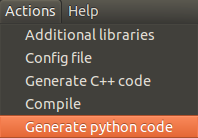
\includegraphics[height=3cm]{imgs/4_visualHFSM5/generatePythonCode.png}
	\caption{Menú con la opción de generar codigo Python.}
	\label{fig:pythonCodeGenerator}
\end{figure}


%EXPLICACION SENCILLA DEL LA PLANTILLA
Al generar el código la plantilla se va completando dinámicamente en función a la información introducida con el editor gráfico. En resumen, para este proceso se generan las cabeceras que importan todas las librerías necesarias, tanto por defecto como las introducidas por el usuario. Entonces, se genera la clase autómata, donde se definen todas las variables y funciones que el usuario haya introducido. Adicionalmente, se generan las funciones de los subautómatas, una por cada subautómata existente. Dichas funciones serán ejecutadas cada una en un hilo distinto y se encargan de revisar si toca transitar a otro estado, y de ejecutar el código correspondiente en caso de ser necesario. Después se crea la función encargada de que los subautómatas comiencen su ejecución, la función encargada de esperar a que terminen, la función responsable de conectarse al robot y la función \texttt{shutDown()}, que terminará la ejecución en caso de que sea llamada. Por último, fuera de la clase autómata, se genera el cuerpo del \texttt{main}, que será llamado cuando ejecutemos el componente generado y se encargará de llamar a las funciones encargadas de conectarse al robot, empezar la ejecución de los distintos subautómatas y quedarse esperando a que estos hilos finalicen. \\


%%% Descripción del generador de código
A continuación abordaremos este proceso en detalle. Cuando el autómata está preparado, al hacer click en el menú \textit{Actions} a la opción de \textit{Generate Python code}, tal y como se ve en la figura \ref{fig:pythonCodeGenerator}, se activa su manejador, la función \textit{on\_menubar\_clicked\_generate\_python\_code}. Esta función se encarga de analizar el último archivo XML guardado del proyecto mediante un objeto \textit{SaxParser}, preparar la cadena con la ruta al archivo XML y prepararlo para generar la ruta para el archivo Python y el archivo de configuración para ICE, y cuando ha terminado con esto, crea un objeto generador de código y llama a la función \texttt{init\_py()}. \\

\begin{lstlisting}[style=python,caption={Función \texttt{init\_py()} del generador de código.},label={lst:initPy}]
int Generate::init\_py (){
	this->fs.open(this->path.c_str(), std::fstream::out);
	if (this->fs.is_open()){
		this->generateHeaders_py();
		this->generateAutomataClass_py();
		this->generateMain_py();
		this->fs.close();

		this->fs.open(this->cfgpath.c_str(), std::fstream::out);
		if (this->fs.is_open()){
			this->generateCfg();
			this->fs.close();
		}

		std::string permission("chmod +x " + this->path);
		system(permission.c_str());
		return 0;
	}else{
		return -1;
	}
}
\end{lstlisting}

Como podemos observar, la función que vemos en el fragmento de código \ref{lst:initPy} es la encargada de escribir todo el código del componente y su archivo de configuración, así como de otorgarle permisos de ejecución. Para esto sigue los siguientes pasos:

\begin{enumerate}
\item Abrir el fichero en el que se va a escribir el código, cuya ruta se le ha pasado al constructor de la clase \textit{Generate} como argumento. A continuación comprueba que el fichero se haya abierto correctamente, devolviendo -1 para notificar que ha habido un error en caso contrario.
\item La función \texttt{generateHeaders\_py} se encarga de escribir \texttt{\#!/usr/bin/python} para que cuando el código sea un ejecutable sea interpretado por el intérprete de Python y se encarga de realizar los \texttt{imports} necesarios. Para esto, importa las librerías adicionales que se le han añadido mediante el editor, las interfaces de JdeRobot que se van a utilizar para conectarse a los sensores y actuadores, y algunas otras librerías necesarias como \texttt{sys}, \texttt{signal} o la clase \texttt{AutomataGui} del módulo \texttt{automatagui}, entre otros.
\item \texttt{generateAutomataClass\_py} se encarga de escribir toda la información relativa al autómata.
\item A continuación la función \texttt{generateMain\_py} se encarga de generar el cuerpo del main. Esto es el código que será ejecutado cuando se ejecute el componente.
\item Tras generar el cuerpo del \texttt{main}, y se abre otro nuevo para escribir el archivo de configuración. De esto se encarga la función \texttt{generateCfg()}, que es la misma que ya existía en el generador de código C++.
\item Por último, cuando todo el código ha sido generado, la función le da permisos de ejecución para que pueda ejecutarse como un script, sin necesidad de llamar al intérprete Python por la línea de comandos.
\end{enumerate}

\begin{lstlisting}[style=python,caption={Función \texttt{generateAutomataClass\_py()}.},label={lst:generateAutomataClass}]
void Generate::generateAutomataClass_py(){
	this->fs << "class Automata():" << std::endl;
	this->fs << std::endl;
	this->generateAutomataInit_py();
	this->generateFunctions_py();
	this->generateStartThreads_py();
	this->generateCreateGuiSubautomataList_py();
	this->generateShutDown_py();
	this->generateRunGui_py();
	this->generateSubautomatas_py();
	this->generateConnectToProxys_py();
	this->generateDestroyIc_py();
	this->generateStart_py();
	this->generateJoin_py();
	this->generateReadArgs_py();
}
\end{lstlisting}

Como se puede deducir de la explicación anterior, la función responsable de generar casi todo el código del autómata es \textit{generateAutomataClass\_py}, la cual puede verse en el código \ref{lst:generateAutomataClass}. Esta función también se basa en otras funciones secundarias para realizar el trabajo de una forma más organizada y legible. En primer lugar, \textit{generateAutomataInit\_py()} se encarga de escribir el constructor, donde se inicializa el \textit{lock} para ese autómata, la variable \textit{self.displayGui} con valor \textit{False} por defecto, los \textit{arrays} con los distintos estados de cada subautómata y las variables donde se guarda el estado actual en el que se encuentra cada autómata así como las variables que controlan si se sigue entrando en el bucle de ejecución. Podemos ver un ejemplo de constructor creada por esta función en \ref{lst:initExample}.

\begin{lstlisting}[style=python,caption={Ejemplo de constructor creado por el generador de código},label={lst:initExample}]

	def __init__(self):
		self.lock = threading.Lock()
		self.displayGui = False
		self.StatesSub1 = [
			"PingPong",
			"Numbers",
		]

		self.StatesSub3 = [
			"Ping",
			"Ping_ghost",
			"Pong",
			"Pong_ghost",
		]

		self.StatesSub4 = [
			"1",
			"1_ghost",
			"2",
			"2_ghost",
			"3",
			"3_ghost",
		]

		self.StatesSub5 = [
			"wait2",
			"wait2_ghost",
			"wait1",
			"wait1_ghost",
		]

		self.sub1 = "Numbers"
		self.run1 = True
		self.sub3 = "Ping_ghost"
		self.run3 = True
		self.sub4 = "1_ghost"
		self.run4 = True
		self.sub5 = "wait1_ghost"
		self.run5 = True
\end{lstlisting}

Una vez que se ha generado la función \texttt{init}, se escriben las funciones que el usuario ha creado mediante el editor gráfico (en caso de haberlas), y la función \textit{startThreads()}, que será llamada para empezar los hilos de los distintos subautómatas. A continuación se escribirá la función \textit{shutDown()}, que funciona igual que en el componente C++, la función que permite generar la lista de subautómatas necesaria para la GUI en tiempo de ejecución. Después se generan las funciones que llamarán los hilos de los subautómatas, con todas sus variables, su \texttt{if} de evaluación y su \texttt{if} de actuación, dado que en Python no existen los \textit{switch}, escribiendo entonces la función que se encargará de comunicarse con los sensores y actuadores usando ICE y la función para eliminar el objeto ICE al terminar la ejecución. Por último se generará la función encargada de iniciar la GUI en tiempo de ejecución, la función que se llamará para esperar a que los hilos terminen y la \textit{readArgs()}, encargada de leer los argumentos de entrada. \\

Para terminar con esta sección, comentaremos cómo es el generador del \texttt{main}, que puede verse en el fragmento de código \ref{lst:mainExample}. En este caso, el \texttt{main} generado es igual para todos los autómatas, dado que lo que varía es el contenido de las funciones que llama. Comparándolo con el \texttt{main} de los componentes de C++ se trata de un \texttt{main} más compacto y legible, dado que toda la funcionalidad ha sido organizada en funciones que se encargan de realizar el trabajo necesario. \\

\begin{lstlisting}[style=python,caption={Función encargada de generar el cuerpo del programa en Python.},label={lst:mainExample}]

void Generate::generateMain_py (){
	this->fs <<
"if __name__ == '__main__':\n\
	signal.signal(signal.SIGINT, signal.SIG_DFL)\n\
	automata = Automata()\n\
	try:\n\
		automata.connectToProxys()\n\
		automata.readArgs()\n";

	this->fs.flush();
	this->fs <<
"		automata.start()\n\
		automata.join()\n\n\
		sys.exit(0)\n\
	except:\n\
		traceback.print_exc()\n\
		automata.destroyIc()\n\
		sys.exit(-1)\n";
}
\end{lstlisting}


%%%%%%%%%% GUI en ejecución para Python %%%%%%%%
\section{GUI en ejecución para Python}
Al igual que sucede con los componentes generados en C++, los componentes escritos en Python también disponen de una GUI en tiempo de ejecución para depurar. En este caso no se ha utilizado GTK, si no que en su lugar se ha optado por realizarla utilizando Qt, a través de su \textit{binding} para Python: \textit{PyQt}, en su versión 4, tal y cómo explicamos en el capítulo 3 de esta memoria.

\begin{figure}[htbp]
	\centering
	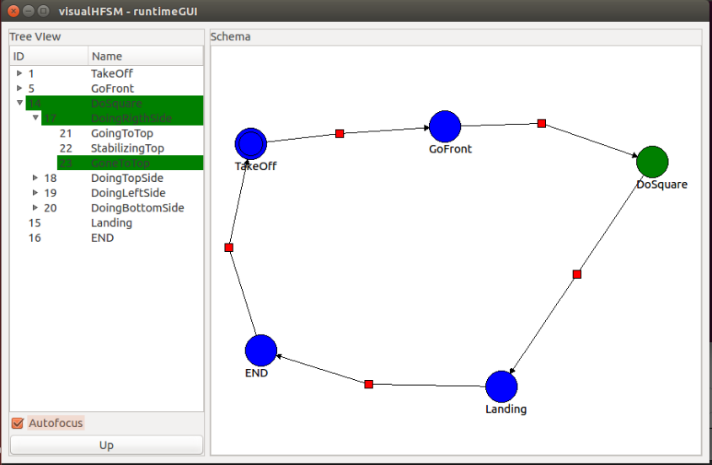
\includegraphics[height=5cm]{imgs/4_visualHFSM5/runtime.png}
	\caption{GUI en tiempo de ejecución con "Autofocus" activo.}
	\label{fig:runtimeGUIPython}
\end{figure}

Sin embargo, a pesar de utilizar lenguajes y bibliotecas gráficas diferentes la funcionalidad básica que ofrece es la misma: mostrar dinámicamente que estados se encuentran activos para facilitar la depuración. También hemos intentado que el aspecto de la interfaz sea lo más similar posible al que utiliza el componente en C++, tal y como se aprecia en la figura \ref{fig:runtimeGUIPython}. Además, esta interfaz gráfica también viene desactivada por defecto, y si se quiere activar es necesario ejecutar el componente con el argumento \textit{--displaygui=true}, igual que sucedía con el componente en C++, tal y como observamos en el ejemplo \ref{lst:executingWithGUIPython}. \\

\begin{lstlisting}[style=C,caption={Comando para lanzar un componente python con GUI en ejecución.},label={lst:executingWithGUIPython}]
	monitorArea.py --Ice.Config=monitorArea.cfg --displaygui=true
\end{lstlisting}

Pero no sólo el aspecto y la forma de activarla son similares, si no que el cómo funciona también es bastante parecido. El encargado de mostrar y actualizar la GUI sigue siendo un objeto de la clase \textit{Automata()}. El generar la GUI tampoco depende del archivo XML, si no que el generador de código crea una función para reconstruir la lista de subautómatas reduciendo así las dependencias con otros ficheros al mínimo, y el mecanismo para representar los estados activos es en esencia el mismo. También es el hilo de la GUI el responsable de actualizar los estados activos, para asegurar el correcto funcionamiento de la aplicación y evitar problemas por culpa del multihilo. \\

Sin embargo, existen algunas diferencias respecto a cómo se lleva a cabo el proceso de notificar al hilo de la GUI que tiene que actualizar sus estados activos. En esta ocasión no necesitamos utilizar un objeto \textit{Dispatcher} para emitir la señal, si no que como muestra en el fragmento \ref{lst:qtSignal}, hemos creado una señal utilizando el módulo \textit{QtCore} de Qt, de forma que la señal puede llevar también el nombre del estado, ahorrándonos así la necesidad de utilizar una cola.

\begin{lstlisting}[style=python,caption={Creación de señal con Qt.},label={lst:qtSignal}]
activeNodeSignal = QtCore.pyqtSignal(str)
\end{lstlisting}

%%% NECESARIO???? 
En resumen, cuando se produce una transición el subautómata enviará la señal \texttt{activeNodeSignal} con el nombre del nuevo estado. Esta señal será recogida por el hilo de la GUI en ejecución, que se encargará de actualizar la información que muestra. \\

Viendo esto más detenidamente, cuando se produce una transición en un subautómata, éste llama a la función \textit{notifySetNodeAsActive(nodeName)} que envía la señal que acabamos de comentar. Entonces, en el hilo de la GUI se activará el manejador asignado para esta señal, activándose la función \textit{notifySetNodeAsActiveReceived(nodeName)}. Y a partir de este punto el proceso tiene lugar igual que en el componente de C++. En primer lugar se marca el anterior nodo activo como inactivo y se marca el nuevo como activo. Esto se realiza mediante la función \textit{setNodeAsActive}, que se encarga de cambiar el estado del nodo y de todos los que cuelgan de él. En el ejemplo \ref{lst:stateActivationPython} podemos observar las funciones encargadas de emitir y recibir la señal que hemos explicado.

\begin{lstlisting}[style=python,caption={Activación de estados en Python.},label={lst:stateActivationPython}]
	def notifySetNodeAsActiveReceived(self, nodeName):
		subAux = self.getSubautomataWithNode(nodeName)
		nodeAux = subAux.getNodeByName(subAux.getActiveNode())		

		if nodeAux != None:
			self.setNodeAsActive(nodeAux, subAux, False)

		nodeAux = subAux.getNodeByName(nodeName)
		self.setNodeAsActive(nodeAux, subAux, True)


	def notifySetNodeAsActive(self, nodeName):
		self.activeNodeSignal.emit(nodeName)
\end{lstlisting}

En cuanto a la navegación por los distintos niveles de la jerarquía, tanto la GUI en Python como en C++ funcionan igual que el editor gráfico, permitiendo la navegación utilizando el \textit{Tree View}, o bien haciendo doble click en cualquier estados para acceder a sus subautómatas hijos, en caso de tenerlos. Además, las GUI en ejecución disponen de una funcionalidad que no se encuentra disponible en el editor gráfico, y es la opción que hemos llamado \textit{Autofocus}. Esta opción puede activarse mediante el \textit{check box} situado bajo el \textit{Tree View} en la GUI, tal y cómo se ve en la figura \ref{fig:runtimeGUIPython}, y se encarga de expandir automáticamente todos los niveles activos de la jerarquía y colapsar los demás. Esto resulta especialmente útil en autómatas complejos con muchos estados y varios niveles de jerarquía, dado que permite ver todos los estados activos en los distintos niveles de la jerarquía.  \\

Como podemos observar en el fragmento de código \ref{lst:treeViewAutofocus}, cuando activamos la funcionalidad primero comprobamos si el nivel de jerarquía a expandir está ya expandido, y si no lo está comprobamos que la última rama que expandimos, almacenada en la variable \textit{lastExpanded}, no fuese nuestro padre, colapsándola si no lo era. Esto es así para evitar estar expandiendo y contrayendo las distintas ramas sin necesidad. Por último, expandimos el nivel que queríamos y actualizamos la variable \textit{lastExpanded} con la rama que acabamos de expandir. \\

\begin{lstlisting}[style=python,caption={treeViewAutoFocus},label={lst:treeViewAutofocus}]
	def treeViewAutoFocus(self, index):	
		if not self.treeView.isExpanded(index.parent()):
			if not self.lastExpandedIsFather(index):
				self.treeView.collapse(self.lastExpanded)

			if index.parent().isValid():
				self.treeView.expand(index.parent())
		self.lastExpanded = index.parent()
\end{lstlisting}

Por último, la GUI en tiempo de ejecución del componente escrito en Python tiene una funcionalidad que no tienen los componentes en C++, y es que permiten abrir ventanas adicionales para ver otros subautómatas, además del que se muestra en el \textit{Schema View}. Esto puede verse en la figura \ref{fig:multipleSubautomatasGUI} y resulta especialmente útil cuando se quiera observar cómo se comporta el robot en distintos niveles de la jerarquía. Para esto, cada vez que se muestra una ventana nueva se crea un nuevo hilo y se almacena en un \textit{array}. Cuando se cierra se detiene su hilo de ejecución y se elimina de este \textit{array} para que no ocupe espacio. \\

\begin{figure}[htbp]
	\centering
	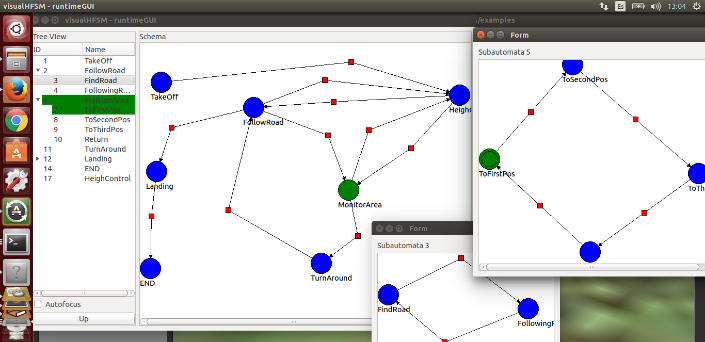
\includegraphics[height=5cm]{imgs/4_visualHFSM5/runtime-hierarchy.png}
	\caption{Multiples subautómatas en ejecución.}
	\label{fig:multipleSubautomatasGUI}
\end{figure}


%%%%%%%%%% Difusión %%%%%%%%%%%
\section{Difusión}
Una vez que hemos alcanzado una versión lo suficientemente madura de VisualHFSM 5.0, nos hemos centrado en darla a conocer para cumplir nuestro cuarto objetivo principal: convertirla en una herramienta utilizada por terceros. \\

Para conseguir esto, empezamos por elaborar una documentación sólida y detallada que explica cómo funciona VisualHFSM y las ventajas que ofrece, que puede encontrarse dentro de la página de JdeRobot\footnote{\url{http://jderobot.org/VisualHFSM}}. Esta documentación incluye:

\begin{itemize}
\item La entrada oficial de la herramienta dentro del manual de JdeRobot\footnote{\url{http://jderobot.org/Tools\#VisualHFSM}}, con una descripción básica, una explicación de su estructura y los detalles de cómo instalarla.
\item Un aviso de que la GUI en tiempo de ejecución está desactivada por defecto y una explicación de cómo ejecutar VisualHFSM si queremos ver esta GUI.
\item Una explicación detallada de cómo utilizar toda la funcionalidad que ofrece la herramienta, separando el editor gráfico, los componentes generados en C++ y los componentes generados en Python.
\item Un vídeo de ejemplo de un componente generado por la herramienta en ejecución, con un enlace a \textit{Running JdeRobot}\footnote{\url{http://jderobot.org/Running_JdeRobot\#VisualHFSM}}, dónde se explica detalladamente cómo ejecutar el ejemplo para poder probarlo.
\end{itemize}

Además, con el fin de dar a conocer VisualHFSM a la comunidad robótica, hemos escrito un artículo\cite{rey2016visualhfsm} al congreso robótico WAF\footnote{\url{http://waf2016.uma.es/}} (\textit{Workshop de Agentes Físicos}), explicando todas las novedades y ventajas que ofrece VisualHFSM 5.0. Este artículo ha sido aceptado y publicado en la edición del WAF de este año. Esto demuestra que la herramienta se centra en un tema que interesa a la comunidad robótica, y contamos con que llame la atención de futuros usuarios. \\

Por último, hemos introducido una práctica preparada para resolverla con VisualHFSM dentro del entorno docente de JdeRobot, \textit{Teaching Robotics}\footnote{\url{http://jderobot.org/Teaching_robotics_with_JdeRobot}}, que cuenta con una serie de prácticas distintas que se utilizan con fines didácticos en los cursos de JdeRobot y en las clases de róbotica de la Universidad Rey Juan Carlos. Al introducir una práctica basada en VisualHFSM damos la oportunidad a los alumnos de robótica de la universidad de futuros cursos a que utilicen la herramienta y aprendan a programar la inteligencia del robot en términos de estados y transiciones de una forma sencilla e intuitiva.

\vspace{1.5cm}
En este capítulo hemos descrito las distintas mejoras que aporta VisualHFSM 5.0 frente a las versiones anteriores y cómo éstas han sido implementadas. En el siguiente capítulo, expondremos varios casos de uso que validan estas mejoras.
\chapter{Resultados Experimentales}\label{chap:Experimentos}
En este capítulo presentaremos los experimentos más relevantes que hemos realizado utilizando la última versión de VisualHFSM. Aunque esta herramienta ya ha sido validada en versiones anteriores, con estos ejemplos buscamos validar el correcto funcionamiento de todas las mejoras introducidas, centrándonos especialmente en la nueva posibilidad de generar componentes en Python y en la GUI en ejecución. \\

Con estos experimentos, buscamos también demostrar que VisualHFSM es una herramienta útil y cómoda para programar el comportamiento de autómatas de una manera más rápida y sencilla. Además, nos sirven para demostrar el correcto funcionamiento de los componentes generados en Python, dado que los siguientes ejemplos usan esta funcionalidad, y probamos también que la herramienta es compatible con otro robot con el que no había sido probada hasta ahora: los drones.


%%%%%%%%%%%%%%% Ejemplo C++ %%%%%%%%%%%%%%%
\section{Cuadrado con un Pioneer}
La aplicación \textit{Cuadrado con un Pioneer}\footnote{\url{http://jderobot.org/S.rey-tfg\#TreeView_AutoFocus}} tiene como objetivo principal validar el correcto funcionamiento de las nuevas funcionalidades de VisualHFSM en los componentes generados en C++. Para esto hemos utilizado el robot \textit{Pioneer} simulado con Gazebo, y el diagrama de estados de la aplicación creado con el editor gráfico puede verse en la figura \ref{fig:squarePioneer}. \\

\begin{figure}[htbp]
	\centering
	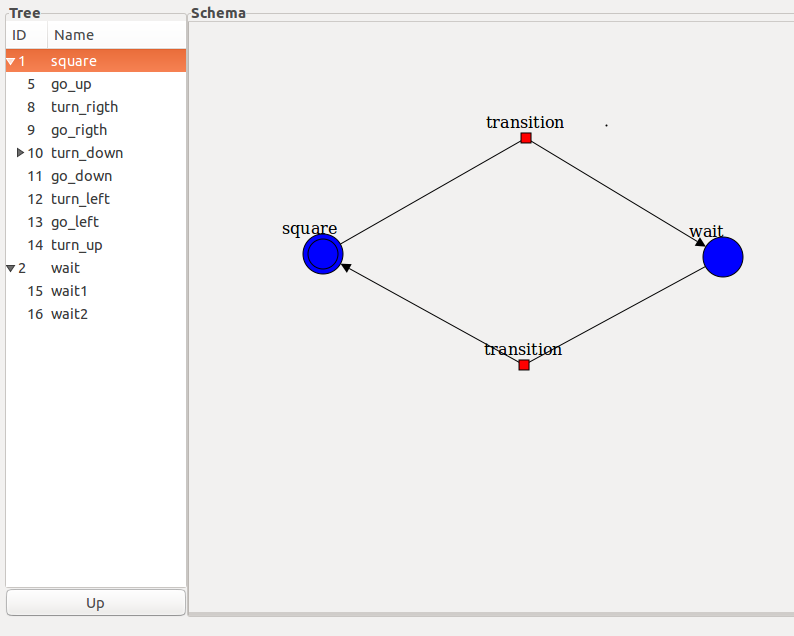
\includegraphics[height=7cm]{imgs/5_experiments/cuadradoPioneer.png}
	\caption{Aplicación Cuadrado con un Pioneer en el editor gráfico de VisualHFSM.}
	\label{fig:squarePioneer}
\end{figure}

En esta aplicación, con el fin de probar la robustez de los componentes generados en C++ en autómatas multinivel hemos desarrollado un comportamiento algo artificioso. El subautómata raíz consiste en dos estados: \textit{square} y \textit{wait}, con transiciones temporales entre ellos. La idea es que cuando esté en el estado \textit{square} se activará su subautómata hijo, y el robot empezará a moverse haciendo un cuadrado. Cuándo pase el tiempo definido en la transición temporal, el subautómata principal transitará al estado \textit{wait}, donde el robot se parará sin hacer nada hasta que vuelva a transitar. Este estado cuenta también con un subautómata hijo con dos estados, \textit{wait1} y \textit{wait2}, conectados por transiciones temporales. Nuevamente, en estos estados no se realiza ninguna acción. Adicionalmente, el estado \textit{turn\_down}, perteneciente al subautómata hijo del estado \textit{square}, también tiene un subautómata hijo con tres estados en los que tampoco se realiza ninguna acción. \\

El objetivo de todos estos estados vacíos es crear un autómata con varios niveles, para comprobar que la notificación de estados activos de la GUI en ejecución y la funcionalidad \textit{autofocus} funcionan correctamente en los componentes en C++. En las figuras \ref{fig:squarePioneerApp} y \ref{fig:waitPioneer} se pueden observar dos capturas de la ejecución de esta aplicación, observándose el correcto funcionamiento de la nueva funcionalidad.

%%%%IMAGENES EN FUNCIONAMIENTO

\begin{figure}[htbp]
	\begin{subfigure}{1\textwidth}
	\centering
	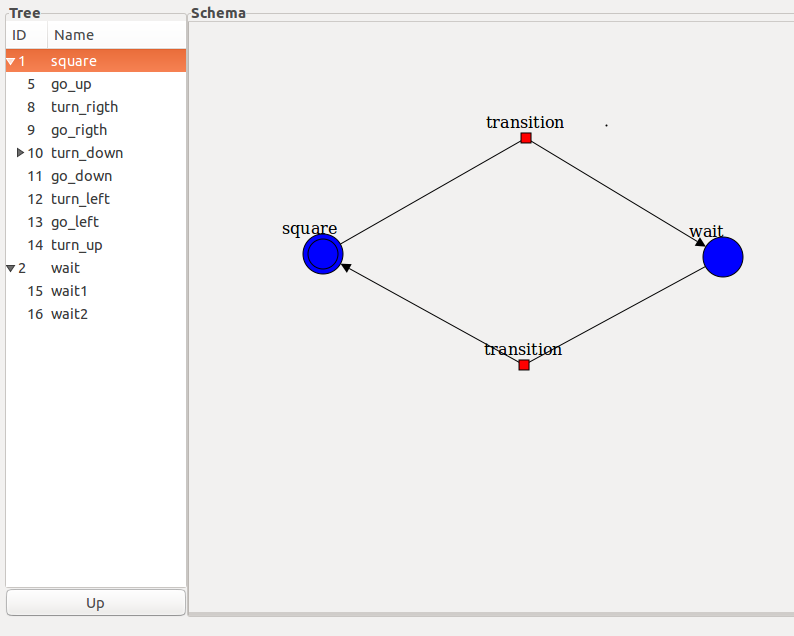
\includegraphics[height=6cm]{imgs/5_experiments/cuadradoPioneer.png}
	\caption{Estado \textit{square}.}
	\label{fig:squarePioneerApp}
	\end{subfigure}
	\hfill
	\begin{subfigure}{1\textwidth}
	\centering
	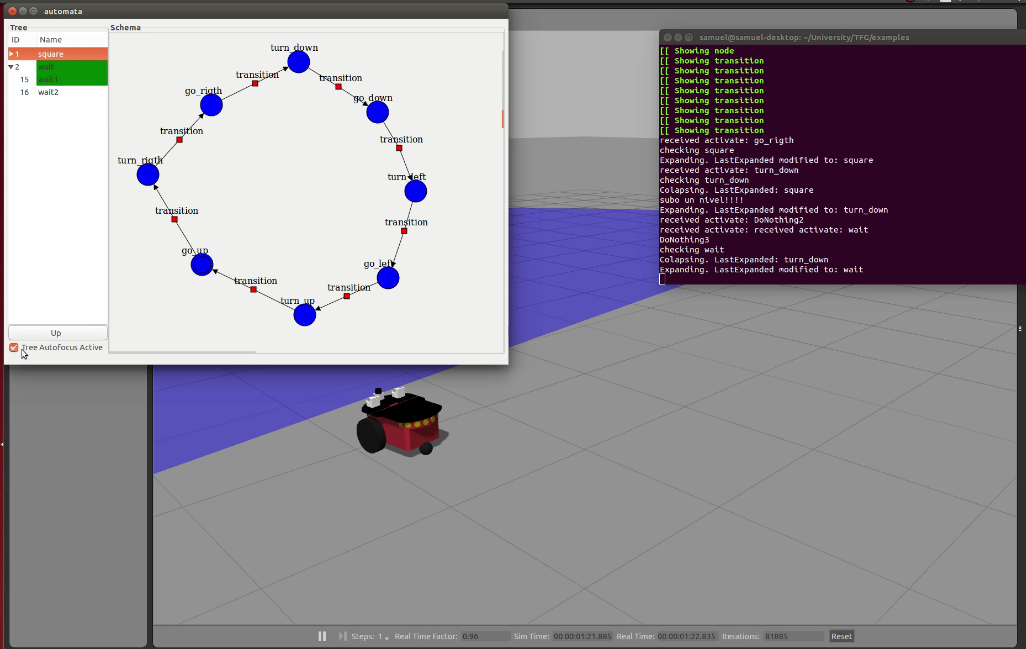
\includegraphics[height=5cm]{imgs/5_experiments/watingCuadradoPioneer.png}
	\caption{Estado \textit{wait}.}
	\label{fig:waitPioneer}
	\end{subfigure}
\caption{Aplicación Cuadrado con un Pioneer con GUI en tiempo de ejecución.}
\label{fig:squareApplication}
\end{figure}

%%%%%%%%%%%%%%% Bump & Go %%%%%%%%%%%%%%%
\section{Choca-Gira}
%%% Descripción
La primera aplicación en Python se llama \textit{Choca-Gira}\footnote{\url{http://jderobot.org/Teaching_robotics_with_JdeRobot\#Bump_and_go}}. Este sencillo ejemplo es la solución a la práctica dentro del entorno docente de JdeRobot que ya mencionamos en el capítulo anterior. El escenario inicial consta de un robot Kobuki situado en el centro de un laberinto. El robot debe avanzar recto hasta que detecte que se ha acercado demasiado a un obstáculo, en este caso una pared. Entonces, deberá retroceder un poco, girar un ángulo aleatorio, y volver a avanzar recto, repitiendo este proceso una y otra vez.  \\

\begin{figure}[htbp]
	\centering
	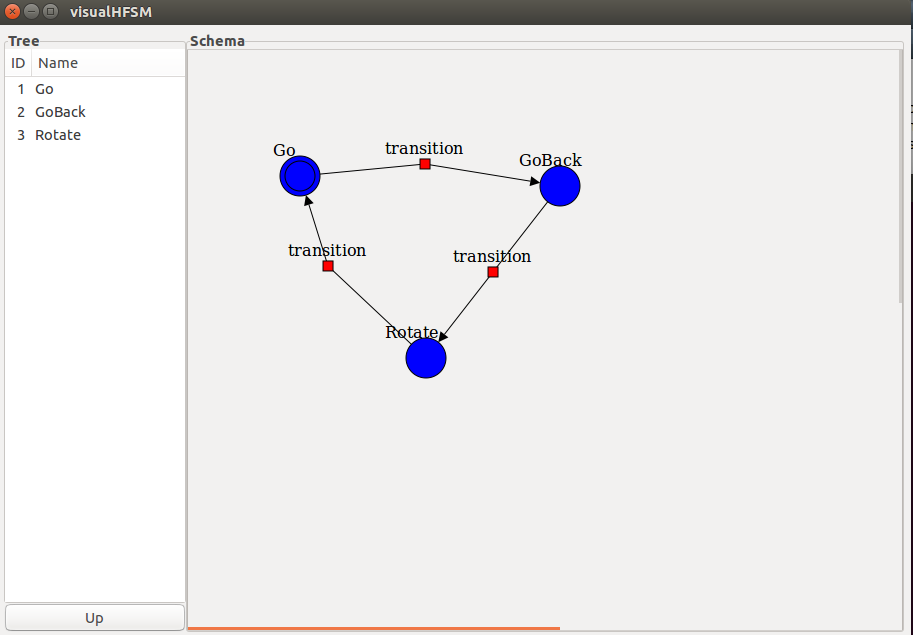
\includegraphics[height=7cm]{imgs/5_experiments/bumpAndGoDiagram.png}
	\caption{Aplicación Choca-Gira en el editor gráfico de VisualHFSM.}
	\label{fig:bumpAndGoDiagram}
\end{figure}

El diagrama de estados que representa este comportamiento puede verse en la figura \ref{fig:bumpAndGoDiagram}, donde se observa que cuenta con 3 estados: el estado inicial \textit{Go} (figura \ref{fig:BampAndGo-Go}), en el que únicamente va recto, pasando al estado \textit{GoBack} cuando se acerca demasiado a un obstáculo. Entonces retrocede por un tiempo determinado usando una transición temporal, y pasa al estado \textit{Rotate} (figura \ref{fig:BampAndGo-Rotate}), donde girará un ángulo aleatorio desde su posición. Una vez que ha alcanzado dicho ángulo, volverá al estado inicial. Una muestra de la ejecución de este experimento puede verse en la figura \ref{fig:bumpAndGo}, utilizando la GUI en tiempo de ejecución, observándose cómo se actualizan dinámicamente los estados activos en el \textit{Schema View} y en el \textit{Tree View} para este autómata mononivel. \\


%%% Motivación
El objetivo de este experimento era demostrar que con VisualHFSM es posible desarrollar comportamientos autónomos de robots introduciendo muy poco código. Además, hemos conseguido un ejemplo que puede servir de referencia a los alumnos que vayan a resolver este ejercicio en el entorno docente de JdeRobot en cursos futuros. \\

En la figura \ref{fig:statesCode} podemos observar el código en Python que hemos introducido utilizando el editor para que el comportamiento funcione correctamente. Con estas pocas líneas de código VisualHFSM es capaz de autogenerar el resto del código, incluido el introducido con la interfaz gráfica, consiguiendo la aplicación que hemos descrito. Adicionalmente, en el fragmento de código \ref{lst:bumpAndGoCode} podemos observar el código que ha generado nuestra herramienta a partir del código introducido en el editor para crear el único subautómata de esta aplicación.

\begin{lstlisting}[style=python,caption={Único subautómata de la aplicación Bump \& Go.},label={lst:bumpAndGoCode}]
def subautomata1(self):
		self.run1 = True
		cycle = 100
		t_activated = False
		t_fin = 0

		laserData = self.LasersPrx.getLaserData()
		minDistance = 1.5
		dist = None
		destinyAngle = None
		error = 0
		
		print "numero de lasers (grados):", laserData.numLaser
		

		while(self.run1):
			totala = time.time() * 1000000

			# Evaluation if
			if(self.sub1 == "Go"):
				if(dist != None and dist < minDistance):
					self.sub1 = "GoBack"
					self.MotorsPrx.setV(0)
					print "stopping"
					if self.displayGui:
						self.automataGui.notifySetNodeAsActive('GoBack')

			elif(self.sub1 == "GoBack"):
				if(not t_activated):
					t_ini = time.time()
					t_activated = True
				else:
					t_fin = time.time()
					secs = t_fin - t_ini
					if(secs > 1.5):
						self.sub1 = "Rotate"
						t_activated = False
						angle = self.getRobotTheta()
						print "my Angle:", angle
						self.MotorsPrx.setV(0)
						if self.displayGui:
							self.automataGui.notifySetNodeAsActive('Rotate')

			elif(self.sub1 == "Rotate"):
				if(error <= 0.1 and error >= -0.1):
					self.sub1 = "Go"
					destinyAngle =None
					self.MotorsPrx.setW(0)
					if self.displayGui:
						self.automataGui.notifySetNodeAsActive('Go')


			# Actuation if
			if(self.sub1 == "Go"):
				self.MotorsPrx.setV(1)
				laserData = self.LasersPrx.getLaserData()
				
				dist = None
				for i in range(60, 120):
					dist = laserData.distanceData[i]/1000
					if dist == None or laserData.distanceData[i]/1000 < dist:
						dist = laserData.distanceData[i]/1000
				
				print "dist:", dist
			elif(self.sub1 == "GoBack"):
				self.MotorsPrx.setV(-1)
				print "back"
			elif(self.sub1 == "Rotate"):
				if destinyAngle == None:
					turn = random.uniform(-math.pi, math.pi)
					destinyAngle = (angle + turn) % (math.pi)
					print "DestinyAngle:", destinyAngle
				
				angle =  self.getRobotTheta()
				error = (destinyAngle - angle)*0.75
				
				if error > 0 and error < 0.1:
					error = 0.1
				elif error < 0 and error > -0.1:
					error = -0.1
				
				print "angle:", angle, "destiny:", destinyAngle, "speed:", error
				self.MotorsPrx.setW(error)

			totalb = time.time() * 1000000
			msecs = (totalb - totala) / 1000;
			if(msecs < 0 or msecs > cycle):
				msecs = cycle
			else:
				msecs = cycle - msecs

			time.sleep(msecs / 1000)
			if(msecs < 33 ):
				time.sleep(33 / 1000);
\end{lstlisting}

\begin{figure}[htbp]
	\begin{subfigure}{1\textwidth}
	\centering
	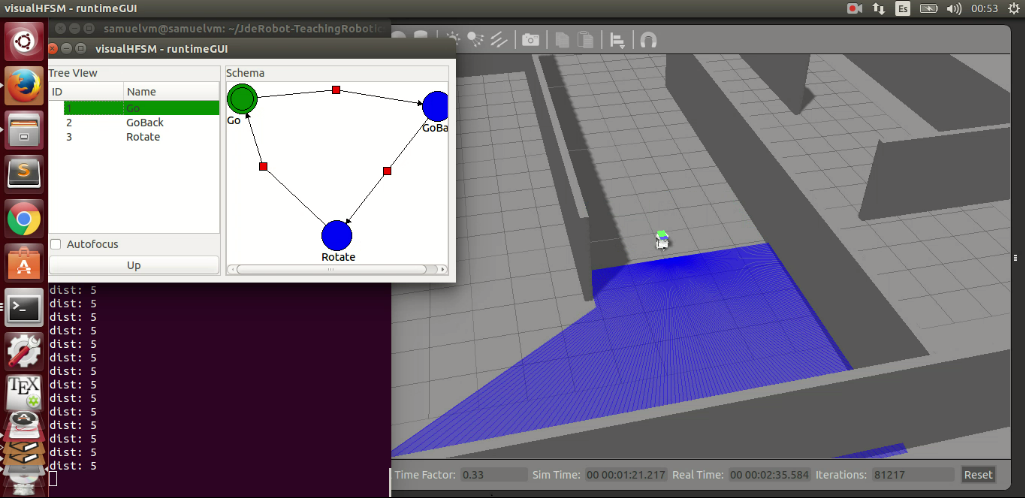
\includegraphics[height=5cm]{imgs/5_experiments/BAGFront.png}
	\caption{Estado Go.}
	\label{fig:BampAndGo-Go}
	\end{subfigure}
	\hfill
	\begin{subfigure}{1\textwidth}
	\centering
	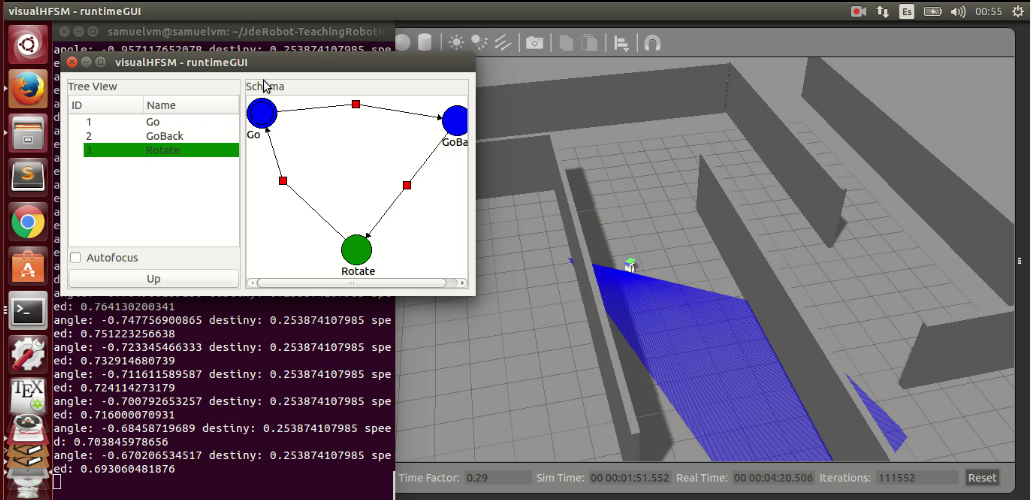
\includegraphics[height=5cm]{imgs/5_experiments/BAGRotate.png}
	\caption{Estado Rotate.}
	\label{fig:BampAndGo-Rotate}
	\end{subfigure}
\caption{Aplicación Choca-Gira con GUI en tiempo de ejecución.}
\label{fig:bumpAndGo}
\end{figure}

\begin{figure}[htbp]
	\begin{subfigure}{0.4\textwidth}
	\centering
	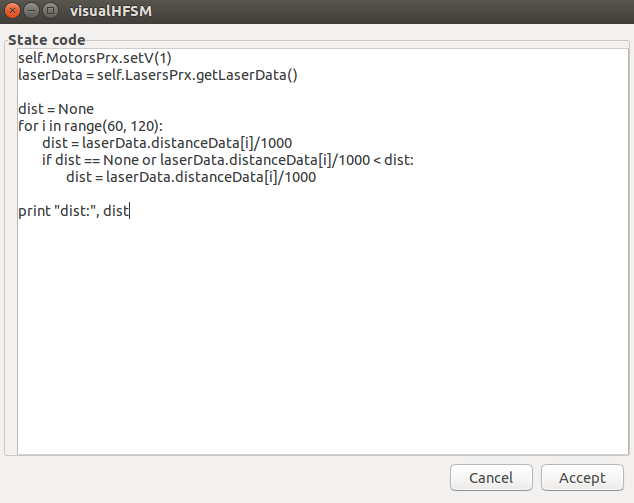
\includegraphics[height=6cm]{imgs/5_experiments/stateGo.png}
	\caption{Código del estado Go.}
	\label{fig:stateGo}
	\end{subfigure}
	\hfill
	\begin{subfigure}{0.4\textwidth}
	\centering
	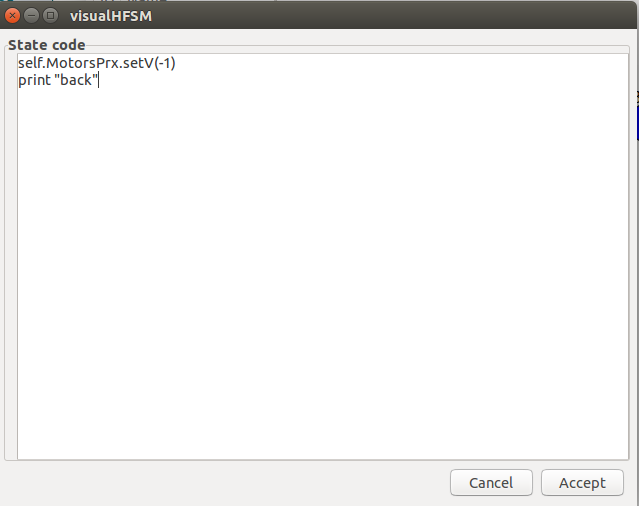
\includegraphics[height=6cm]{imgs/5_experiments/stateGoBack.png}
	\caption{Código del estado GoBack.}
	\label{fig:stateGoBack}
	\end{subfigure}
	\begin{subfigure}{1\textwidth}
	\centering
	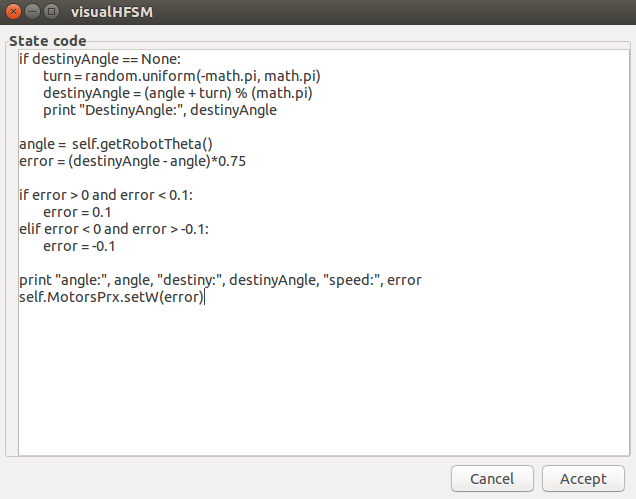
\includegraphics[height=6cm]{imgs/5_experiments/stateRotate.png}
	\caption{Código del estado Rotate.}
	\label{fig:stateRotate}
	\end{subfigure}
\caption{Código de los estados de la aplicación Bump \& Go.}
\label{fig:statesCode}
\end{figure}


%%%%%%%%%%%%%%% Monitor An Area %%%%%%%%%%%%%%%
\section{Monitorizar un área con un drone}
La aplicación \textit{Monitor an Area}\footnote{\url{http://jderobot.org/S.rey-tfg\#Monitor_Area_example}} simula un comportamiento más complejo que el anterior, representando un uso real en el que los drones podrían ser de utilidad. El mundo de este ejemplo simula un accidente de coche, con unas víctimas en el suelo, y para evaluarlas rápidamente se ha decidido enviar un drone autónomo para revisar con su cámara en qué estado se encuentran y poder acudir en su ayuda lo mejor preparados posibles. Para esto, el drone debe seguir la carretera hasta el punto en el que ha tenido lugar el accidente, encontrar a las víctimas, coger imágenes para que se evalúe su estado, y regresar.

\begin{figure}[htbp]
	\centering
	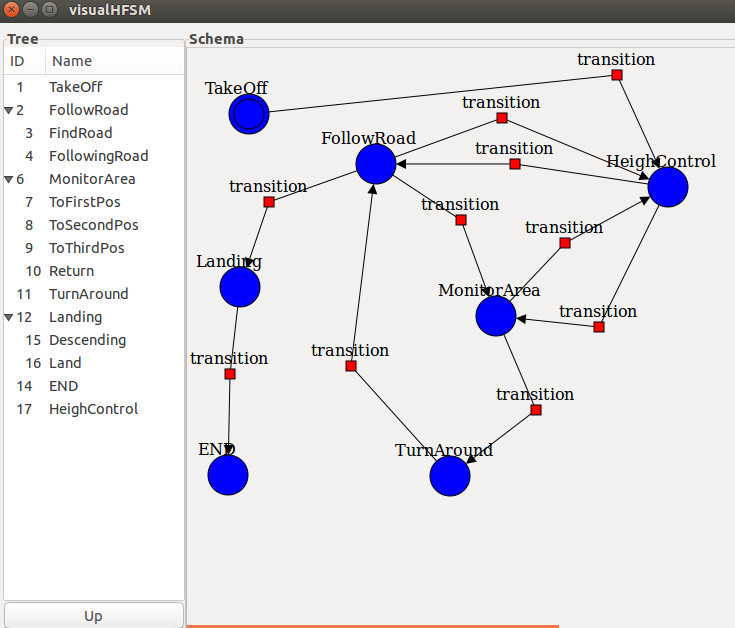
\includegraphics[height=7cm]{imgs/5_experiments/monitorArea.png}
	\caption{Aplicación Monitor an Area en el editor gráfico de VisualHFSM.}
	\label{fig:monitorDiagram}
\end{figure}

Estas distintas acciones que debe integrar el robot de forma autónoma pueden representarse perfectamente mediante un autómata de estados y transiciones, como el que muestra la figura \ref{fig:monitorDiagram}. Este esquema representa el comportamiento de un autómata jerárquico, en el que el comportamiento del robot es el siguiente:

\begin{enumerate}
\item Empieza despegando en el estado \textit{TakeOff}.
\item A continuación, pasa al estado \textit{HeightControl}, donde se alcanzará la altura deseada para seguir bien la carretera. A este estado se podrá transitar desde los demás estados otra vez en caso de que la altura se desvíe demasiado de la deseada, con la idea de corregir posibles derivas de alturas provocadas, por ejemplo, por corrientes de aire.
\item Tras alcanzar esta altura se transita al estado \textit{FollowRoad}, encargado de seguir la carretera. Este estado tiene un subautómata hijo con otros dos estados: \textit{FindRoad}, que será el estado encargado de encontrar la carretera otra vez si se perdiese de vista, y el estado \textit{FollowingRoad}, encargado de seguir la carretera una vez ha sido localizada. El hecho de dividir la tarea de seguir la carretera en estos dos estados facilita que el algoritmo empleado para encontrar otra vez la carretera pueda complicarse cuánto se desee sin necesidad de que esto afecte al seguimiento.
\item Cuando el drone ha llegado al punto en el que el accidente tuvo lugar (en este caso por simplicidad hemos supuesto que se sabía las coordenadas), se pasa al estado \textit{MonitorArea}. Este estado es el encargado de buscar a las víctimas. En esta ocasión, nuevamente por simplificar el código del ejemplo, hemos supuesto que se sabía el número de víctimas y su ubicación GPS exacta, por lo que el estado cuenta con un subautómata con un estado para acudir a la posición de cada víctima mediante un sistema de control PID, y un último estado para regresar a la posición en la que abandonó la carretera.
\item Cuando regresa a la carretera transita al estado \textit{TurnAround}, que hará que el drone rote 180 grados para poder seguir la carretera en sentido contrario.
\item Cuando ha terminado de dar la vuelta, regresa al estado \textit{FollowRoad}, siguiendo nuevamente la carretera hasta llegar al punto donde despegó.
\item Una vez que el drone está sobre la posición de la que salió en un primer momento, se activará el estado \textit{Landing}. Nuevamente, este estado tiene un subautómata hijo para conseguir que el aterrizaje sea suave. Primero se activará el estado \textit{Descending}, que se encargará de que el drone pierda altura antes de que se de la orden de aterrizar, de forma que cuando la altura es la deseada, el estado activo pasará a ser \textit{Land}, donde el drone terminará el aterrizaje.
\item Por último, el estado \textit{END} simplemente llamará a la función \emph{shutDown()} para que se termine la ejecución de la aplicación.
\end{enumerate}

\begin{figure}[htbp]
	\begin{subfigure}{1\textwidth}
	\centering
	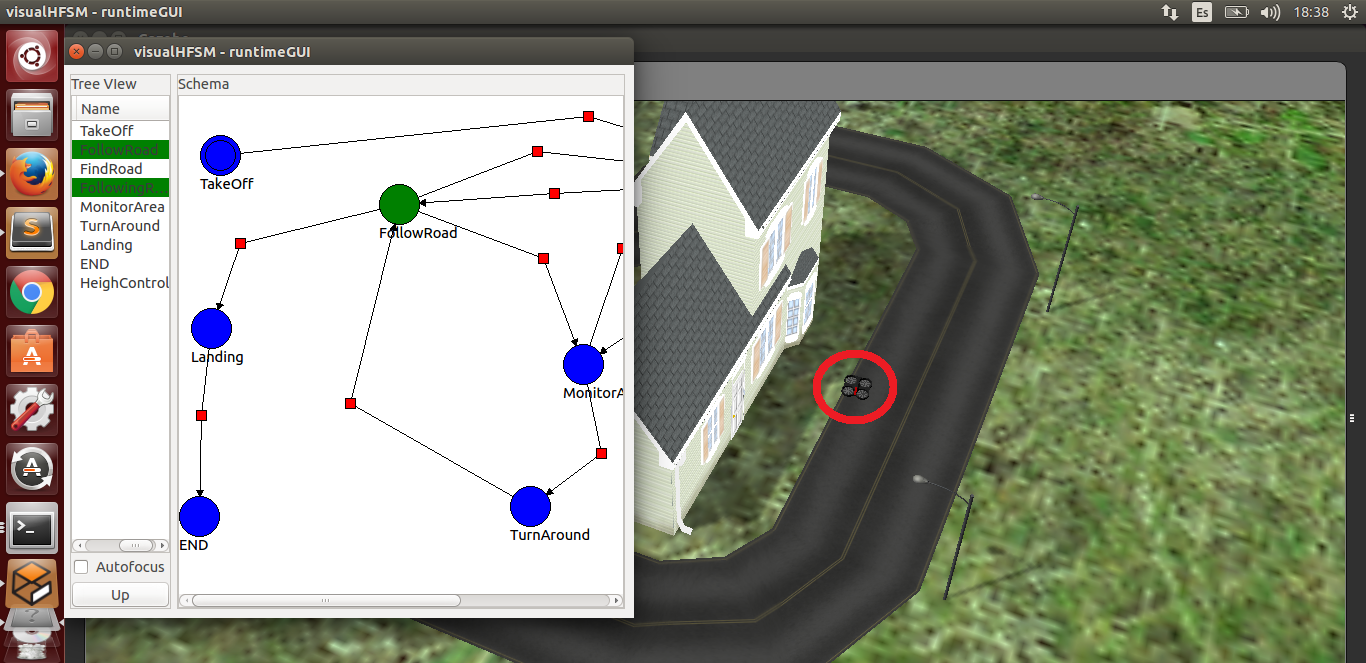
\includegraphics[height=4.5cm]{imgs/5_experiments/followingRoad.png}
	\caption{Siguiendo la carretera.}
	\label{fig:followingRoad}
	\end{subfigure}
	\hfill
	\begin{subfigure}{1\textwidth}
	\centering
	\includegraphics[height=4.5cm]{imgs/5_experiments/watchPerson.png}
	\caption{Monitorizando a una de las víctimas.}
	\label{fig:watchPerson.png}
	\end{subfigure}
\caption{Aplicación Monitor an Area con GUI en ejecución.}
\label{monitorArea}
\end{figure}

Si observamos la figura \ref{monitorArea} podemos ver imágenes de la aplicación en ejecución en distintos estados, utilizando la GUI en tiempo de ejecución para representar dinámicamente que estados se encuentran activos. En la figura \ref{fig:followingRoad} se puede observar al ArDrone siguiendo la carretera, y la figura \ref{fig:watchPerson.png} muestra cómo el ArDrone ha llegado hasta una se sus víctimas. Además, si nos fijamos en el fragmento de código \ref{lst:createAutomataMonitorArea}, podemos ver la función \texttt{createAutomata()}, que es la responsable de crear la lista de subautómatas que permite generar la GUI en ejecución sin depender del archivo XML. \\

Con este ejemplo también probamos los interfaces del ArDrone, que ahora está soportado en VisualHFSM. Además se prueba la robustez de los componentes generados por nuestra herramienta utilizando un diagrama de estados de mayor complejidad y con distintos niveles de jerarquía, y, por tanto varios subautómatas con sus respectivos hilos corriendo simultáneamente. Sirve también para probar la robustez de la GUI en ejecución, su navegación, y especialmente el correcto funcionamiento de la funcionalidad \textit{autofocus} que ofrece, que sólo tiene sentido en autómatas multinivel. \\ \\


\begin{lstlisting}[style=python,caption={Función \texttt{createAutomata()} de la aplicación Monitor an Area.},label={lst:createAutomataMonitorArea}]

	def createAutomata(self):
		guiSubautomataList = []

		# Creating subAutomata1
		guiSubautomata1 = GuiSubautomata(1,0, self.automataGui)

		guiSubautomata1.newGuiNode(1, 0, 62, 66, 1, 'TakeOff')
		guiSubautomata1.newGuiNode(2, 3, 189, 116, 0, 'FollowRoad')
		guiSubautomata1.newGuiNode(6, 5, 309, 268, 0, 'MonitorArea')
		guiSubautomata1.newGuiNode(11, 0, 263, 428, 0, 'TurnAround')
		guiSubautomata1.newGuiNode(12, 6, 53, 239, 0, 'Landing')
		guiSubautomata1.newGuiNode(14, 0, 41, 427, 0, 'END')
		guiSubautomata1.newGuiNode(17, 0, 481, 139, 0, 'HeighControl')

		guiSubautomata1.newGuiTransition((189, 116), (309, 268), 
										(274, 172), 7, 2, 6)
		guiSubautomata1.newGuiTransition((309, 268), (263, 428), 
										 (349, 362), 13, 6, 11)
		guiSubautomata1.newGuiTransition((263, 428), (189, 116), 
										 (164, 318), 14, 11, 2)
		guiSubautomata1.newGuiTransition((189, 116), (53, 239), 
										 (82, 154), 19, 2, 12)
		guiSubautomata1.newGuiTransition((53, 239), (41, 427), 
										 (43, 326), 22, 12, 14)
		guiSubautomata1.newGuiTransition((481, 139), (189, 116), 
										 (328, 116), 26, 17, 2)
		guiSubautomata1.newGuiTransition((62, 66), (481, 139), 
										 (430, 27), 27, 1, 17)
		guiSubautomata1.newGuiTransition((189, 116), (481, 139), 
										 (315, 70), 28, 2, 17)
		guiSubautomata1.newGuiTransition((309, 268), (481, 139), 
										 (378, 195), 29, 6, 17)
		guiSubautomata1.newGuiTransition((481, 139), (309, 268), 
										 (412, 279), 30, 17, 6)
		guiSubautomataList.append(guiSubautomata1)

		# Creating subAutomata3
		guiSubautomata3 = GuiSubautomata(3,2, self.automataGui)

		guiSubautomata3.newGuiNode(3, 0, 156, 228, 1, 'FindRoad')
		guiSubautomata3.newGuiNode(4, 0, 427, 255, 0, 'FollowingRoad')

		guiSubautomata3.newGuiTransition((156, 228), (427, 255), 
										 (297, 157), 2, 3, 4)
		guiSubautomata3.newGuiTransition((427, 255), (156, 228), 
										 (265, 320), 3, 4, 3)
		guiSubautomataList.append(guiSubautomata3)

		# Creating subAutomata5
		guiSubautomata5 = GuiSubautomata(5,6, self.automataGui)

		guiSubautomata5.newGuiNode(7, 0, 86, 275, 1, 'ToFirstPos')
		guiSubautomata5.newGuiNode(8, 0, 247, 92, 0, 'ToSecondPos')
		guiSubautomata5.newGuiNode(9, 0, 491, 303, 0, 'ToThirdPos')
		guiSubautomata5.newGuiNode(10, 0, 281, 455, 0, 'Return')

		guiSubautomata5.newGuiTransition((86, 275), (247, 92), 
										 (166, 184), 9, 7, 8)
		guiSubautomata5.newGuiTransition((247, 92), (491, 303), 
										 (369, 198), 10, 8, 9)
		guiSubautomata5.newGuiTransition((491, 303), (281, 455), 
										 (386, 379), 11, 9, 10)
		guiSubautomata5.newGuiTransition((281, 455), (86, 275), 
										 (184, 365), 12, 10, 7)
		guiSubautomataList.append(guiSubautomata5)

		# Creating subAutomata6
		guiSubautomata6 = GuiSubautomata(6,12, self.automataGui)
		guiSubautomata6.newGuiNode(15, 0, 126, 185, 1, 'Descending')
		guiSubautomata6.newGuiNode(16, 0, 350, 190, 0, 'Land')

		guiSubautomata6.newGuiTransition((126, 185), (350, 190), 
										 (232, 220), 24, 15, 16)
		guiSubautomataList.append(guiSubautomata6)

		return guiSubautomataList

\end{lstlisting}


%%%%%%%%%%%%%%% Sigue Colores %%%%%%%%%%%%%%%
\section{Aplicación Sigue Colores con un drone}
Esta aplicación también utiliza un drone, y aunque el comportamiento es más artificioso que la anterior, está orientada a ser ejecutada en robots reales, mostrando que los componentes generados mediante VisualHFSM se conectan también a drones reales, no sólo en los simulados. El ejercicio consiste en un drone, que tendrá que ser capaz de buscar y seguir objetos de distintos colores que detecte mediante filtros de color por su cámara ventral en un orden determinado. La secuencia es: seguir al verde hasta encontrar un color azul, entonces seguir al azul hasta encontrar otro verde. En este caso se volverá a seguir al verde hasta que detecte un color rojo, pasando entonces a seguir a este color hasta que el usuario decida terminar la ejecución. Es importante que el drone sea capaz de ignorar todos los colores que no estén relacionados con el estado actual. Esto es, si estando en el estado \textit{FollowGreenLookBlue} pasase bajo su cámara algo de color rojo, el drone debería ignorarlo. Esto muestra la mayor potencia del autómata frente a sistemas reactivos puros.

\begin{figure}[htbp]
	\centering
	\includegraphics[height=7cm]{imgs/5_experiments/colorsDiagram.png}
	\caption{Aplicación Sigue Colores en el editor gráfico de VisualHFSM.}
	\label{fig:colorsDiagram}
\end{figure}

En la figura \ref{fig:colorsDiagram} puede observarse el diagrama de estados que se encarga de resolver esta situación. Se parte de un estado \textit{TakeOff}, en el que el drone se elevará hasta alcanzar una altura determinada. Cuando esta altura ha sido alcanzada, transitará al estado \textit{FollowGreenLookBlue}. Este estado se encarga de coger las imágenes de la camára ventral y filtrarlas buscando color verde para seguirlo, y color azul, para pasar al siguiente estado en caso de encontrarlo. Cuenta además con un subautómata hijo que se encarga de seguir el color verde que su padre ha localizado. Para esto, el subautómata empieza en el estado \textit{WaitGreen}, en el cual esperará sin hacer nada hasta que su padre detecte el color verde, en cuyo caso se activará el estado \textit{FollowGreen}, que se encargará de seguirlo utilizando un PID. En este caso hemos optado por quedarnos parados hasta encontrar un color verde porque buscábamos un algoritmo que no fuese demasiado complejo para probarlo con robots reales. Además, el experimento está pensado para realizarse en un laboratorio, un espacio cerrado y por lo tanto limitado. Esta forma de seguir al color se ha implementado igual en todos los estados, por lo que todos cuentan con un subautómata hijo. \\

Una vez que se detecta un color azul, el subautómata raíz transitará al estado \textit{FollowBlueLookGreen}, donde seguirá al nuevo color azul hasta que encuentre un color verde. En este caso, para evitar que detecte automáticamente el color verde del estado anterior, se ha dejado un periodo refractario en el que el estado sólo buscará el color azul, y pasado este periodo empezará a buscar también el color verde, de forma que cuando lo encuentre, pasará al estado \textit{FollowGreenLookRed}. Este estado funciona igual que el primer estado que seguía el color verde, pero en lugar de buscar el color azul para transitar, ahora buscará el color rojo. Por último, cuando se detecte el color rojo, se pasará al estado \textit{FollowRed}, dónde únicamente buscará y seguirá el color rojo hasta que el usuario decida interrumpir la ejecución. \\

\begin{figure}[htbp]
	\centering
	\includegraphics[height=8cm]{imgs/5_experiments/functionsColors.png}
	\caption{Funciones comunes declaradas usando el editor gráfico.}
	\label{fig:functionsColors}
\end{figure}

También hemos utilizado la funcionalidad de crear variables y funciones comunes a todo el autómata, ofrecida por VisualHFSM, para evitar repetir código y que el resultado sea un componente más limpio. De esta forma, tal y como se observa en la figura \ref{fig:functionsColors}, hemos creado varias funciones necesarias en todos los estados encargados de buscar colores, de forma que el código queda más limpio y legible. Esto puede observarse en el fragmento de código \ref{lst:actuationIfFollowColors}, que muestra el \textit{if} de actuación del subautómata raíz de esta aplicación.

\begin{lstlisting}[style=python,caption={\textit{Actuation if} del subautómata raíz de la aplicación Sigue Colores.},label={lst:actuationIfFollowColors}]
	# Actuation if
	if(self.sub1 == "TakeOff"):
		if self.hIters == 0:
			self.ExtraPrx.takeoff()
			print "taking off"
		else:
			self.setVelocity(0,0,1,0)
		
		self.hIters += 1
		print "ITERS: ", self.hIters
	elif(self.sub1 == "FollowGreenLookBlue"):
		inImg = self.getImage()
		softenedImg = cv2.bilateralFilter(inImg, 9, 75, 75)
		self.greenConts, hierarchy = self.getContours(softenedImg,
													 minGValues, maxGValues)
		self.blueConts,  hierarchy = self.getContours(softenedImg,
													  minBValues, maxBValues) 
				
						
	elif(self.sub1 == "FollowBlueLookGreen"):
		inImg = self.getImage()
		softenedImg = cv2.bilateralFilter(inImg, 9, 75, 75)
		self.blueConts,  hierarchy = self.getContours(softenedImg,
													  minBValues, maxBValues) 
				
		if refracIters >= refracTime:
			self.greenConts, hierarchy = self.getContours(softenedImg,
													  minGValues, maxGValues)
			print "inside refrac time"
		else:
			print "refrac Iters:", refracIters
				
		refracIters += 1
	elif(self.sub1 == "FollowGreenLookRed"):
		inImg = self.getImage()
		softenedImg = cv2.bilateralFilter(inImg, 9, 75, 75)
		self.greenConts, hierarchy = self.getContours(softenedImg,
													  minGValues, maxGValues)
		self.redConts,  hierarchy = self.getContours(softenedImg,
													  minRValues, maxRValues)
		print "RED:", self.redConts
	elif(self.sub1 == "FollowRed"):
		inImg = self.getImage()
		softenedImg = cv2.bilateralFilter(inImg, 9, 75, 75)
		self.redConts, hierarchy = self.getContours(softenedImg,
													  minRValues, maxRValues)
\end{lstlisting}

Aunque el experimento está pensado para ejecutarse en robots reales, para depurar y validar el código hemos utilizado antes un simulador. Para esto, hemos utilizado el ArDrone, y 3 robots con ruedas de color verde, azul y rojo, que pueden ser teleoperados utilizando la herramienta \textit{kobukiViewer} de JdeRobot para comprobar que efectivamente el drone les está siguiendo. Esto puede verse en la figura \ref{fig:colorsSim}, donde se observa el drone simulado siguiendo al robot verde (figura \ref{fig:followingGreenSim}) y al rojo (\ref{fig:followingRoad}).

\begin{figure}[htbp]
	\begin{subfigure}{1\textwidth}
	\centering
	\includegraphics[height=6cm]{imgs/5_experiments/followingGreenSim.png}
	\caption{Siguiendo el Pioneer verde simulado.}
	\label{fig:followingGreenSim}
	\end{subfigure}
	\hfill
	\begin{subfigure}{1\textwidth}
	\centering
	\includegraphics[height=6cm]{imgs/5_experiments/followingRedSim.png}
	\caption{Siguiendo el Pioneer rojo simulado.}
	\label{fig:followingRedSim}
	\end{subfigure}
\caption{Aplicación Sigue Colores en Gazebo.}
\label{fig:colorsSim}
\end{figure}

Una vez que hemos validado el correcto funcionamiento del componente generado en el simulador, nos hemos preparado para probarlo en el mundo real. Para esto, hemos sustituido los robots de tres ruedas por cartulinas de colores que nosotros movemos para que el drone las siguiese, pero nos hemos encontrado con algunas dificultades. En primer lugar, el robot real no ofrece información real sobre su altura, por lo que hemos medido la altura deseada por el número de iteraciones que pasaban hasta que la alcanzase. Esto ya lo sabíamos en la versión simulada pero era necesario comprobar que la altura era la correcta fuera de Gazebo. \\

Los dos grandes retos a los que nos hemos enfrentado en el mundo real han sido: los filtros de color y la poca estabilidad del robot real. La principal diferencia entre el mundo real y el simulado es la luz, que en las simulaciones es mucho más uniforme. Sin embargo, en la realidad hay muchos brillos y puede variar mucho de un momento a otro, o de una zona a otra, incluso dentro de la misma aula. Esto hace que realizar un buen filtro de color robusto sea muy complicado. Adicionalmente, en el simulador el robot real es completamente estable, pero no en la realidad. De hecho, tiene una pequeña deriva hacia un lado, lo que provocaba que cuando debería quedarse quieto esperando encontrar un color, en verdad se movía constantemente a un lado ocasionando que se chocase. \\

En la figura \ref{fig:colorsReal} podemos observar la ejecución de esta aplicación utilizando un drone real, observándola siguiendo la cartulina verde en la imagen \ref{fig:followingGreen}, y la roja en la figura \ref{fig:followingRed}.

\begin{figure}[htbp]
	\begin{subfigure}{1\textwidth}
	\centering
	\includegraphics[height=5cm]{imgs/5_experiments/followingGreen.jpg}
	\caption{Siguiendo la cartulina verde.}
	\label{fig:followingGreen}
	\end{subfigure}
	\hfill
	\begin{subfigure}{1\textwidth}
	\centering
	\includegraphics[height=5cm]{imgs/5_experiments/followingRed.jpg}
	\caption{Siguiendo la cartulina roja.}
	\label{fig:followingRed}
	\end{subfigure}
\caption{Aplicación Sigue Colores utilizando un drone real.}
\label{fig:colorsReal}
\end{figure}

%%%%%%%%%%%%%%% Sigue Colores %%%%%%%%%%%%%%%
%\section{COMPORTAMIENTO SUPER CHULO EN C++}
\chapter{Conclusiones}\label{chap:Conclusiones}
Para finalizar, en este capítulo evaluaremos las soluciones que se han desarrollado para alcanzar los objetivos propuestos, y comentaremos algunas posibles líneas de trabajos futuros.


\section{Conclusiones}
Este TFG pretendía conseguir una versión más madura de VisualHFSM con el fin de que pudiese ser utilizada por terceros. Con esto en mente, habíamos establecido cuatro objetivos principales:

\begin{enumerate}
\item Mejorar la usabilidad del editor gráfico de la herramienta.
\item Recuperar la GUI en tiempo de ejecución para los autómatas multinivel.
\item Añadir la posibilidad de crear componentes en Python, aumentando así la flexibilidad de la herramienta.
\item Fomentar la difusión de la herramienta para darla a conocer, facilitando así que pueda ser utilizada por terceros.
\end{enumerate}

La conclusión general es que estos objetivos se han cumplido satisfactoriamente. Se ha conseguido una versión más robusta de la herramienta que ofrece nuevas funcionalidades muy útiles, dotándola de mayor flexibilidad y más facilidad para depurar el código, demostrando su correcto funcionamiento mediante varios ejemplos de distintos tipos. Además, se ha hecho un gran esfuerzo para la difusión y se ha mejorado toda la documentación para que el primer contacto sea lo más natural y sencillo posible, dejando la práctica \textit{choca-gira} para que los alumnos de robótica de la URJC utilicen esta herramienta en los próximos cursos. \\

Como hemos basado todo el trabajo en una herramienta ya existente, el primer paso ha sido conocer todo el código y la funcionalidad que ofrecía la herramienta, para utilizarlo de base. Además, hemos intentado reaprovechar al máximo todo el código posible, evitando duplicarlo para hacer más fácil su mantenimiento. Un claro ejemplo de esto es que la GUI en tiempo de ejecución de los componentes generados es prácticamente igual a la GUI del editor gráfico. \\

Centrándonos en la mejora de la usabilidad de la herramienta y mejorar la experiencia de usuario, hemos introducido una nueva forma de navegar a través de los nuevos niveles de la jerarquía, permitiendo mostrar el nivel deseado haciendo click en cualquiera de los estados que pertenezcan a él dentro del \textit{Tree View}. También hemos resuelto los problemas de dependencias que existían en las versiones anteriores haciendo posible abrir la herramienta desde cualquier directorio, de forma que no es necesario tener una carpeta con el código fuente que utilizan las distintas GUIs y ejecutarlo desde ahí para que funcione. \\

Otra mejora del editor gráfico ha sido el aumento de flexibilidad en la creación de los archivos de configuración para ICE. Ahora permite elegir el nombre de la \textit{proxy} con el que se conectará a la interfaz ICE, permitiendo así que los componentes generados por VisualHFSM puedan conectarse a las \textit{proxys} de cualquier aplicación, haciendo posible que el código funcione cómodamente con robots reales. Además, se ha hecho de forma compatible con los proyectos obtenidos mediante versiones anteriores, dado que si no se ha determinado un nombre para la \textit{proxy}, entonces sí dependerá de la interfaz que se esté utilizando. \\

La primera mejora grande de la herramienta afecta a los componentes generados por VisualHFSM, recuperando la GUI en ejecución. Esta característica es realmente útil en los procesos de depuración y se perdió al hacer que VisualHFSM soportase autómatas multinivel. Fue la motivación inicial de este proyecto. Para que el aspecto de todas las GUI fuese lo más similar posible y otorgar una sensación de unidad a toda la herramienta, se adaptó el la GUI ya existente en el editor gráfico, eliminando funcionalidades y \textit{widgets} no necesarios, y añadiendo otros que sí eran útiles. \\

La segunda gran mejora de esta versión de VisualHFSM es que hemos añadido al generador de código la capacidad de crear componentes en Python. Esto le añade una mayor flexibilidad, aumentando el número de posibles usuarios que podrían utilizarla, dado que en el mundo de la robótica se está utilizando Python como lenguaje de programación de forma cada vez más común. Para hacer esto posible hemos modificado el generador de código, creando una nueva plantilla desde cero para los autómatas, siguiendo un modelo de programación orientada a objetos. Además, se ha buscado también que el aspecto sea lo más similar posible a la del editor y a la de los componentes generados en C++. Esta posibilidad de generar componentes en Python no reemplaza a los componentes en C++, sino que lo complementa, siendo compatibles los dos modelos. \\

En relación a la difusión de la herramienta para fomentar su uso, también hemos conseguido avances satisfactorios. Empezamos por escribir una documentación sólida en la web de JdeRobot, dado que la anterior trataba de versiones demasiado antiguas, por lo que no resultaba útil. En esta documentación se explican detalladamente todos los aspectos de la herramienta, así como una descripción y sus características generales, o los pasos que hay que realizar para instalar este componente, en caso de que quiera instalarse aparte del resto de componentes de JdeRobot. También se detalla toda la funcionalidad que ofrece y cómo utilizarla, así como de qué manera hay que ejecutarla, en función de si queremos o no utilizar la GUI en ejecución. Por último, esta documentación incluye también un vídeo que muestra un componente en ejecución generado con VisualHFSM 5.0, y una explicación detallada de los pasos que hay que seguir para ejecutarlo, permitiendo así probar con un ejemplo hecho que todo funciona correctamente, y poder tomarlo como primer paso para jugar con él probando las funcionalidades que ofrece la nueva herramienta. \\

Además de esta documentación, ha sido importante la difusión de la herramienta. Hemos escrito un artículo en el congreso científico WAF, publicado comentando todas las ventajas que ofrece VisualHFSM 5.0. Esto demuestra que VisualHFSM aborda un tema que realmente interesa en el mundo de la robótica y nos otorga una gran oportunidad para dar a conocer esta herramienta y sus ventajas, pudiendo ganar usuarios potenciales. \\

Por último, dentro de esta tarea de difusión, hemos introducido una práctica dentro del entorno docente de  JdeRobot  que utiliza como plataforma VisualHFSM. Esto permite a los alumnos que la realicen tener un primer acercamiento a los autómatas, y comprobar las facilidades que supone para el desarrollo de comportamientos de robots. \\

Para finalizar esta sección, comentar que todas las mejoras introducidas con esta versión que se han resumido en las conclusiones se traducen en un desarrollo software con más de 2500 líneas de código. Esto, sin contar el diseño de las GUIs en tiempo de ejecución, los mundos creados con Gazebo para la validación experimental, las aplicaciones creadas ni la documentación escrita. Estás son únicamente las líneas de código de la herramienta que se han añadido a las versiones ya existentes.


\section{Trabajos futuros}
Aunque VisualHFSM 5.0 es una versión mucho más madura y completa que las anteriores, aún presenta algunos aspectos que podrían mejorarse, teniéndose en cuenta para posibles líneas de trabajo futuras. \\

Aunque la GUI en tiempo de ejecución supone una gran ayuda para la depuración del código, aún se le podría añadir funcionalidad para que resulte incluso más útil. Por ejemplo, a veces es conveniente saber el valor de ciertas variables, además de ver en que estado se encuentra. Una posible mejora podría ser añadir a la GUI en tiempo de ejecución un nuevo espacio, el \textit{Data View}, utilizado para mostrar las variables y su valor que le interesen al desarrollador. Sería necesario un \textit{built-in} que el usuario pueda llamar desde el código del componente para indicar qué quiere mostrar o actualizar una variable y su valor. \\

Una limitación que hemos comprobado al probar los componentes con drones reales es que una vez que se empieza a ejecutar el componente generado, no hay forma de detener la ejecución, dado que si se interrumpe desde el terminal el robot no se detendrá, si no que seguirá en la última velocidad que el programa le haya mandado. Esto puede dar problemas, si el código no se comporta como el desarrollador espera puede hacer que el robot se choque. Por esto, sería útil incluir un \emph{botón de parada de emergencia}, para detener el robot e interrumpir la ejecución del componente. El problema que esto plantea es que la forma de establecer la velocidad a cero depende del tipo de robot, por lo que habría que hacer que sea el usuario quien cree esta función, que será llamada al pulsar el botón. \\

Por último, en esta memoria hemos comentado que una de las claras ventajas de los lenguajes de programación visual es que al ser tan naturales y legibles son especialmente útiles para la docencia. Por lo tanto, podría resultar de utilidad acercar VisualHFSM aún más a los lenguajes gráficos, dando la posibilidad de crear una serie de estados preprogramados como instrucciones gráficas. Por ejemplo, moverse, de forma que el usuario sólo tenga que introducir la velocidad con la que quiera que se mueva el robot, pudiendo conseguir así que niños programasen comportamientos sencillos de robots, acercándonos al estilo de Scratch o Blockly.

%%%%%%%%%%%%%%% Bibliografía %%%%%%%%%%%%%%%
\nocite{*}
\bibliographystyle{acm}
\bibliography{biblio}
\end{document}
